%!TEX root = ../my_thesis.tex
\section{Optimisation of the opposite-side electron tagger}
\label{sec:tagging:OSeOpt}

%%%%%%%%%%%%%%%%%%%%%%%%%%%%%%%%%%%%%%%%%%%%%%%%%%%%

The performance of the flavour tagging algorithms depends on the data taking conditions, in particular the centre-of-mass energy
of the $pp$ collision. 

On one hand, the tagging power of the SS taggers shows an increase on Run 2 data as compared to Run 1, thanks to either a higher tagging efficiency (\SSpi~and \SSp) or a lower mistag rate (\SSK). This is due to the higher boost of the $b\bar b$ quark pair at $13~\rm TeV$, which makes the momentum spectrum of $B$ mesons and fragmentation tracks harder, and increases the acceptance of the fragmentation tracks. 

On the other hand, the tagging power of the existing \OSe, \OSmu, and \OSK~taggers decreases on Run 2 data. The reason for this degradation is mainly due to the higher track multiplicity, which increases the probability to have a wrong tag decision. Moreover, because of the different Run 2 kinematics, the criteria to select the tagging particles are no longer optimal, thus giving a lower tagging efficiency.

The performance of the \OSc~and~\OSvtx~algorithms is, on average, compatible or better on Run 2 as compared to Run 1.

In this section, the reoptimisation of the \OSe~tagger is presented. This reoptimisation is performed both on Run 2 data, in order to recover the observed loss in tagging power, and on Run 1 data, to further improve the already existing algorithm.
This reoptimisation consists of two main steps. First, selection criteria are applied to select electron-like particles, yielding a sample of $B$ signal candidates with a low average tagging power. Then, a BDT classifier is applied to discriminate between $B$ candidates with right and wrong tag decisions for each selected track. Finally, for each $B$ candidate, the BDT output for the track with the highest transverse momentum is converted into a predicted mistag probability. 

A similar approach is followed for the development of the \OSK~and \OSmu~taggers. In this case, the reoptimisation on Run 1 data does not show any gain in performance, whereas some significant gain is found on Run 2 data.

%%%%%%%%%%%%%%%%%%%%%%%%%%%%%%%%%%%%%%%%%%%%%%%%%%%%

\subsection{Sample definition}

The \OSe~algorithm is developed in a data-driven fashion by using \emph{sWeighted} samples of $B^+\to J/\psi K^+$ decays. The full Run 1 dataset (2011+2012) is used to optimise the algorithm on Run 1 conditions, whereas the 2016 dataset is exploited to optimise the tagger on Run 2 conditions. An alternative optimisation on \emph{sWeighted} 2016 $B^+to D^0 \pi^+$ data is performed in parallel. The motivation for this is to cross-check the Run 2 implementation with an independent decay mode, which is characterised by different kinematics than that of $B^+\to J/\psi K^+$.
Hereafter, the \OSe~tagger optimised on Run 1 $B^+\to J/\psi K^+$ data will be indicated as ``Run 1 new'' version, in order to distinguish it from the previous ``Run 1 old'' version introduced in Ref.~\cite{LHCb-PAPER-2011-027}, which was based on simple selection criteria and a neural network for the mistag estimation.  
The \OSe~tagger optimised on Run 2 $B^+\to J/\psi K^+$ and $B^+\to D^0 \pi^+$ data will be denoted as ``Run 2 B2CC'' and ``Run 2 B2OC'' versions, respectively.
Moreover, it is understood that the tunings of all the PROBNN features mentioned in this section are \texttt{MC12TuneV2} for Run 1 data and \texttt{MC15TuneV1} for Run 2 data.

Each dataset is divided in four subsamples:
\begin{itemize}[noitemsep,topsep=0pt]
  \item the first subset, including $\sim 25~\%$ of the total data, is used for the optimisation of the electron preselection (Sec.~\ref{sec:tagging:OSePresel});
    \item the second subset (\emph{training sample}), including $\sim 50~\%$ of the total data, is adopted as training set for the BDT classifier used for\
 the predicted mistag estimation (Sec.~\ref{sec:tagging:OSeBDT}). This sample is also used for tuning some \emph{hyperparameters} (number of trees, maximum depth) which define the BDT classifier.
 \item the third and the fourth subsets (\emph{evaluation set 1} and \emph{2}), each including $\sim 12.5~\%$ of the total data, are adopted together \
as test sets to check for overtraining (Sec.~\ref{sec:tagging:OSePerf1}). The evaluation set 1 is also used to calibrate the obtained tagger, which is then applied to the second evaluation set in order to measure the performance; the procedure is then repeated by swapping the two samples (\emph{two-fold validation}).
\end{itemize}

%%%%%%%%%%%%%%%%%%%%%%%%%%%%%%%%%%%%%%%%%%%%%%%%%%%%

\subsection{Preselection optimisation}
\label{sec:tagging:OSePresel}

Electron-like particles are selected by means of a set of requirements. The reconstructed tracks must not be associated to
the $B$ signal decay tree,
and must not have hits in the muon detector in order to exclude muons (already exploited by the \OSmu~algorithm).
Moreover, these tracks have to be of type long, lie in the ECAL acceptance, and have sufficient reconstruction quality ($\chi^2/\rm ndof<3$). 
Also, the inverse of the rigidity $e/p$ has to be comprised between 0.85 and 2, and the charge deposited in the VELO detector must be
smaller than 1.4 normalised Analogic-to-Digital Converter (ADC) counts.
Finally, tracks where the fit for the track IP with respect to the primary vertex did not converge are excluded. 

A further selection is applied in order to enhance the average tagging power of the resulting sample, which is defined as
\begin{equation}
        \label{eq:avgtagpower}
        \avg{\effeff} = \varepsilon_\text{tag} \left[1 - 2 \frac{\sum\limits_{i=1}^N w_i f^i_{\rm R}}{\sum\limits_{i=1}^N w_i (f^i_{\rm R} + f^i_{\rm W})}\right]^2,
\end{equation}
where $w_i$ are the \emph{sWeights}, while $f^i_{\rm R}$ ($f^i_{\rm W}$) is the fraction of particles giving the right (wrong) flavour for the $i$th $B$ candidate, with $f^i_{\rm R}+f^i_{\rm W}=1$ for every candidate.

The expression of Eq.~\ref{eq:avgtagpower} is taken as the figure of merit to maximise during the selection optimisation. This maximisation is performed numerically by using gradient boosted regression trees to model $\avg{\effeff}$ as a function of the applied cuts~\cite{scikit-optimize}. The cuts are optimised separately for the Run 1 new, Run 2 B2CC and Run 2 B2OC algorithms; in all cases, about $25\%$ of the available data for each sample is used. 

The resulting, optimised requirements are reported in Table~\ref{tab:OSegbselection}, while the convergence plots of the minimisation are shown in Fig.~\ref{fig:OSegbconvergence}.

After the optimisation, the performance of the selection (including the average tagging power defined in Eq.~\ref{eq:avgtagpower}) is evaluated on the remaining $75\%$ of data for each sample, yielding the results shown in Table~\ref{tab:OSegbperformance}.

\begin{table}
	\centering
        \caption{Optimised requirements for the preselection of tracks used by the \OSe~algorithm.
          $p_{\rm ghost}$ is the probability for the track to be a fake combination of hits.
          IPPU denotes the impact parameter with respect to the pile-up vertex in the event, which might be
        reconstructed in the event in addition to the nominal PV.
        $\Delta\phi$ is the difference in azimuthal angle between the track and the signal $B$ candidate.}
         \label{tab:OSegbselection}
        \begin{tabular}{llll}
        \toprule
        Requirement & Run 1 new & Run 2 B2CC & Run 2 B2OC \\
        \midrule
        $p_{\rm ghost}<$ & $0.861$ & $0.843$ & $0.348$ \\
        PROBNN$\pi<$ & $0.934$ & $0.983$ & $0.980$ \\
        PROBNN$p<$ & $0.719$ & $0.271$ & $0.732$\\
        PROBNN$K<$ & $0.765$ & $0.695$ & $0.954$\\
        PROBNN$e>$ & $0.061$ & $0.243$ & $0.040$\\
        PROBNN$\mu<$ & $0.938$ & $0.158$ & $0.263$ \\
        PID$e>$ & $4.555$ & $4.333$ & $-0.691$\\
        $p_{\rm T}>$ (\mevc) & $1132$ & $1403$ & $1263$ \\
        $p>$ (\mev) & $3114$ & $5035$ & $2246$\\
        $\sigma_{\rm IP}/\rm IP>$ & $0.020$ & $0.042$ & $1.410$ \\
        $\sigma_{\rm IPPU}/\rm IPPU>$ & $12.101$ & $9.335$ & $2.758$ \\
        min $\Delta\phi>$ & $0.00803$ & $0.0167$ & $0.0299$\\   
        \bottomrule
        \end{tabular}
\end{table}

\begin{table}
	\centering
        \caption{Performance of the preselection (\OSe~algorithm) applied on the data not used for the preselection optimisation ($\sim 75\%$ of the total dataset for each sample). The average tagging power $\avg{\effeff}$ is defined in Eq.~\ref{eq:avgtagpower}.}
        \label{tab:OSegbperformance}
        \begin{tabular}{llll}
        \toprule
        Algorithm & $\etag$ (\%) & $\avg{\mistag}$ (\%) & $\avg{\effeff}$ (\%) \\
        \midrule
        Run 1 new & $3.440\pm0.019$ & $33.31\pm0.27$ & $0.383\pm0.007$ \\
        Run 2 B2CC & $2.514\pm0.017$ & $33.50\pm0.32$ & $0.274\pm0.006$ \\
        Run 2 B2OC & $3.664\pm0.024$ & $34.32\pm0.32$ & $0.360\pm0.006$ \\
        \bottomrule
        \end{tabular}
\end{table}

\begin{figure}[htbp]
	\begin{center}
        \includegraphics[width=0.4\textwidth]{04Flavourtagging/figs/OSelectronOpt/2017-12-12-vibattis-OSElectron-tagpartseloptimisation_Run1/ConvergenceOSe2017-nominal.pdf}
        \includegraphics[width=0.4\textwidth]{04Flavourtagging/figs/OSelectronOpt/2017-12-12-vibattis-OSElectron-tagpartseloptimisation_Run2/ConvergenceOSe2017-nominal.pdf} \\
        \includegraphics[width=0.4\textwidth]{04Flavourtagging/figs/OSelectronOpt/2018-04-06-vibattis-OSElectron-tagpartseloptimisation_Run2_Bu2D0pi/ConvergenceOSe2017-nominal.pdf} \\
       \end{center}
        \vspace{-2mm}
        \caption{Maximised value of the average tagging power as a function of the gradient boosted regression tree algorithm iteration for the Run 1 new (top left), Run 2 B2CC (top right) and Run 2 B2OC (bottom) implementations of the \OSe~tagger.}
        \label{fig:OSegbconvergence}
\end{figure}

%%%%%%%%%%%%%%%%%%%%%%%%%%%%%%%%%%%%%%%%%%%%%%%%%%%%

\subsection{BDT classifier implementation}
\label{sec:tagging:OSeBDT}

The selection described in Sec.~\ref{sec:tagging:OSePresel} is applied on the remaining part of the data ($\sim 75~\%$) used by each \OSe~implementation.
The BDT classifier is trained to identify $B$ candidates as correctly or incorrectly tagged. The list of the features considered to build the BDTs are reported in Table~\ref{tab:OSefeatureslist}. The distributions of the input features for the two possible values of the target are shown in Figs.~\ref{fig:OSefeaturesRunI},~\ref{fig:OSefeaturesRunIIB2CC} and~\ref{fig:OSefeaturesRunIIB2OC} for the Run 1 new, Run 2 B2CC and Run 2 B2OC samples, respectively. The Pearson correlation coefficients between the input features are reported in Fig.~\ref{fig:OSecorrelations}.

\begin{table}
	\centering
        \caption{Features considered for the BDT used to evaluate the predicted mistag of the \OSe~tagger. For each tuning (Run 1 new, Run 2 B2CC and Run 2 B2OC), the symbol \cmark (\xmark) indicates
        if a given feature is included (discarded).}
         \label{tab:OSefeatureslist}
        %\resizebox{\textwidth}{!}{
        \begin{tabular*}{\textwidth}{@{}lcccc}
        \toprule
        Feature & Description & \begin{tabular}{c} Run 1 \\ new \end{tabular} & \begin{tabular}{c} Run 2 \\ B2CC \end{tabular} & \begin{tabular}{c} Run 2 \\ B2OC \end{tabular} \\
        \midrule
        nTracks & Number of reconstructed tracks & \cmark & \cmark & \cmark \\
        $p_{\rm T}$ & Transverse momentum of tagging track & \cmark & \cmark & \cmark \\
        $\sigma_{\rm IP}$ & IP uncertainty of tagging track & \cmark & \cmark & \cmark\\
        Signal $p_{\rm T}$ & Transverse momentum of $B$ candidate & \cmark & \cmark & \cmark\\
        BPV IP $\chi^2$ & IP $\chi^2$ of tagging track w.r.t $B$ vertex & \cmark & \cmark & \cmark\\
        $p_{\rm ghost}$ & Ghost probability & \cmark & \xmark & \cmark\\
        $e/p$ & Inverse rigidity & \cmark & \cmark & \cmark\\
        $\Delta r$ & \begin{tabular}{c} difference in $r$ coordinate \\ between $B$ and tagging track \end{tabular} & \cmark & \cmark & \cmark\\
        $|\rm IP|$ & Absolute value of tagging track IP & \cmark & \cmark & \cmark\\
        $\sigma_{\rm IPPU}/\rm IPPU$ & \begin{tabular}{c} Significance of the IP \\ w.r.t pile-up vertex for tagging track \end{tabular} & \cmark & \cmark & \cmark\\
        PROBNNg & Ghost probability from neural networks & \xmark & \cmark & \xmark \\
        $\Delta\eta$ & \begin{tabular}{c} Difference in pseudorapidity \\ between $B$ and tagging track \end{tabular} & \xmark & \cmark & \cmark \\
        $\Delta Q$ & \begin{tabular}{c} Magnitude of difference in momenta \\ between $B$ and tagging track \end{tabular} & \xmark & \cmark & \cmark\\
        \bottomrule
        \end{tabular*}
        %}
\end{table}

\begin{figure}[htbp]
        \begin{center}
        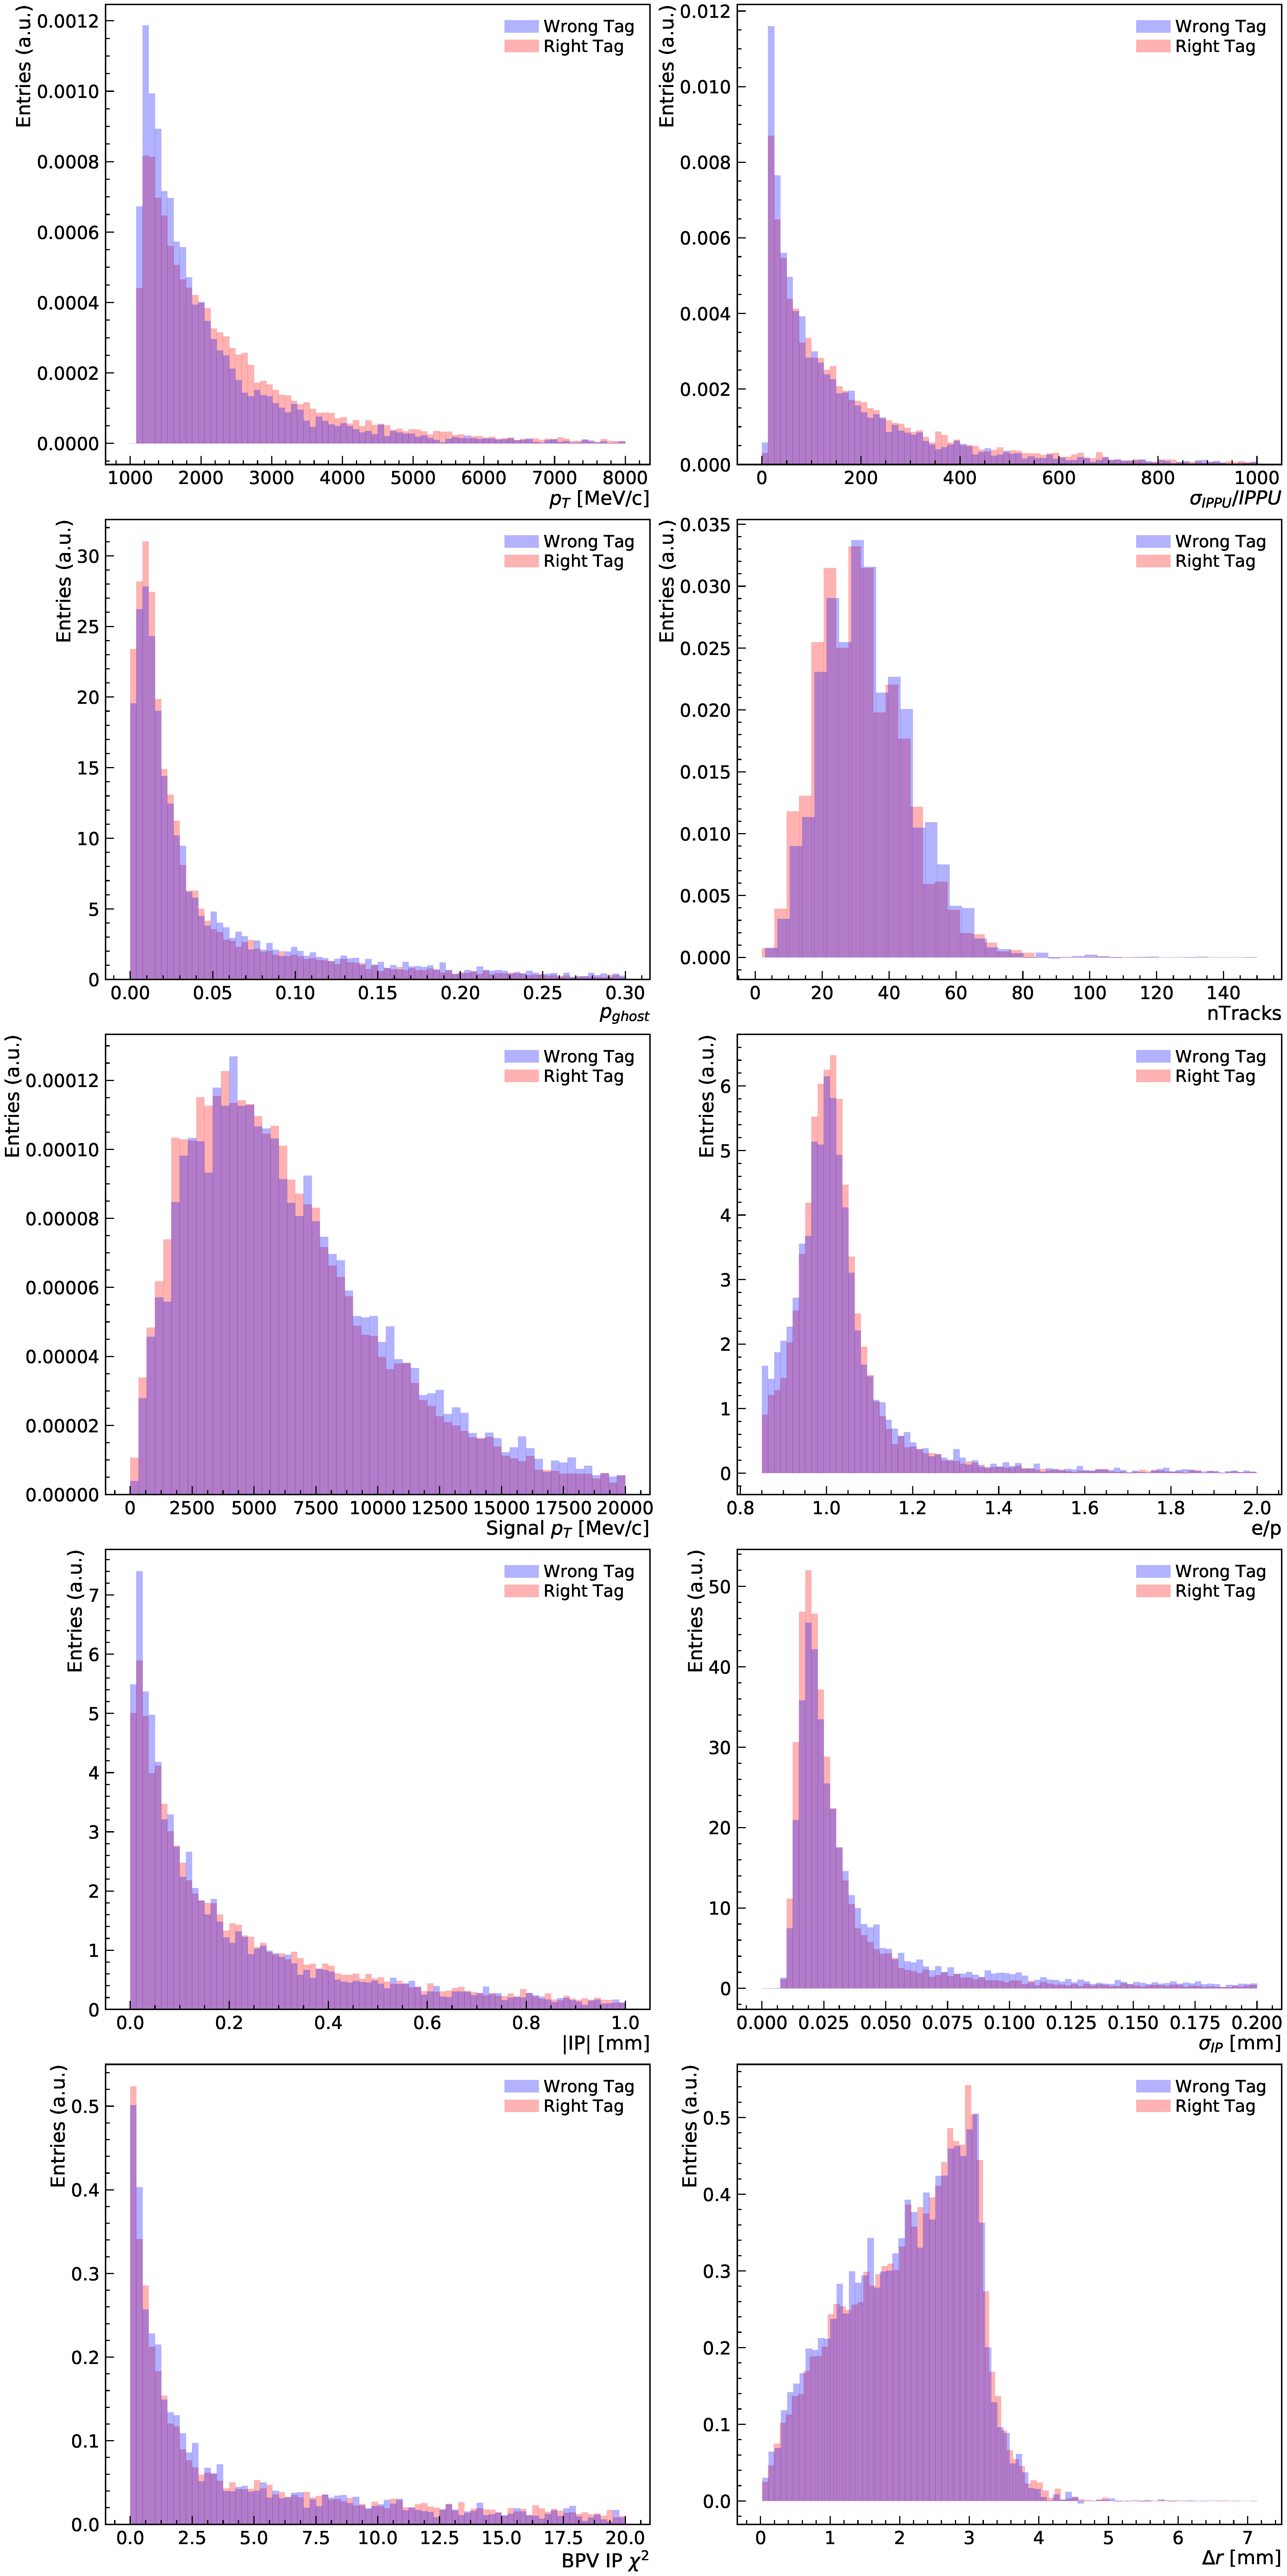
\includegraphics[width=0.7\textwidth]{04Flavourtagging/figs/OSelectronOpt/2017-12-12-vibattis-OSElectron-bdt-calibration-sWeights_Run1/FeaturesDistribution_RunIcuts.pdf}
        \end{center}
        \vspace{-2mm}
        \caption{Distributions (for the \emph{sWeighted}, Run 1 $B^+\to J/\psi K^+$ sample) of the input features of the BDT classifier, for candidates with a right (red) and wrong (blue) decision from the \OSe~tagger.}
         \label{fig:OSefeaturesRunI}
\end{figure}

\begin{figure}[htbp]
        \begin{center}
        \includegraphics[width=0.8\textwidth]{04Flavourtagging/figs/OSelectronOpt/2017-12-12-vibattis-OSElectron-bdt-calibration-sWeights_Run2/FeaturesDistribution_RunIIcuts.pdf}
        \end{center}
        \vspace{-2mm}
         \caption{Distributions (for the \emph{sWeighted}, Run 2 $B^+\to J/\psi K^+$ sample) of the input features of the BDT classifier, for candidates with a right (red) and wrong (blue) decision from the \OSe~tagger.}
         \label{fig:OSefeaturesRunIIB2CC}
\end{figure}

\begin{figure}[htbp]
        \begin{center}
        \includegraphics[width=0.8\textwidth]{04Flavourtagging/figs/OSelectronOpt/2018-04-07-vibattis-OSElectron-bdt-calibration-sWeights_Run2_Bu2D0pi/FeaturesDistribution_RunIIcuts.pdf}
        \end{center}
        \vspace{-2mm}
        \caption{Distributions (for the \emph{sWeighted}, Run 2 $B^+\to D^0 \pi^+$ sample) of the input features of the BDT classifier, for candidates with a right (red) and wrong (blue) decision from the \OSe~tagger.}
         \label{fig:OSefeaturesRunIIB2OC}
\end{figure}

\begin{figure}[htbp]
        \begin{center}
        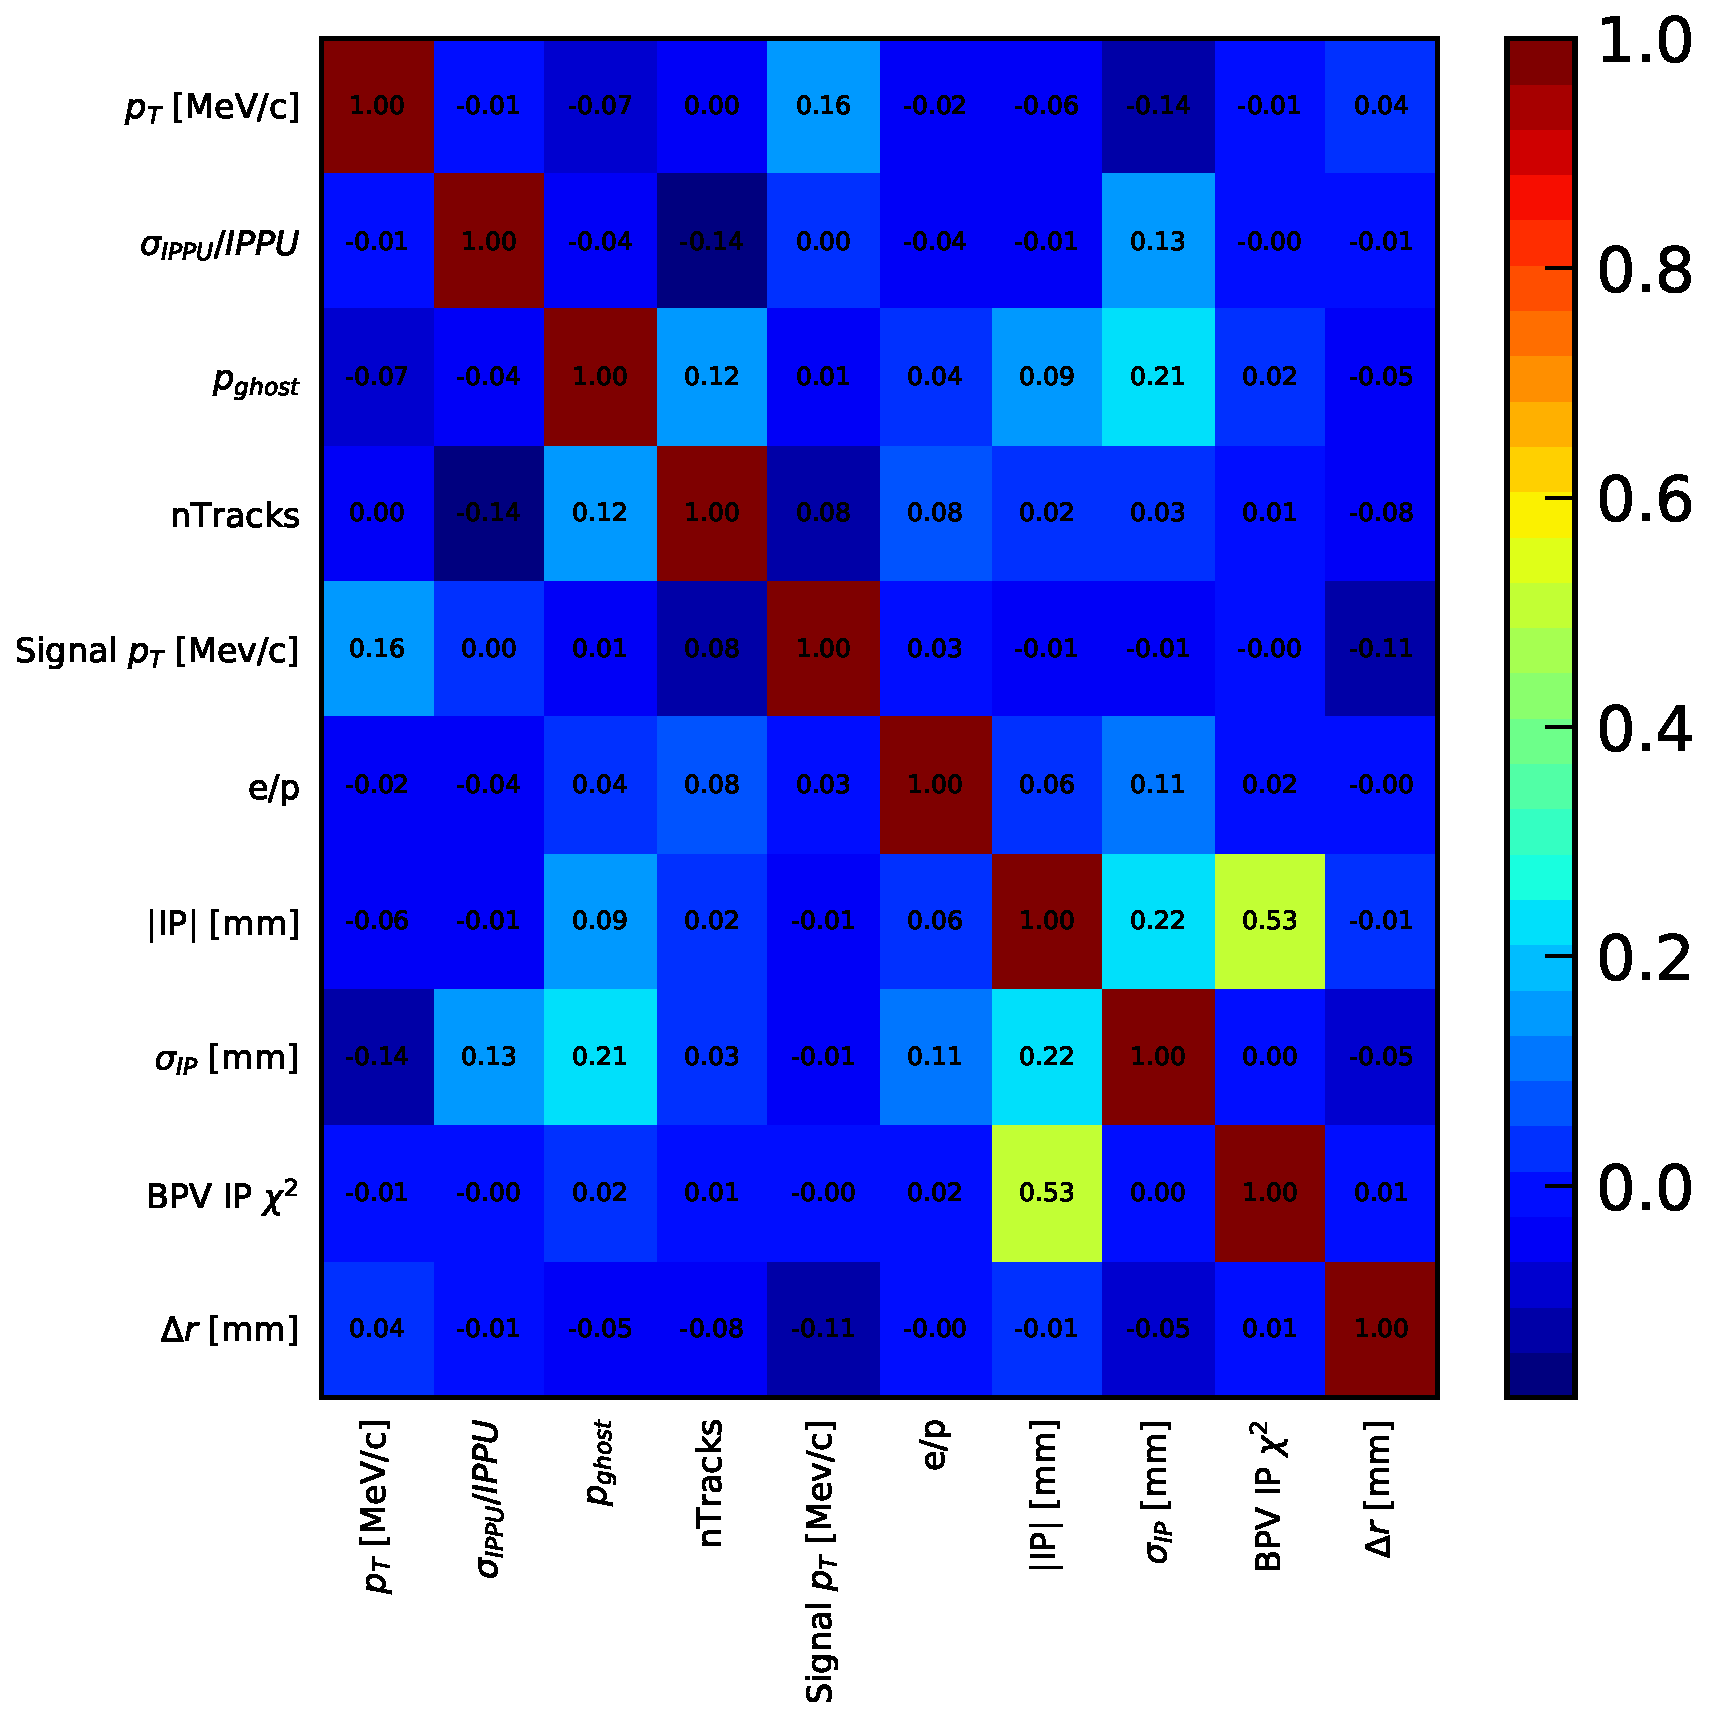
\includegraphics[width=0.47\textwidth]{04Flavourtagging/figs/OSelectronOpt/2017-12-12-vibattis-OSElectron-bdt-calibration-sWeights_Run1/FeaturesCorrRightTag_RunIcuts.pdf}
        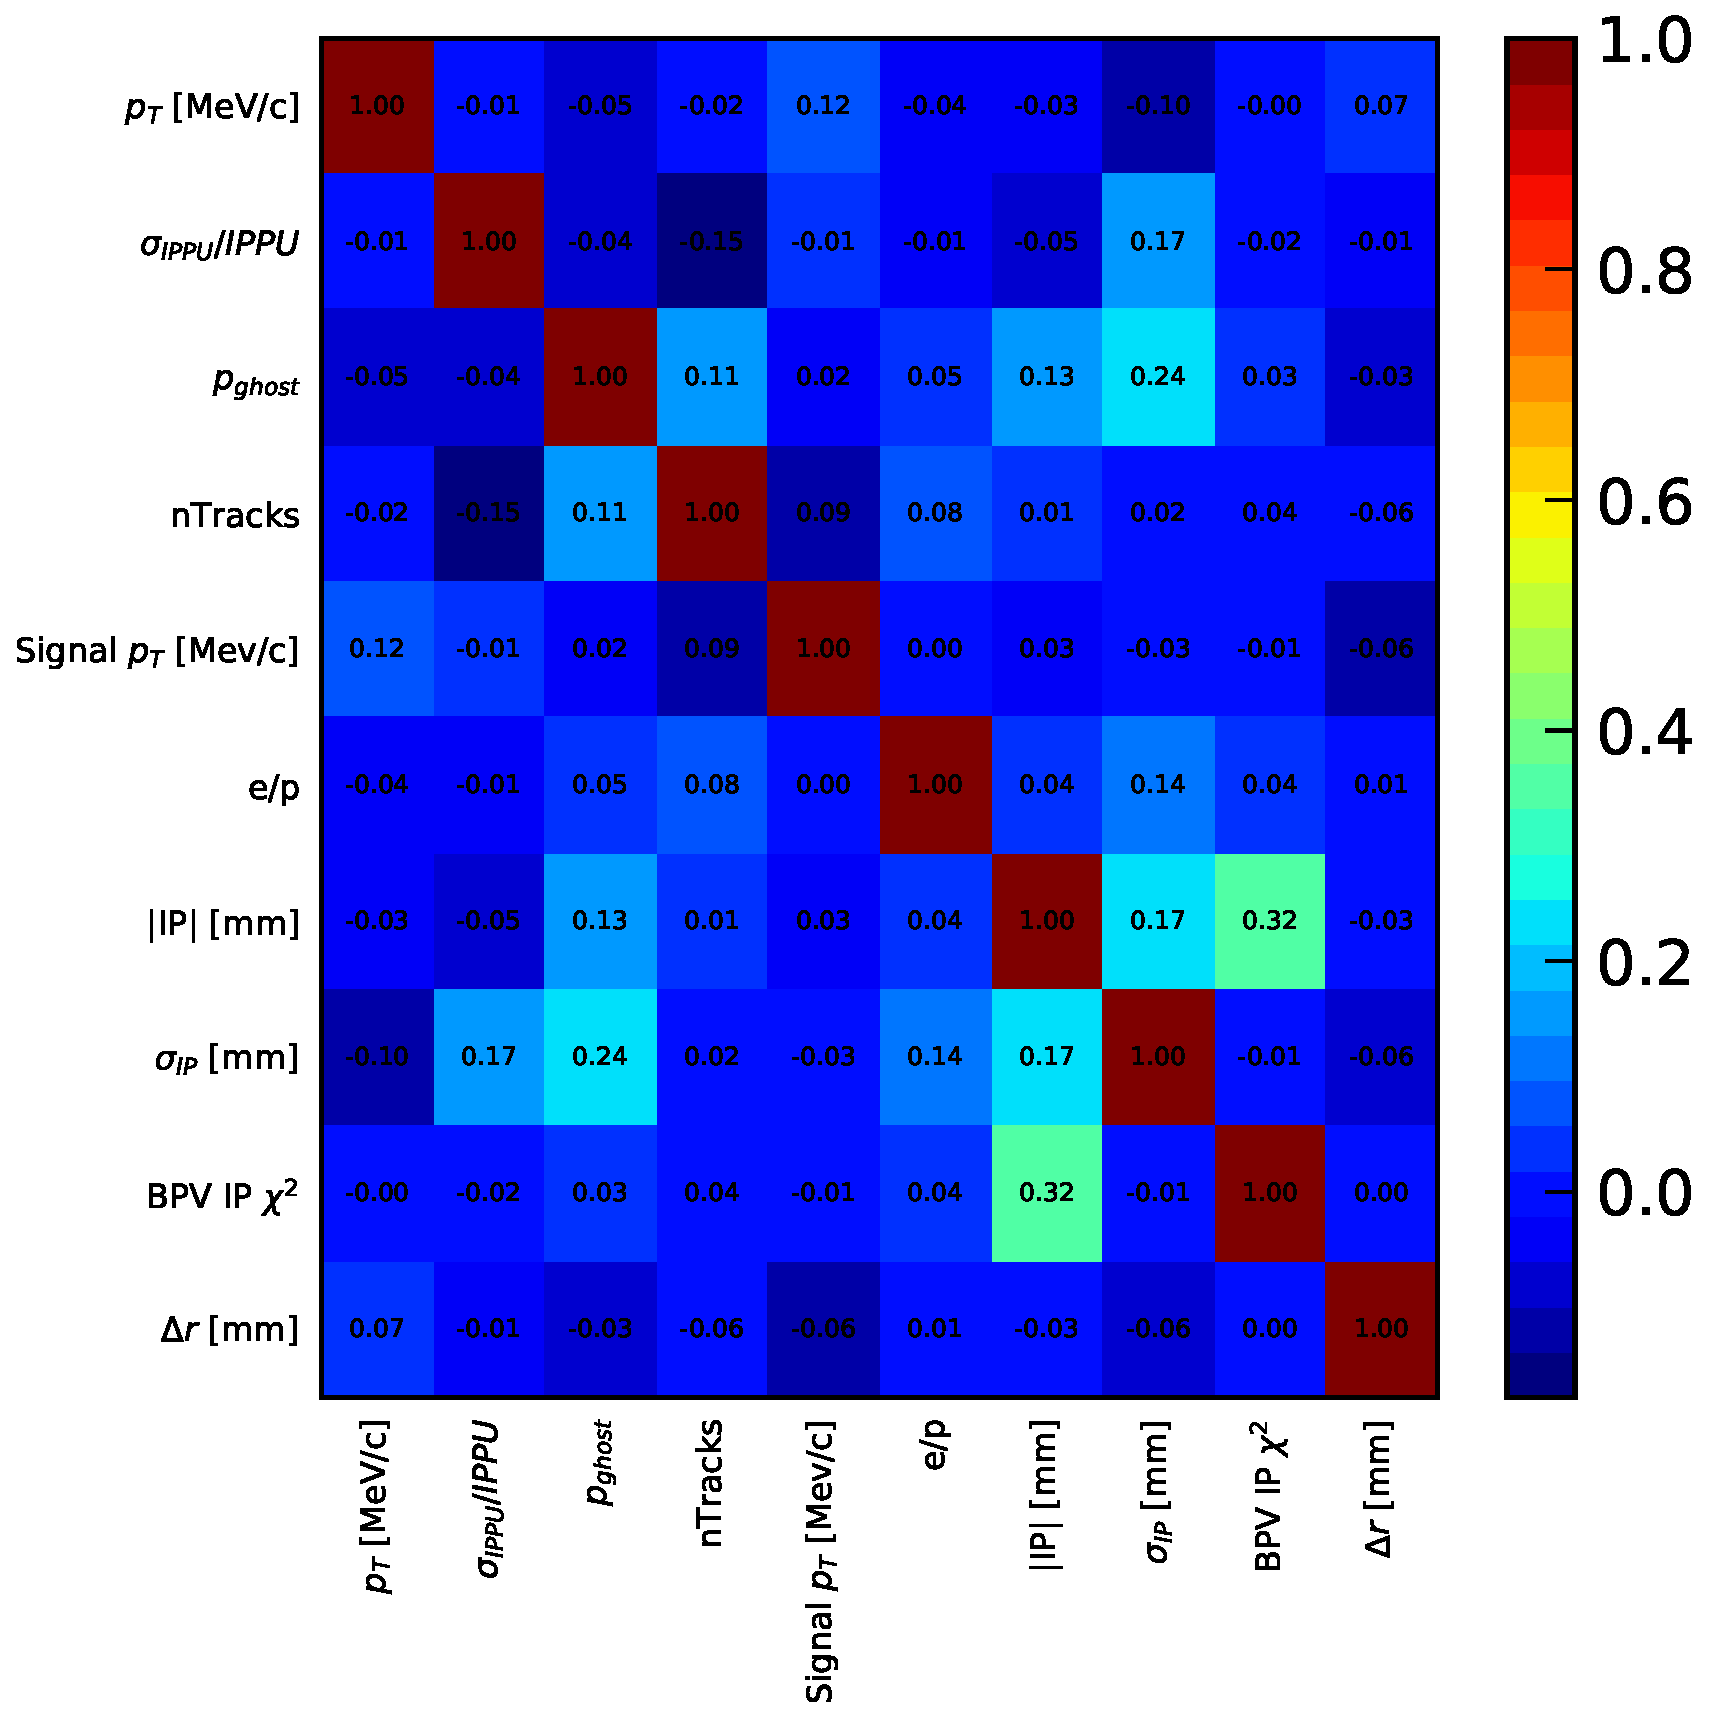
\includegraphics[width=0.47\textwidth]{04Flavourtagging/figs/OSelectronOpt/2017-12-12-vibattis-OSElectron-bdt-calibration-sWeights_Run1/FeaturesCorrWrongTag_RunIcuts.pdf} \\
        \includegraphics[width=0.47\textwidth]{04Flavourtagging/figs/OSelectronOpt/2017-12-12-vibattis-OSElectron-bdt-calibration-sWeights_Run2/FeaturesCorrRightTag_RunIIcuts.pdf}
        \includegraphics[width=0.47\textwidth]{04Flavourtagging/figs/OSelectronOpt/2017-12-12-vibattis-OSElectron-bdt-calibration-sWeights_Run2/FeaturesCorrWrongTag_RunIIcuts.pdf} \\
        \includegraphics[width=0.47\textwidth]{04Flavourtagging/figs/OSelectronOpt/2018-04-07-vibattis-OSElectron-bdt-calibration-sWeights_Run2_Bu2D0pi/FeaturesCorrRightTag_RunIIcuts.pdf}
        \includegraphics[width=0.47\textwidth]{04Flavourtagging/figs/OSelectronOpt/2018-04-07-vibattis-OSElectron-bdt-calibration-sWeights_Run2_Bu2D0pi/FeaturesCorrWrongTag_RunIIcuts.pdf} \\
        \end{center}
        \vspace{-2mm}
        \caption{Pearson correlation coefficients between the input features of the Run 1 new (top), Run 2 B2CC (middle) and Run 2 B2OC (bottom) BDT classifiers, for candidates with a correct (left) and wrong (right) decision from the \OSe~tagger.}
         \label{fig:OSecorrelations}
\end{figure}

The BDT classifier consists of an ensemble of 300 gradient-boosted decision trees~\cite{xgboost}, where each tree can have a maximum depth of 3. The objective of the classifier is a binary logistic loss function plus a quadratic regularisation term to control model complexity (with regularisation parameter $\lambda=1$). Some hyperparameters were tested by means of a cross-validation+bootstrapping method on the training set, as described in Appendix~\ref{app:oselectronappendix}. The importance (or F score) of each feature, defined as the total number of times a feature is chosen as split node by any tree in the BDT ensemble, is presented in Fig.~\ref{fig:OSeimportance}, while the \emph{partial dependence} of the predicted mistag $\eta$ (on the training set) as a function of each input feature is shown in Appendix~\ref{app:oselectronappendix}. 
The receiver operating characteristic (ROC) curves, which report the \emph{true positive rate}  
as a function of the \emph{false positive rate}, 
are shown in Fig.~\ref{fig:OSerocs}. 
The true (false) positive rate is the fraction of true, correctly (incorrectly) tagged candidates over all candidates classified as correctly tagged. 
The feature selection, BDT training and feature importance evaluation chain is repeated iteratively in order to exclude highly-correlated and poorly-important features, until the BDT performance starts to degrade significantly.

\begin{figure}[t]
        \begin{center}
        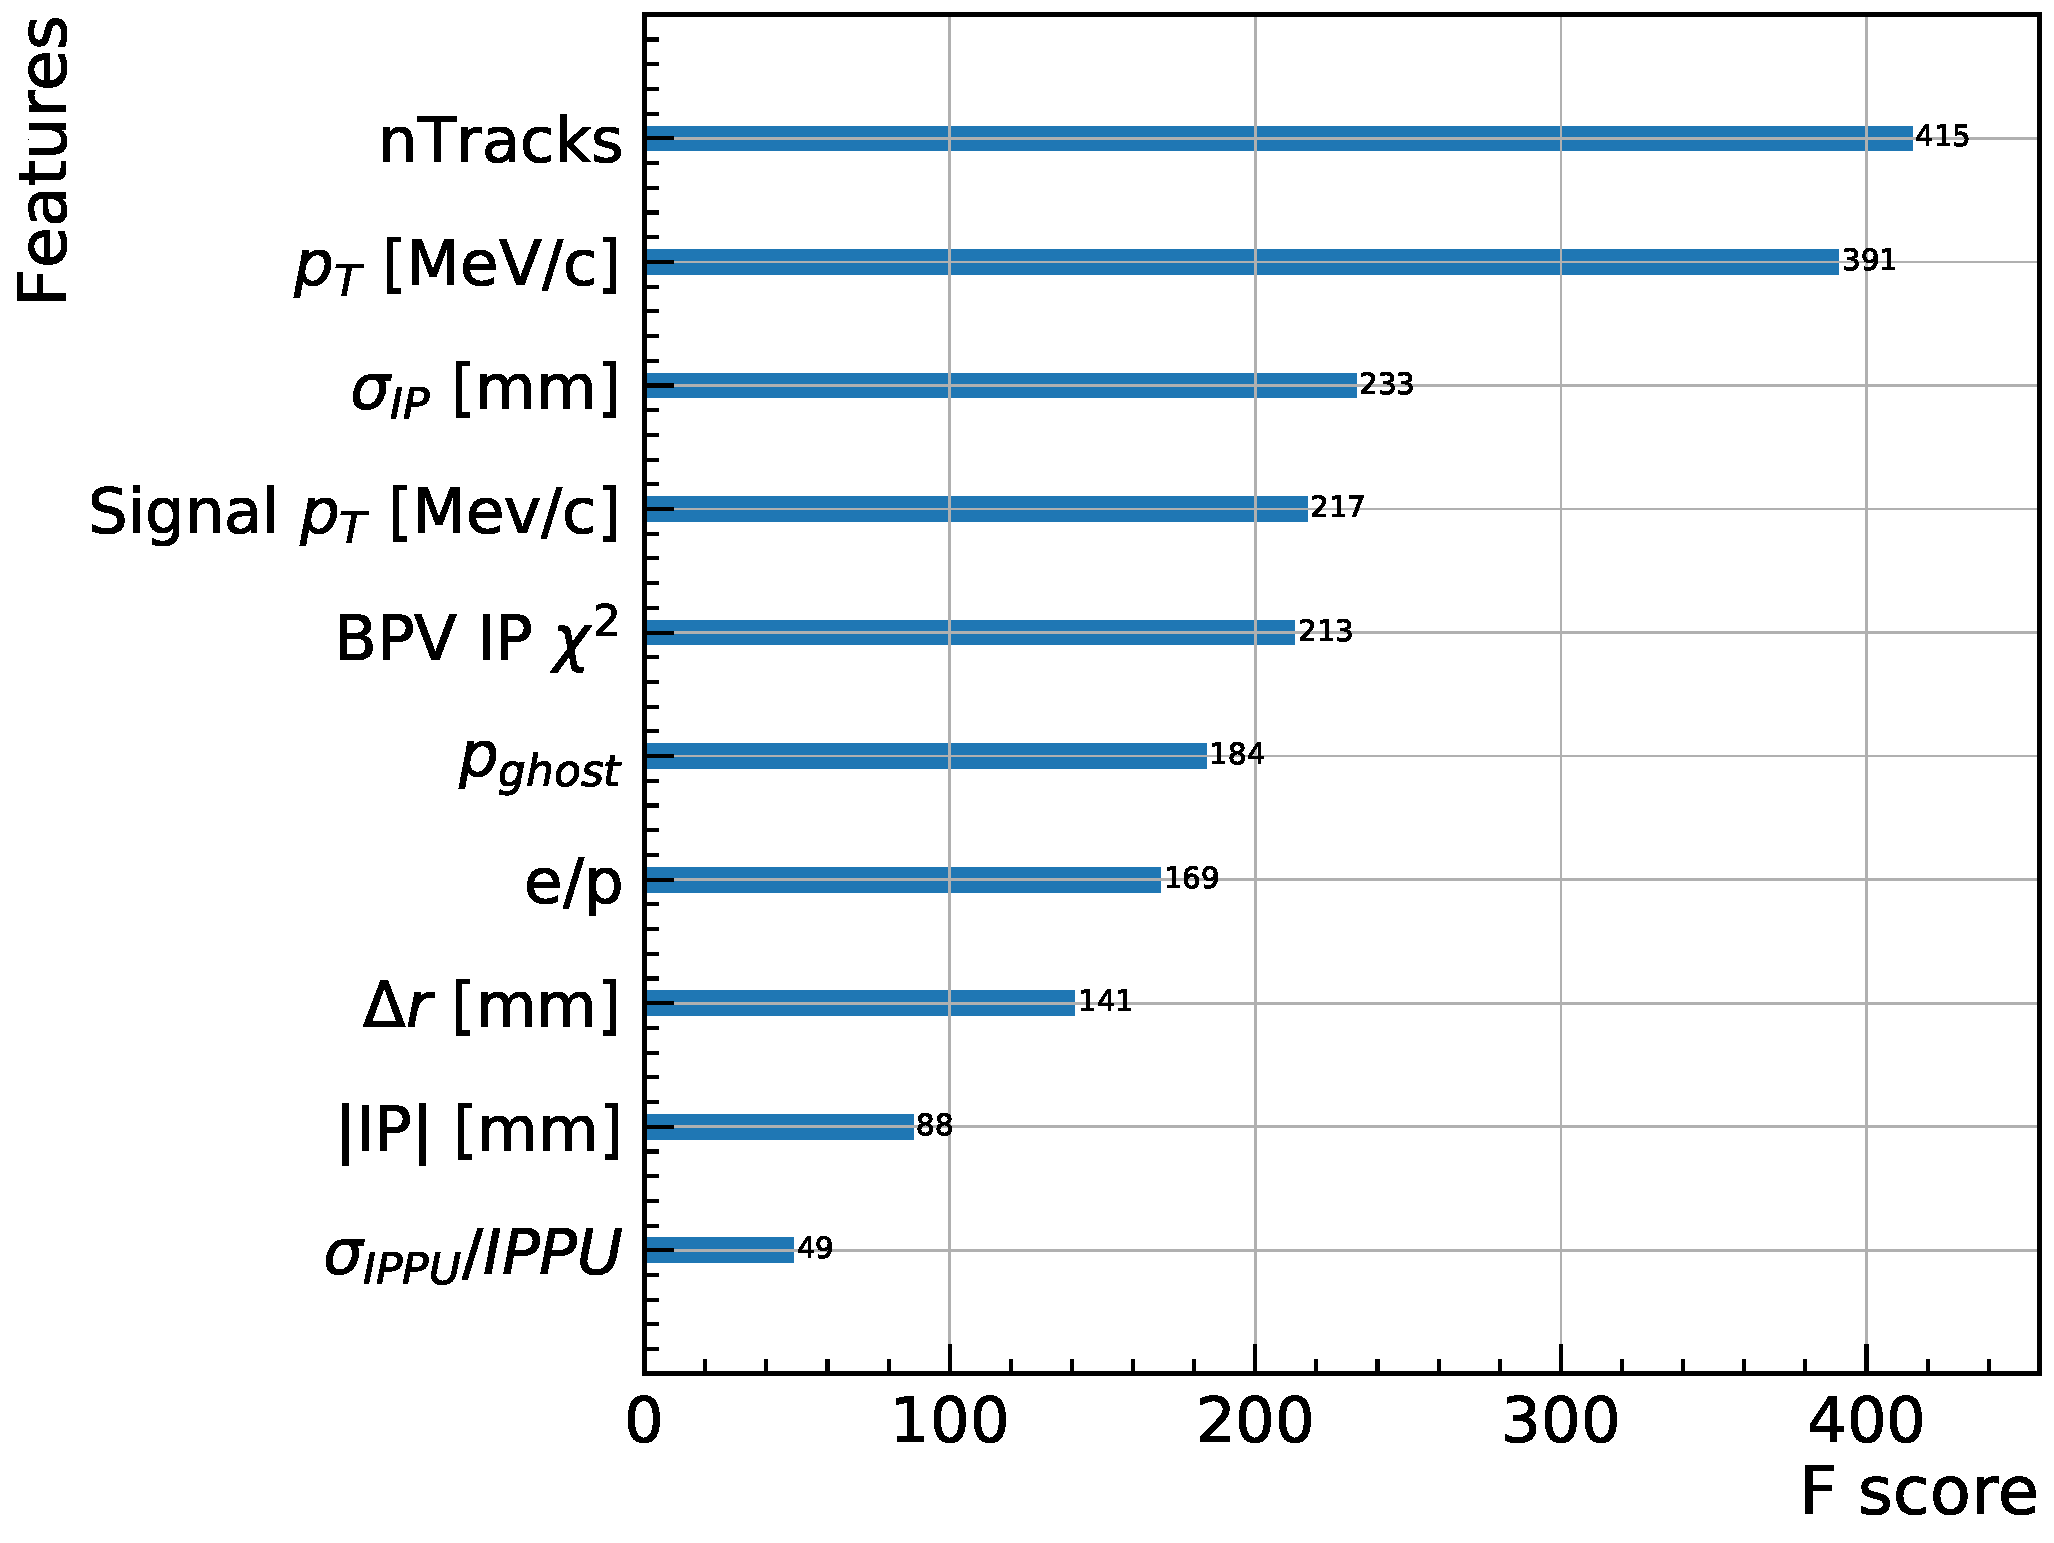
\includegraphics[width=0.4\textwidth]{04Flavourtagging/figs/OSelectronOpt/2017-12-12-vibattis-OSElectron-bdt-calibration-sWeights_Run1/Importance_RunIcuts.pdf}
        \includegraphics[width=0.4\textwidth]{04Flavourtagging/figs/OSelectronOpt/2017-12-12-vibattis-OSElectron-bdt-calibration-sWeights_Run2/Importance_RunIIcuts.pdf} \\
        \includegraphics[width=0.4\textwidth]{04Flavourtagging/figs/OSelectronOpt/2018-04-07-vibattis-OSElectron-bdt-calibration-sWeights_Run2_Bu2D0pi/Importance_RunIIcuts.pdf}
        \end{center}
        \vspace{-2mm}
        \caption{Feature importance for the BDT classifiers of the Run 1 new (top left), Run 2 B2CC (top right) and Run 2 B2OC (bottom) implementations of the \OSe~tagger.}
         \label{fig:OSeimportance}
\end{figure}

\begin{figure}[t]
        \begin{center}
        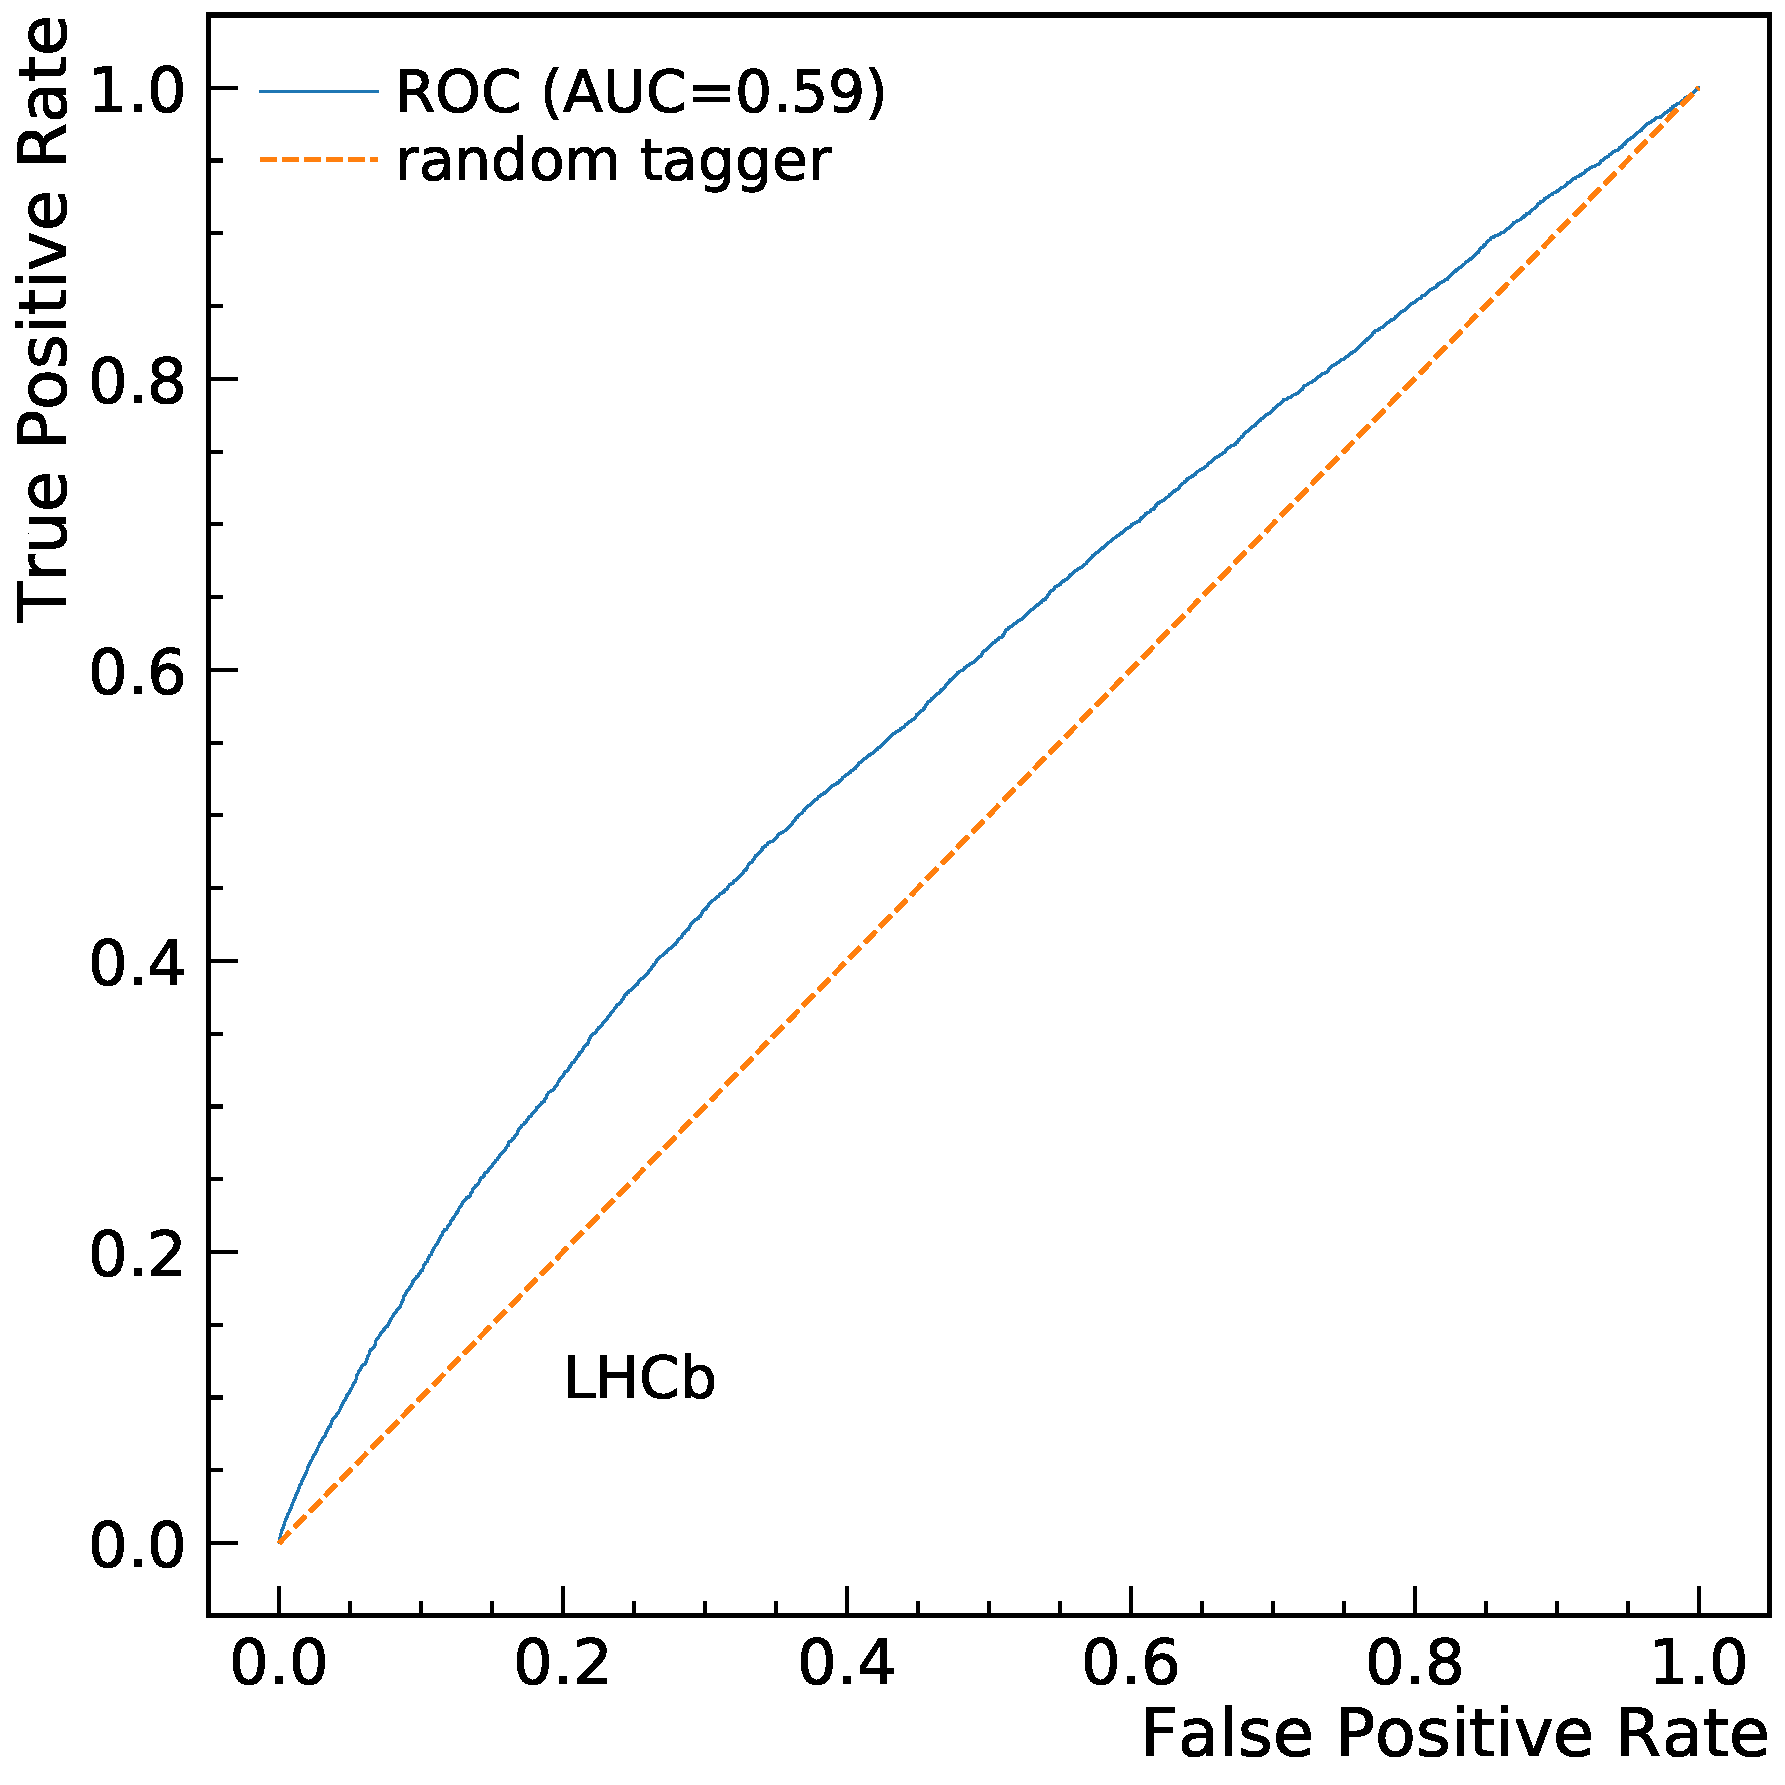
\includegraphics[width=0.4\textwidth]{04Flavourtagging/figs/OSelectronOpt/2017-12-12-vibattis-OSElectron-bdt-calibration-sWeights_Run1/ROC_RunIcuts.pdf}
        \includegraphics[width=0.4\textwidth]{04Flavourtagging/figs/OSelectronOpt/2017-12-12-vibattis-OSElectron-bdt-calibration-sWeights_Run2/ROC_RunIIcuts.pdf} \\
        \includegraphics[width=0.4\textwidth]{04Flavourtagging/figs/OSelectronOpt/2018-04-07-vibattis-OSElectron-bdt-calibration-sWeights_Run2_Bu2D0pi/ROC_RunIIcuts.pdf}
        \end{center}
        \vspace{-2mm}
        \caption{True positive rate as a function of the false positive rate (ROC curves) for the BDT classifiers of the Run 1 new (top left), Run 2 B2CC (top right) and Run 2 B2OC (bottom) implementations of \OSe. The obtained ROC curves are represented in blue, while the expected ROC curve in case of random tag decision is shown as a dashed orange line. For each BDT, the \emph{Area Under the} ROC \emph{Curve} (AUC score) is reported as well.}
         \label{fig:OSerocs}
\end{figure}

For each candidate, the BDT predicts the probability $P$ that such candidates is correctly tagged. In order to obtain a mistag probability $\eta$, the following transformation is applied on both $P$ and tagging decision $d$:
\begin{equation}
        (\eta, d) \rightarrow \begin{cases} (P, -d) &\text{if $P\leq0.5$} \\ (1-P, d) &\text{otherwise} \end{cases}        
\end{equation} 
The distributions of $\eta$ for training and test samples, splitted per target value, are shown in Fig.~\ref{fig:OSeetapredict}.

\begin{figure}[t]
        \begin{center}
        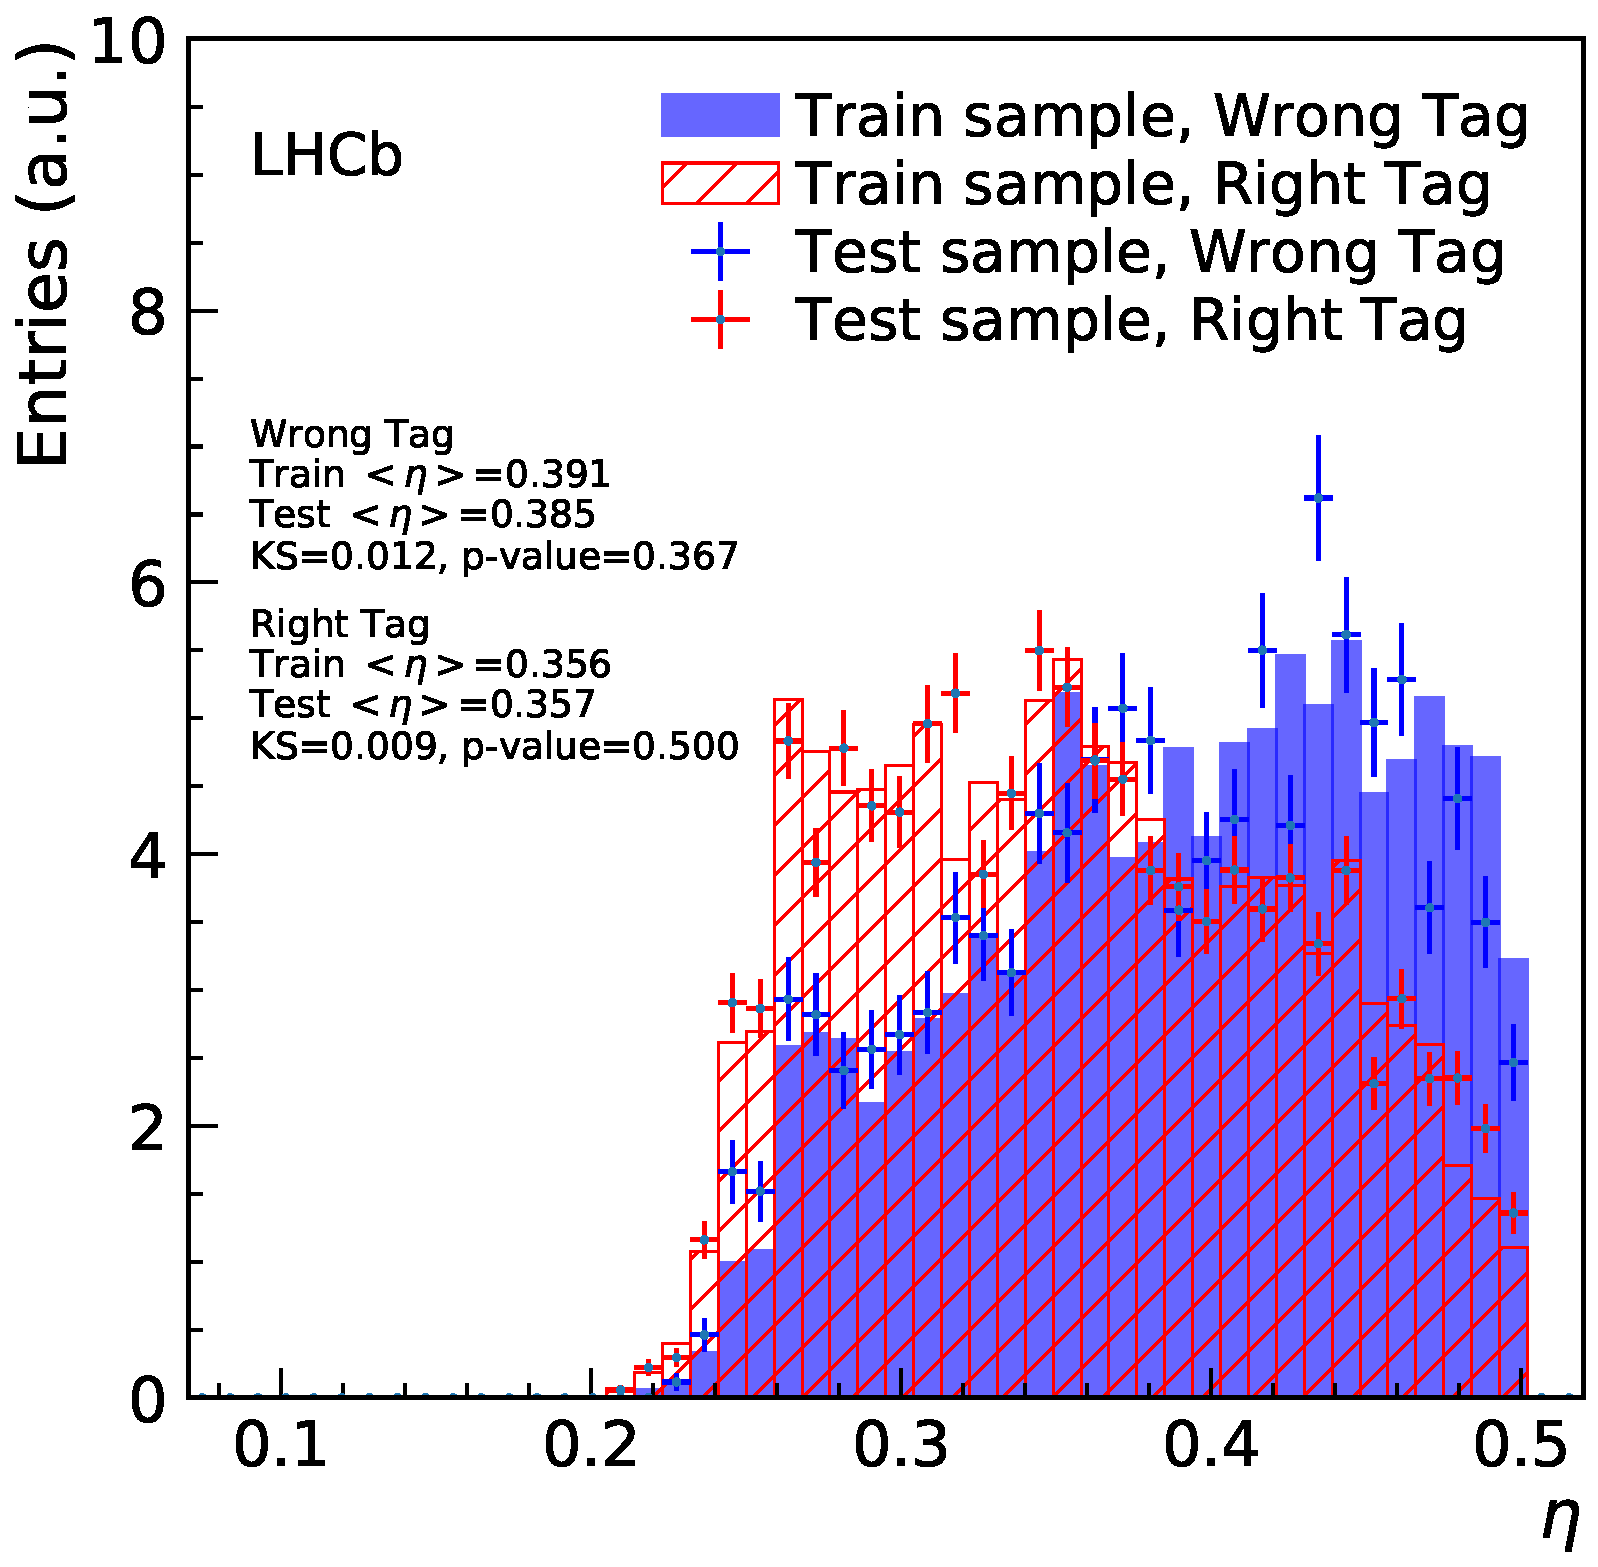
\includegraphics[width=0.4\textwidth]{04Flavourtagging/figs/OSelectronOpt/2017-12-12-vibattis-OSElectron-bdt-calibration-sWeights_Run1/PredictedEta_RunIcuts.pdf}
        \includegraphics[width=0.4\textwidth]{04Flavourtagging/figs/OSelectronOpt/2017-12-12-vibattis-OSElectron-bdt-calibration-sWeights_Run2/PredictedEta_RunIIcuts.pdf}
        \includegraphics[width=0.4\textwidth]{04Flavourtagging/figs/OSelectronOpt/2018-04-07-vibattis-OSElectron-bdt-calibration-sWeights_Run2_Bu2D0pi/PredictedEta_RunIIcuts.pdf}
        \end{center}
        \vspace{-2mm}
        \caption{\emph{sWeighted} distributions of the mistag probability $\eta$ predicted by the BDT classifiers of the Run 1 new (top left), Run 2 B2CC (top right) and Run 2 B2OC (bottom) versions of the \OSe~tagger. 
          The blue-solid (red-hatched) histogram represents the training data for candidates having the wrong (right) tag decision. 
          The blue (red) points indicate the test data for candidates with wrong (right) tag decision. 
          The overtraining is checked, separately for candidates with wrong and right tag decision,
          by means of a Kologorov-Smirnov (KS) test to measure the compatibility between training data and test data.
          The conventional value of $0.05$ is chosen as significance level to reject the hypothesis of compatibility.}
        \label{fig:OSeetapredict}
\end{figure}

%%%%%%%%%%%%%%%%%%%%%%%%%%%%%%%%%%%%%%%%%%%%%%%%%%%%

\subsection{Performance evaluation}

%%%%%%%%%%%%%%%%%%%%%%%%%%%%%%%%%%%%%%%%%%%%%%%%%%%%

\subsubsection[Performance on $B^+\to J/\psi K^+$ and $B^+\to D^0 \pi^+$ data]{Performance on \boldmath{$B^+\to J/\psi K^+$} and \boldmath{$B^+\to D^0 \pi^+$} data}
\label{sec:tagging:OSePerf1}

Once the BDT is trained on the training ssample, the mistag $\eta$ is predicted for each candidate using the evaluation samples. Then, a two-fold evaluation is applied:
\begin{itemize}[noitemsep,topsep=0pt]
        \item the mistag calibration is determined on the first evaluation sample. The obtained calibration is then applied to the second evaluation sample, and a calibrated per-event tagging power is computed on the latter;
        \item same as above, but with the two evaluation samples swapped.
\end{itemize}
The calibrated per-event tagging power is computed by considering, for each tagged $B$ candidate, only the tagging particle with the highest transverse momentum.
The calibration model consists of a first order natural spline with a logistic link function.
The result of these calibrations are shown in Fig.~\ref{fig:OSeetacalib}.
The calibrated per-event tagging power is reported in Table~\ref{tab:OSeperformanceevalset}.

\begin{figure}[t]
        \begin{center}
        \includegraphics[width=0.4\textwidth]{04Flavourtagging/figs/OSelectronOpt/RunIEval_Bu2JpsiKst/eval_on_I.pdf}
        \includegraphics[width=0.4\textwidth]{04Flavourtagging/figs/OSelectronOpt/RunIEval_Bu2JpsiKst/eval_on_II.pdf} \\
        \includegraphics[width=0.4\textwidth]{04Flavourtagging/figs/OSelectronOpt/RunIIEval_Bu2JpsiKst/eval_on_I.pdf}
        \includegraphics[width=0.4\textwidth]{04Flavourtagging/figs/OSelectronOpt/RunIIEval_Bu2JpsiKst/eval_on_II.pdf} \\
        \includegraphics[width=0.4\textwidth]{04Flavourtagging/figs/OSelectronOpt/RunIIEval_Bu2D0Pi/eval_on_I.pdf}
        \includegraphics[width=0.4\textwidth]{04Flavourtagging/figs/OSelectronOpt/RunIIEval_Bu2D0Pi/eval_on_II.pdf}
        \end{center}
        \vspace{-2mm}
        \caption{\OSe~mistag calibration results for the (top) Run 1 new, (middle) Run 2 B2CC and (bottom) Run 2 B2OC optimisations. Left: calibration obtained on the second evaluation sample plotted together with the first evaluation sample. Right: calibration obtained on the first evaluation sample plotted together with the second evaluation sample. The \emph{sWeighted} data sample is shown as black points. The green (yellow) band indicates the 68\% (95\%) C.L. interval for the fitted calibration functions.}
        \label{fig:OSeetacalib}
\end{figure}

\begin{table}[t]
	\centering
        \caption{Calibrated, per-event tagging power $\effeff$ (in $\%$) of the \OSe~algorithms obtained on the evaluation sets of each \OSe~implementation. The errors include both statistical uncertainty and uncertainties from the calibration procedure. The average is computed by assuming uncorrelated measurements.}
         \label{tab:OSeperformanceevalset}
        \begin{tabular}{llll}
        \toprule
        Algorithm & set 1 & set 2 & average  \\
        \midrule
        Run 1 new & $0.513\pm0.040$ & $0.496\pm0.038$ & $0.504\pm0.028$ \\
        Run 2 B2CC & $0.324\pm0.031$ & $0.364\pm0.033$ & $0.343\pm0.023$ \\
        Run 2 B2OC & $0.455\pm0.043$ & $0.434\pm0.041$ & $0.444\pm0.030$ \\
        \bottomrule
        \end{tabular}
\end{table}

%%%%%%%%%%%%%%%%%%%%%%%%%%%%%%%%%%%%%%%%%%%%%%%%%%%%

\subsubsection[Performance on $B^0\to D^-\pi^+$ data]{Performance on \boldmath{$B^0\to D^-\pi^+$} data}
\label{sec:tagging:OSePerf2}

The performance (tagging efficiency, mistag probability, tagging power) of the calibrated \OSe~tagger is evaluated on Run 1 (2012) and Run 2 (2016) \emph{sWeighted} data samples of $B^0\to D^-\pi^+$ decays.
These decays ensure a robust estimation of the performance thanks to the high statistics collected at LHCb. Moreover, this channel was not exploited in the development of
the \OSe~tagger, so that it constitutes an independent validation of these algorithms. The performance of the other OS taggers (\OSmu, \OSK, \OSc, \OSvtx, and their combination) is presented
as well in this section in order to provide a complete overview.

The calibration and the performance evaluation are done as follows:
\begin{itemize}[noitemsep,topsep=0pt]
  \item each sample (Run 1 and Run 2) is split randomly in two subsamples;
    \item the calibrations are found on one subsample for all OS taggers;
      \item the obtained calibrations are applied to the other subsample, and the calibrated performance is evaluated.
        \item the calibrated OS taggers are combined, the combination is calibrated in order to correct for effects due to correlations among taggers, and the performance of the calibrated combination is evaluated.
\end{itemize}

The calibrations are obtained via a time-dependent analysis of the $B^0\to D^-\pi^+$ decays, where acceptance and resolution effects are neglected as described in Ref.~\cite{EPM}; moreover, the Cabibbo-suppressed decay mode $B^0\to D^+\pi^-$ is ignored as well.
The chosen model 
$\omega(\eta)$ for each tagger is a GLM model with a logistic link function, and a first order spline as basis function. The results of the calibration and the mistag distribution of each \OSe~implementation are shown in Figs.~\ref{fig:OSePerfCalib1} and~\ref{fig:OSePerfCalib3}; the calibration and the mistag of the corresponding OS combinations are also reported in Figs.~\ref{fig:OSePerfCalib2} and~\ref{fig:OSePerfCalib4}.
 
\begin{figure}[ht!]
        \centering
        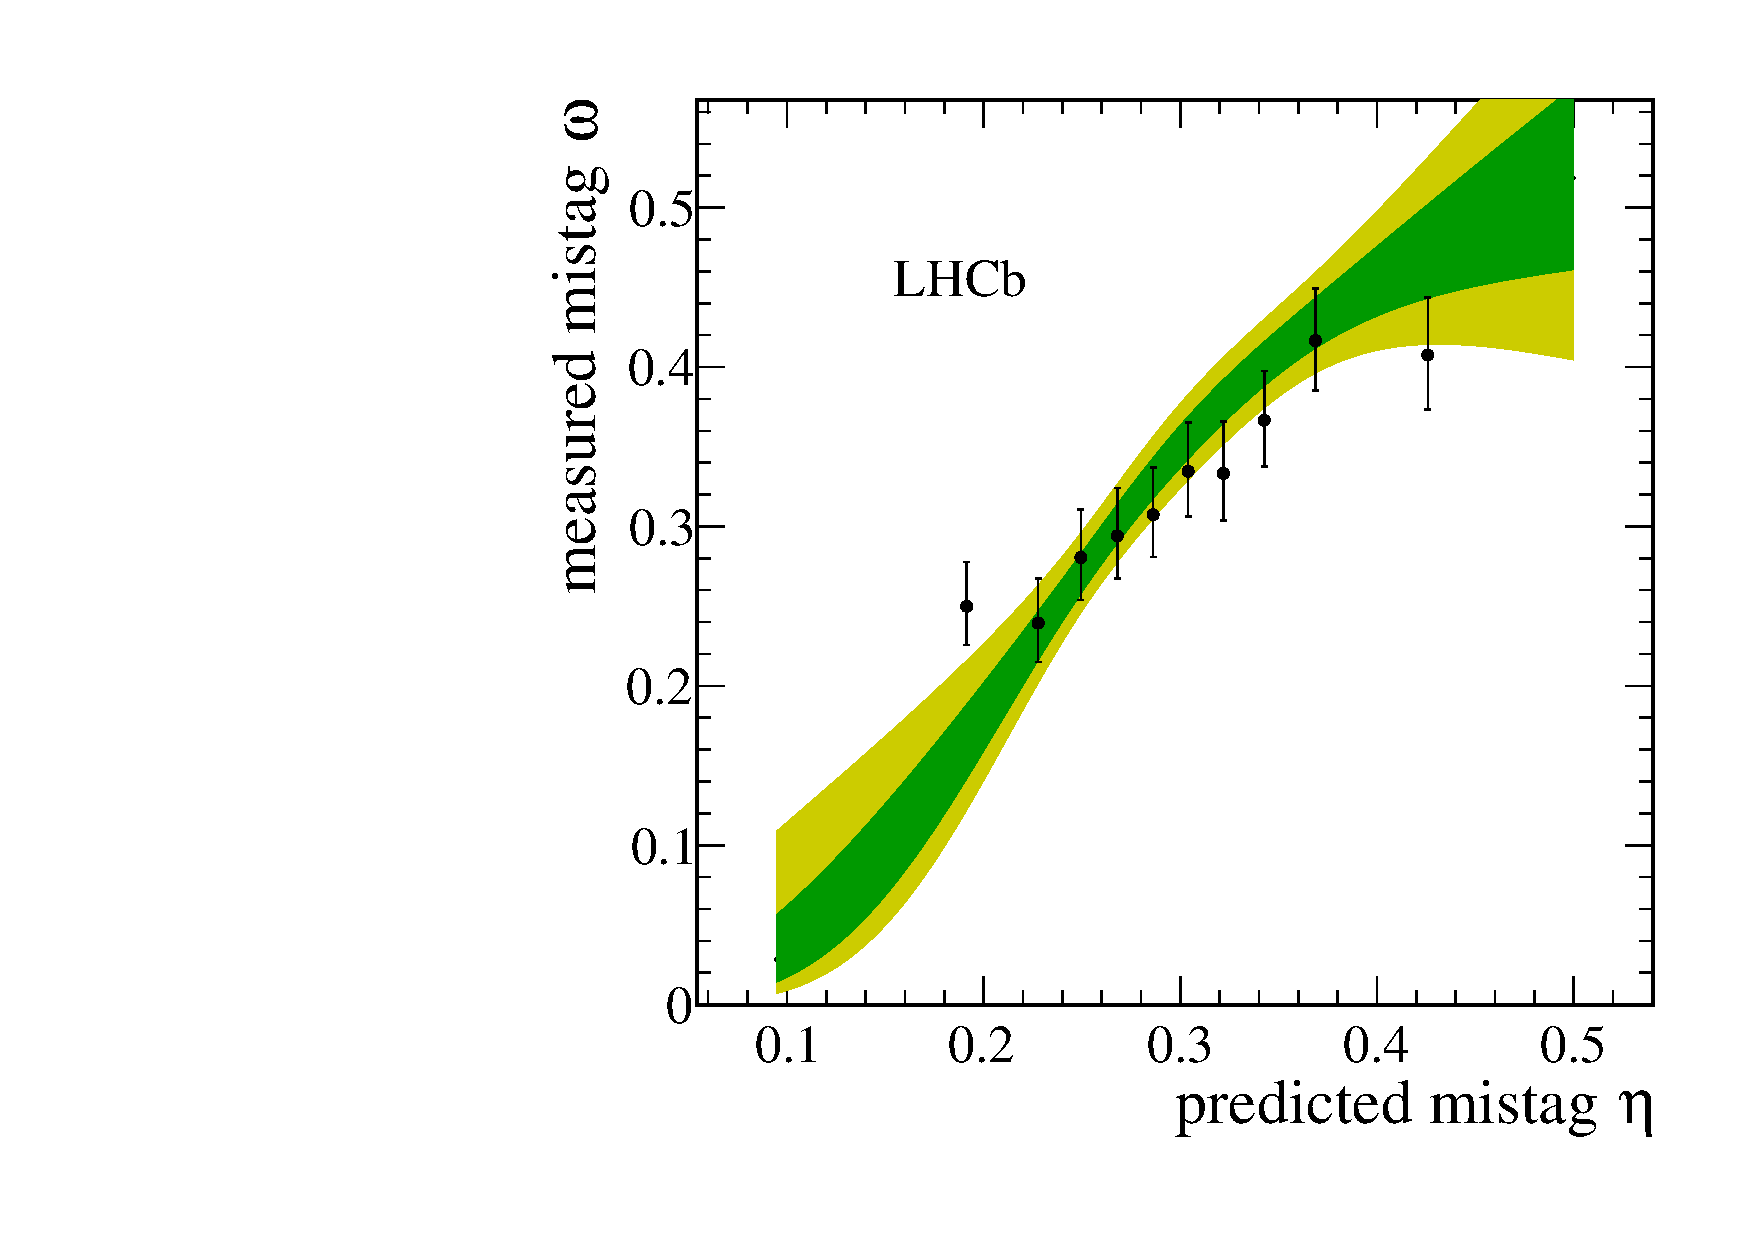
\includegraphics[width=0.26\textwidth]{04FlavourTagging/figs/OSelectronOpt/run1data_old/OS_Electron_InputCalibration.pdf}
        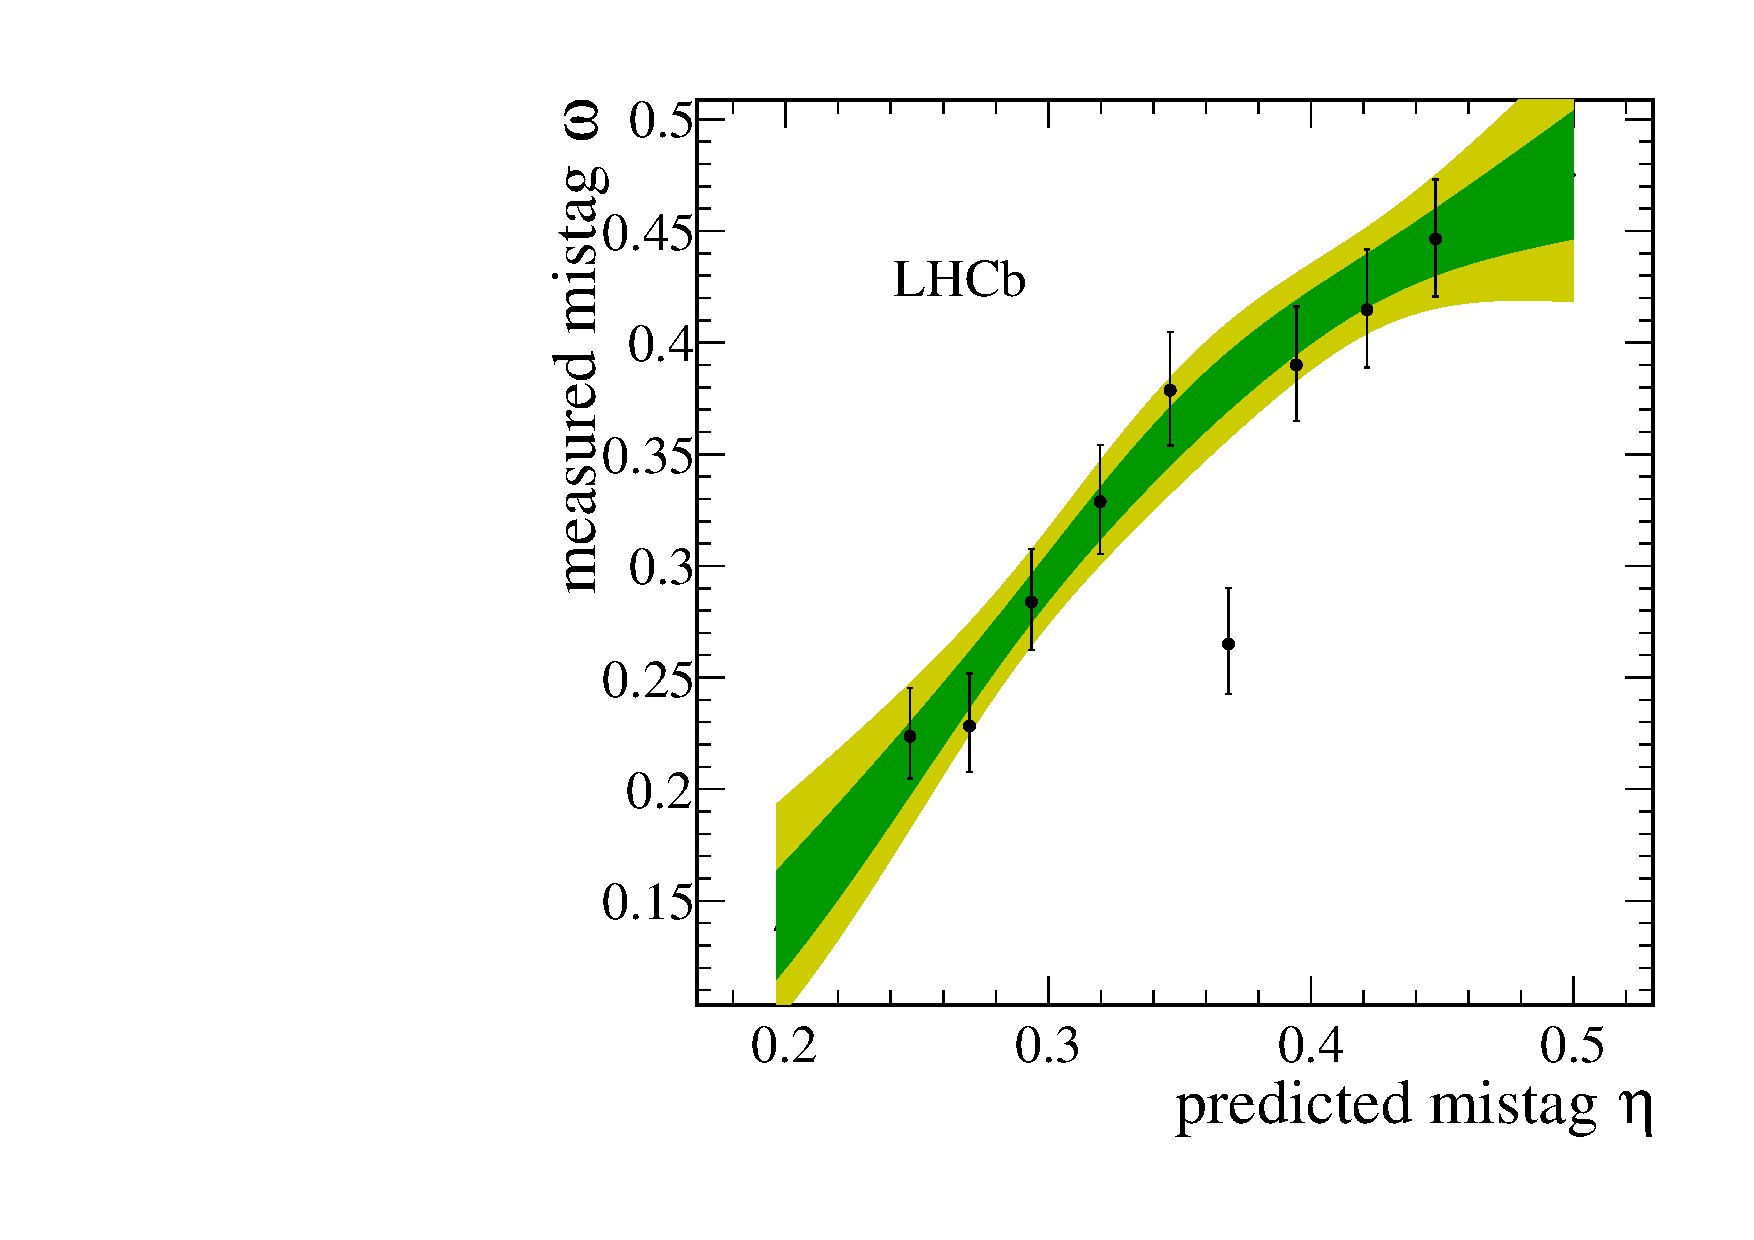
\includegraphics[width=0.26\textwidth]{04FlavourTagging/figs/OSelectronOpt/run1data_new/OS_Electron_InputCalibration.pdf} \\
        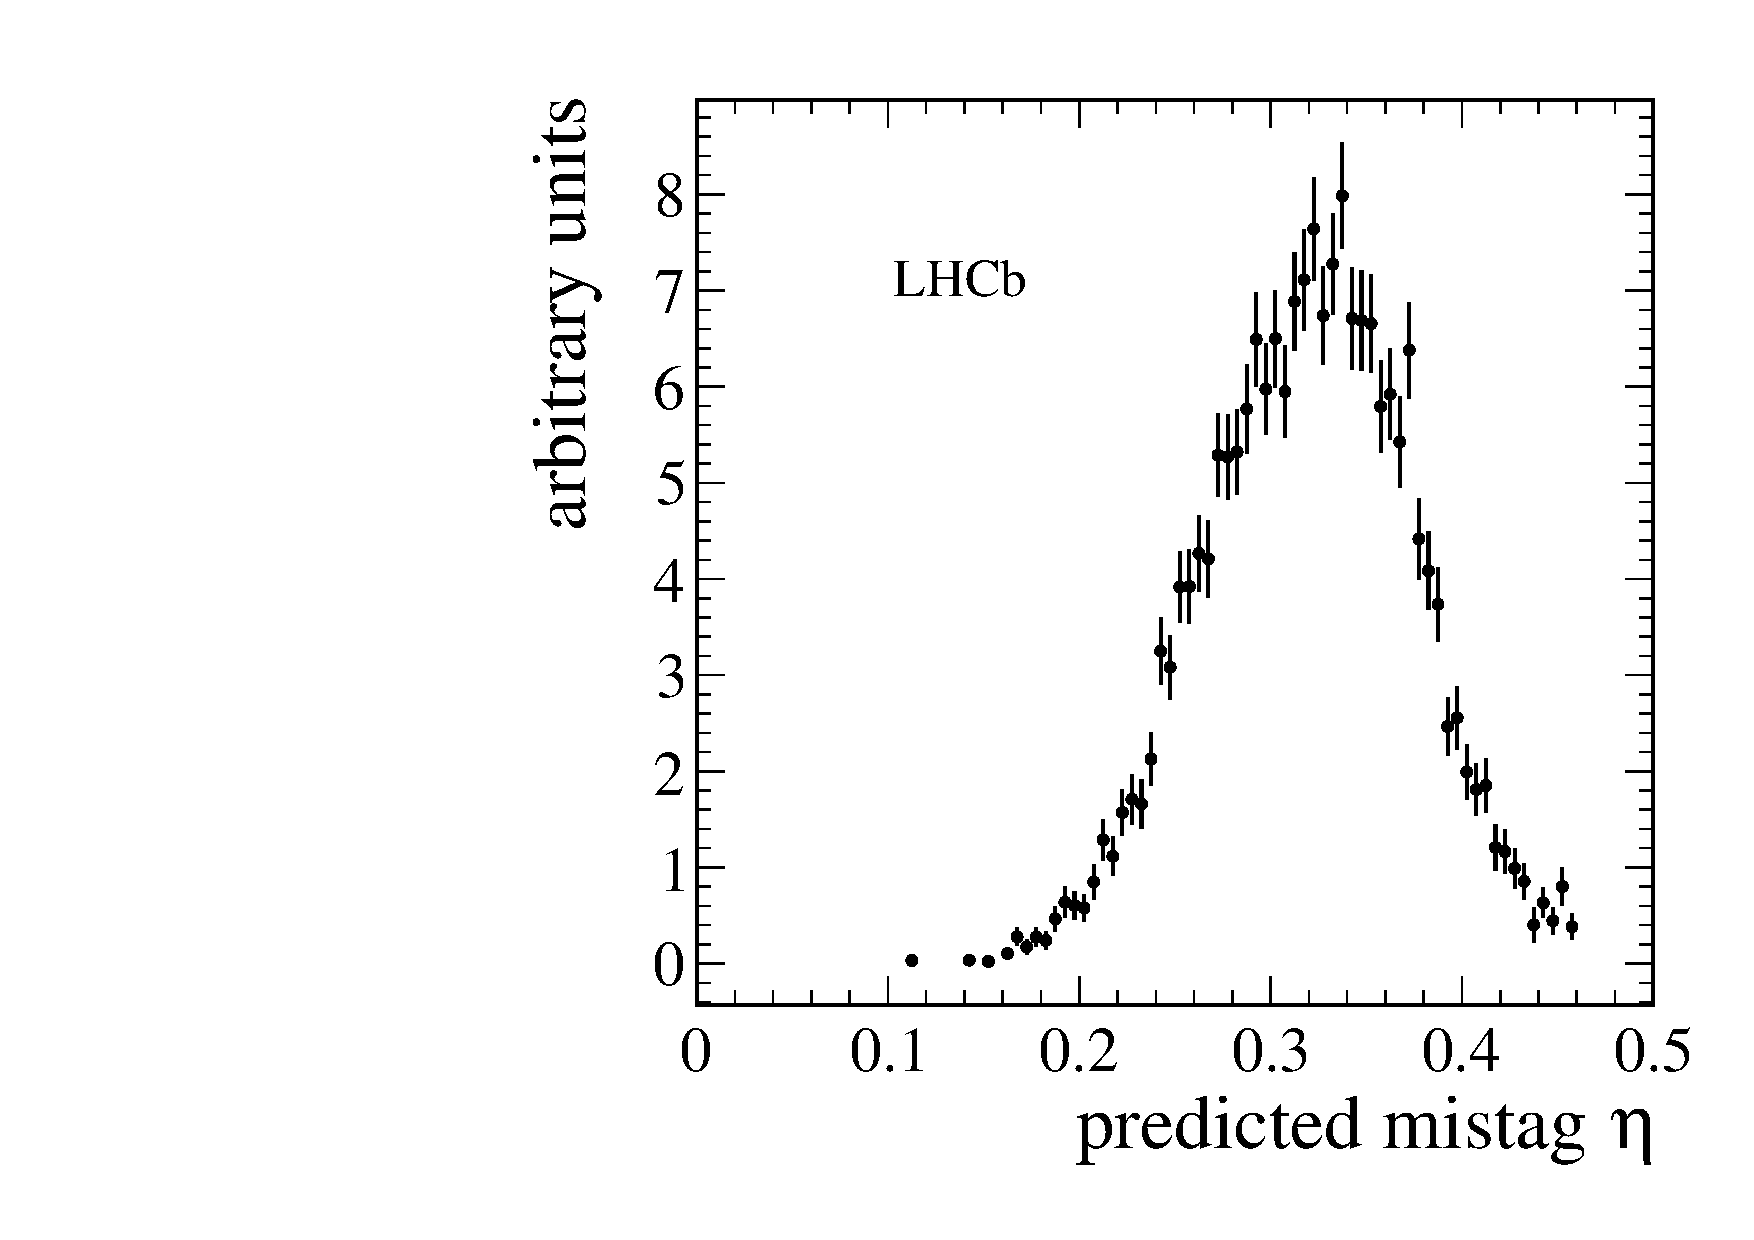
\includegraphics[width=0.26\textwidth]{04FlavourTagging/figs/OSelectronOpt/run1data_old/OS_Electron_EtaDist.pdf}
        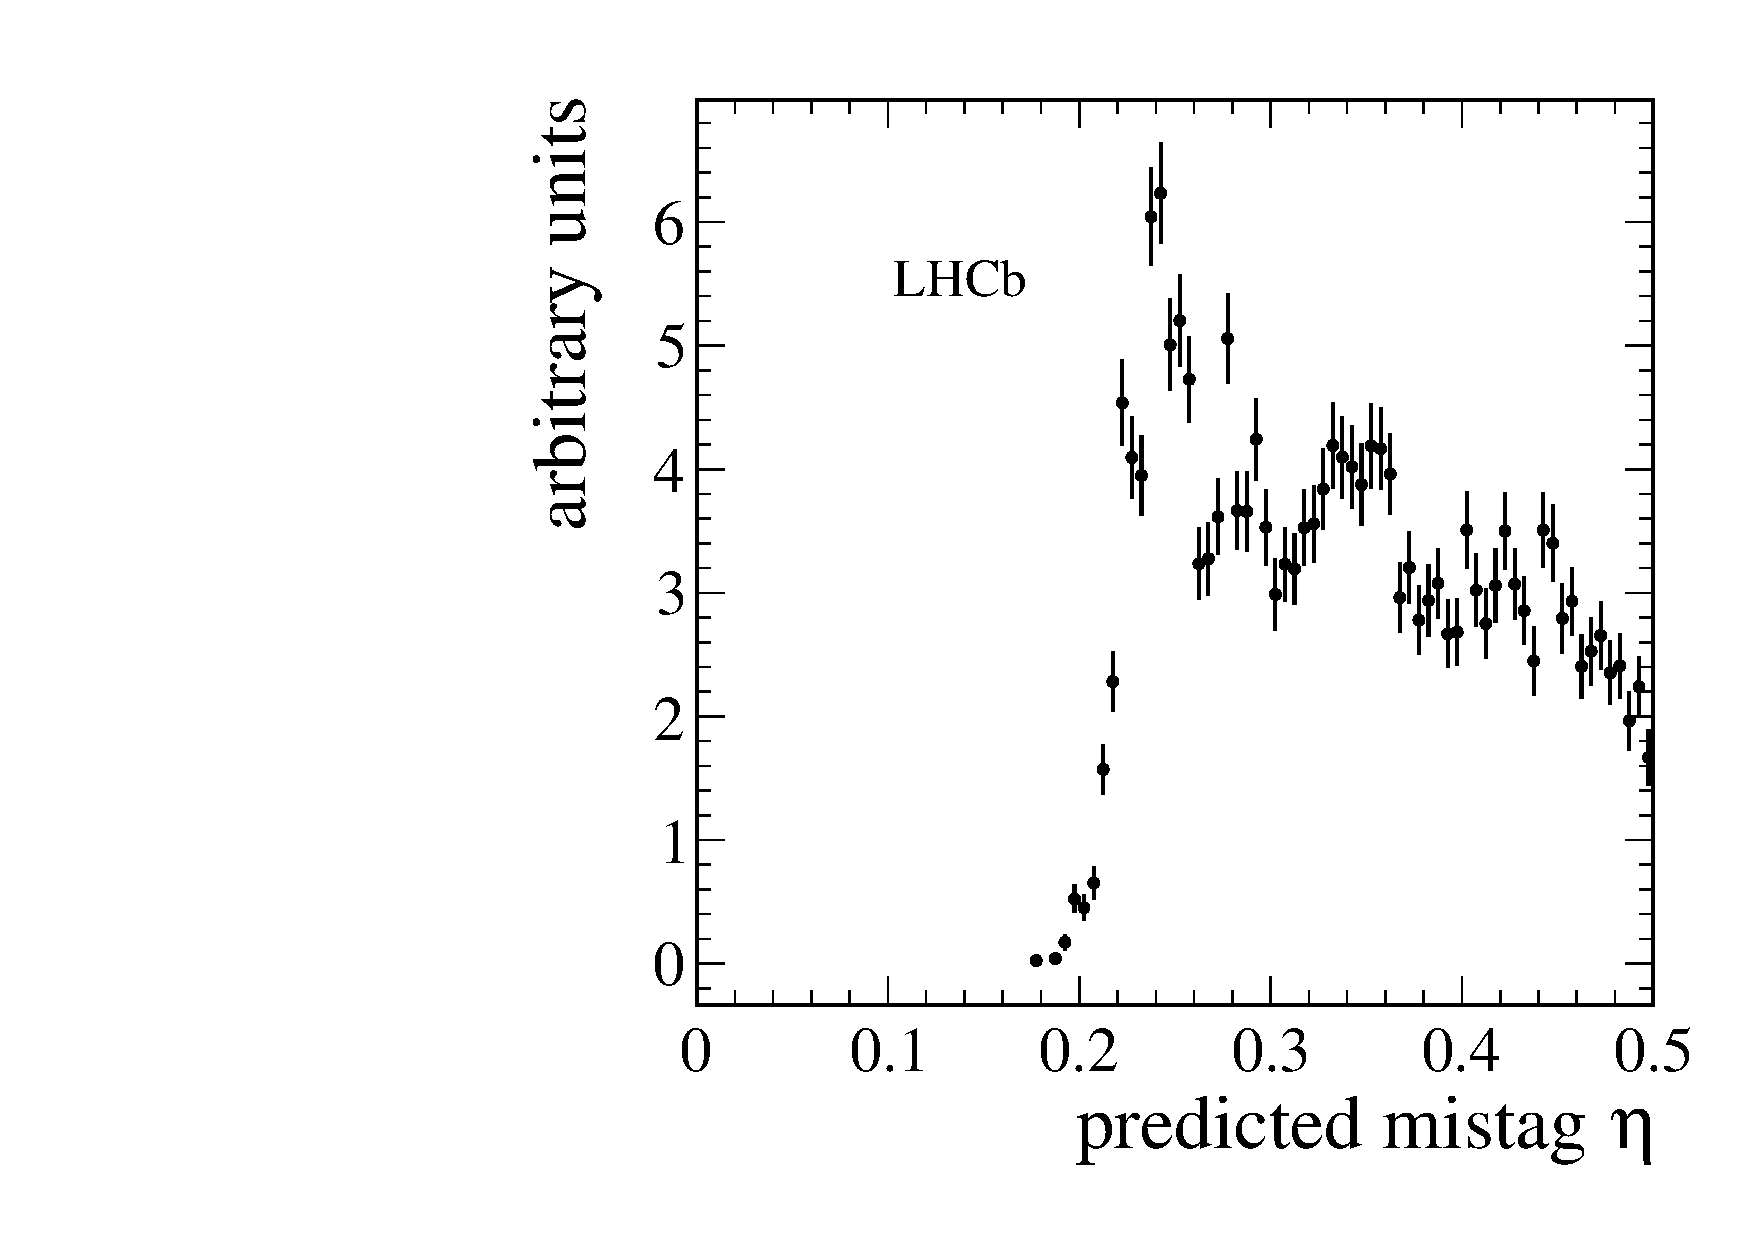
\includegraphics[width=0.26\textwidth]{04FlavourTagging/figs/OSelectronOpt/run1data_new/OS_Electron_EtaDist.pdf}
        \vspace{-2mm}
        \caption{Top: mistag calibration results on \emph{sWeighted} Run 1 $B^0\to D^-\pi^+$ data for the Run 1 old (left) and Run 1 new (right) versions of the \OSe~tagger. The \emph{sWeighted} data sample is shown as black points. The green (yellow) band indicates the 68\% (95\%) C.L. interval for the fitted calibration functions. Bottom: distributions of the uncalibrated mistag $\eta$.}
        \label{fig:OSePerfCalib1}
\end{figure}

\begin{figure}[hb!]
  \centering
  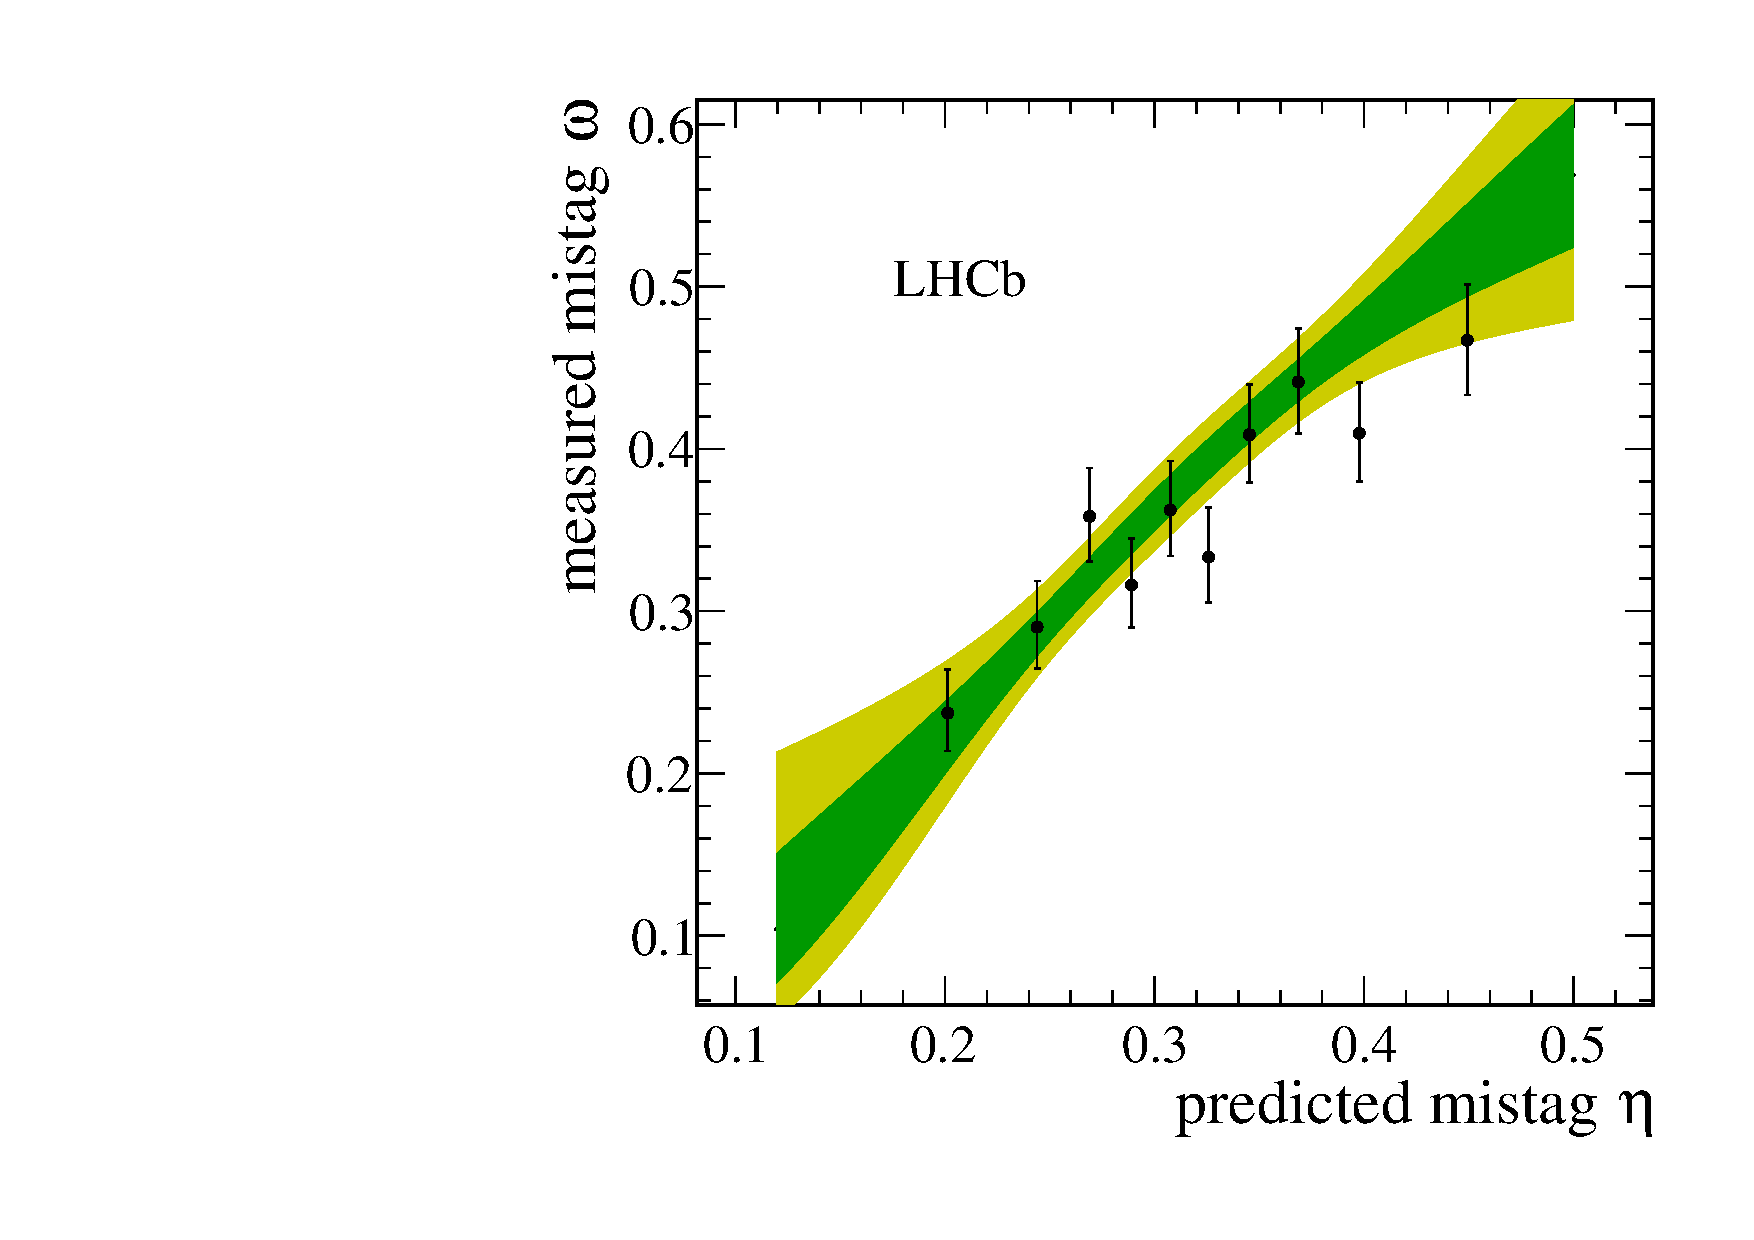
\includegraphics[width=0.26\textwidth]{04FlavourTagging/figs/OSelectronOpt/run1_tunings/OS_Electron_InputCalibration.pdf}
  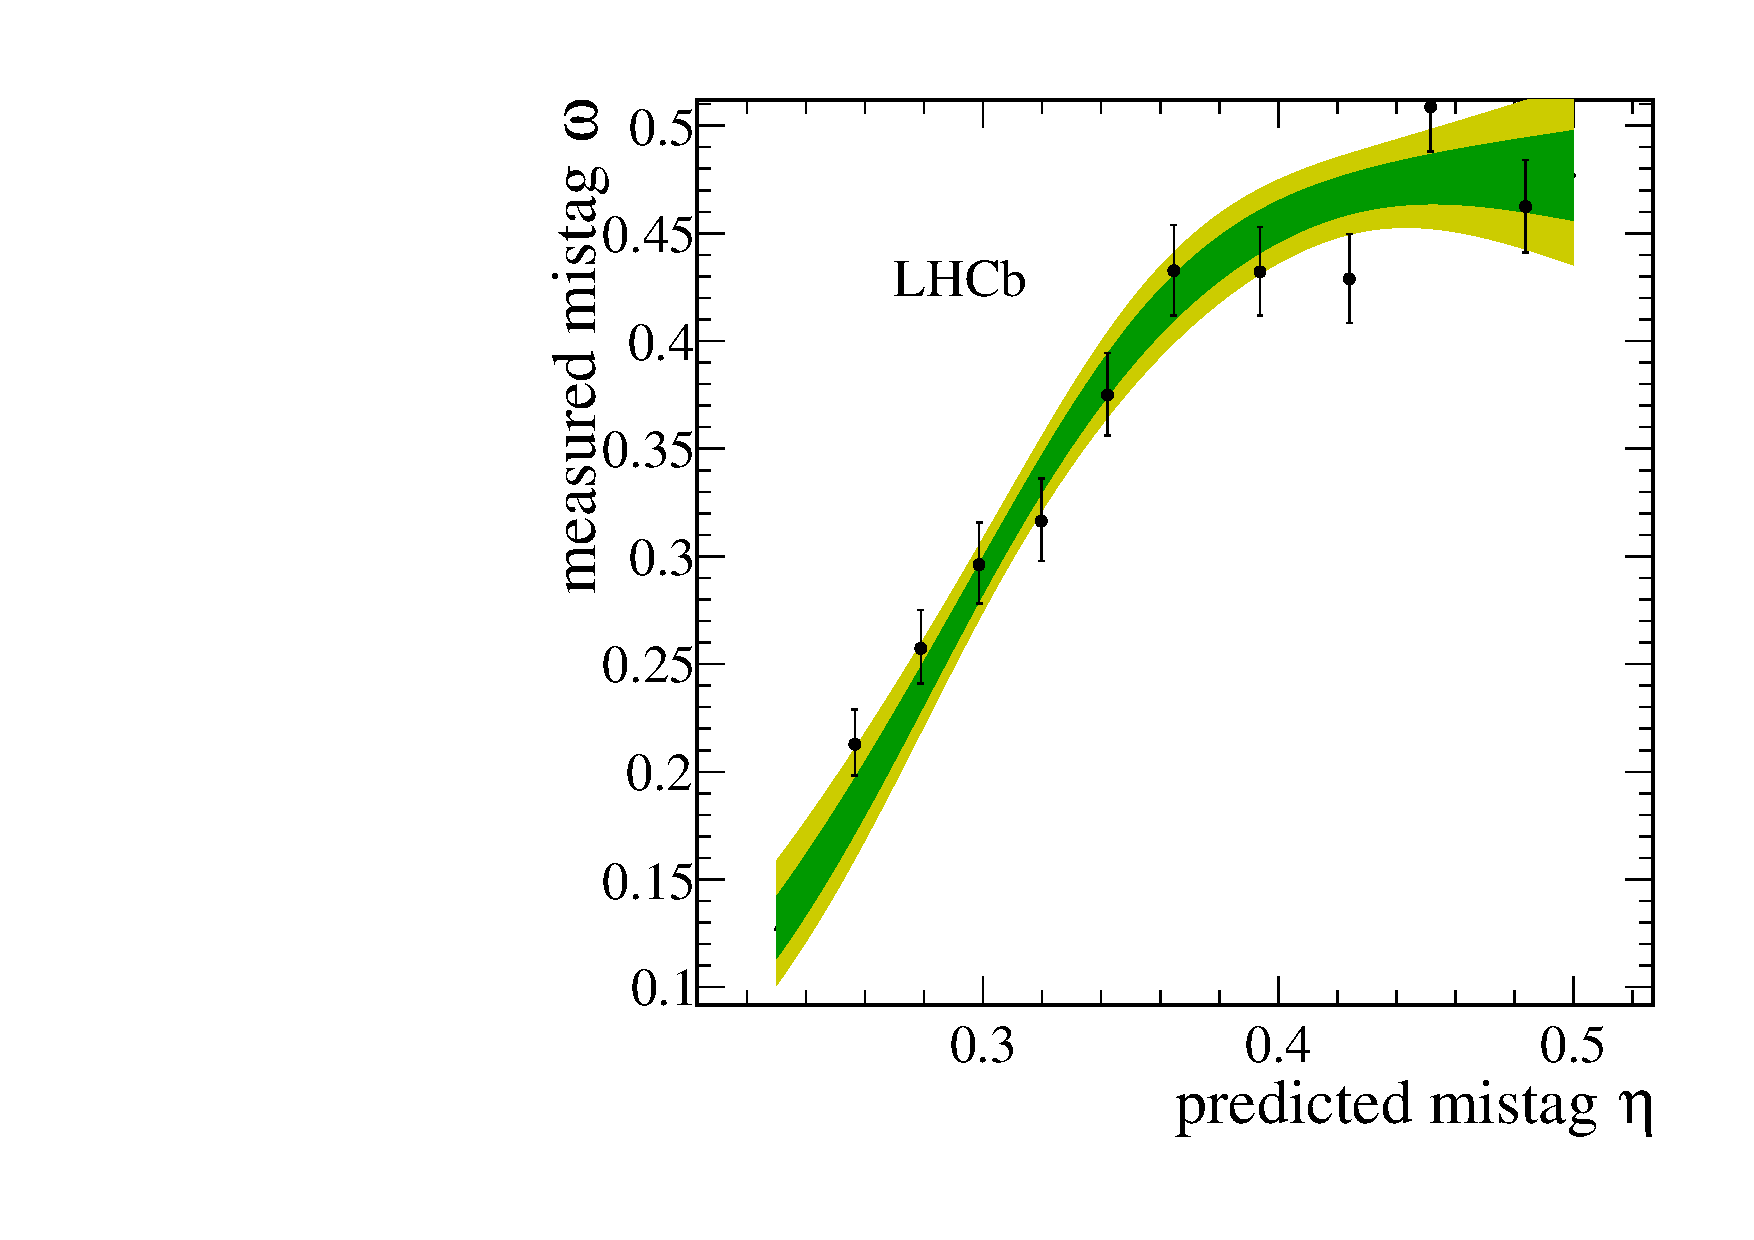
\includegraphics[width=0.26\textwidth]{04FlavourTagging/figs/OSelectronOpt/run2b2cc_tunings/OS_Electron_InputCalibration.pdf}
  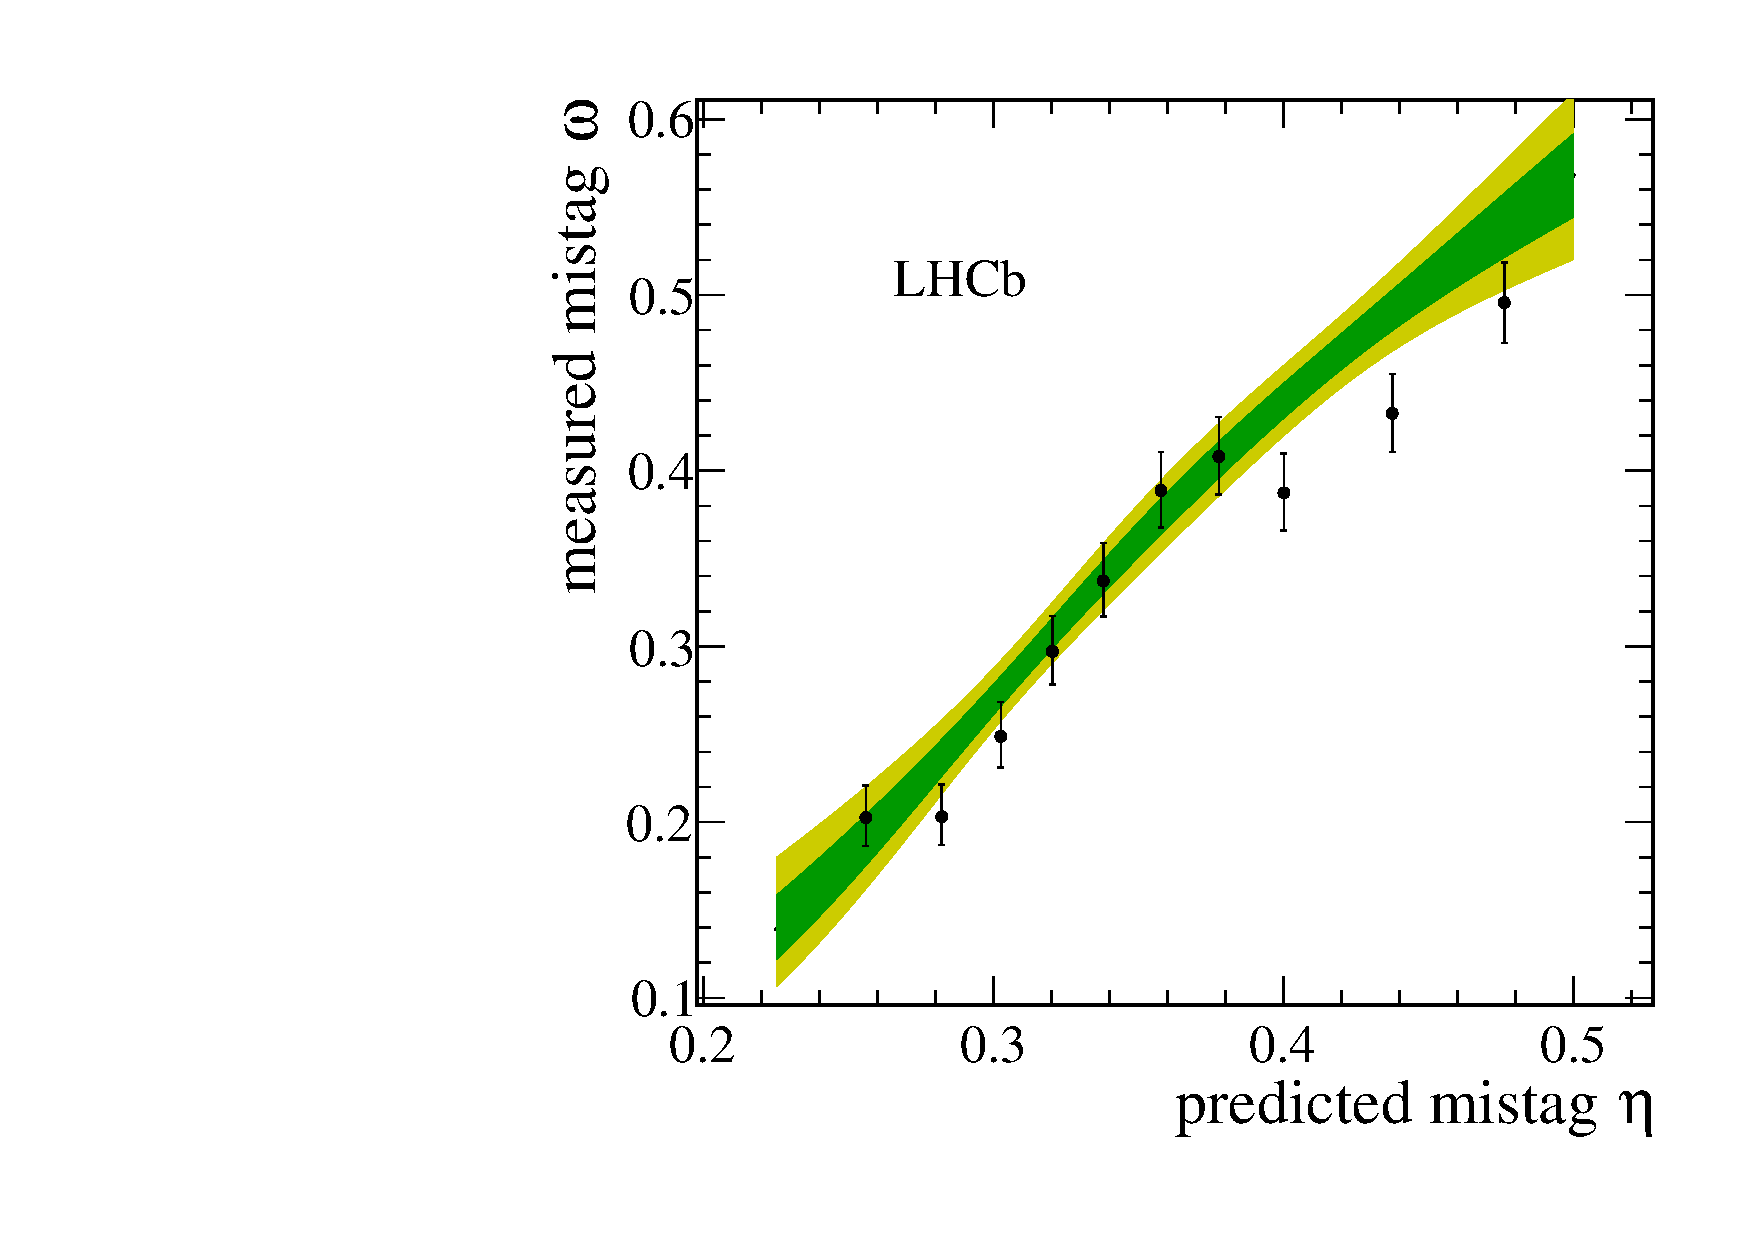
\includegraphics[width=0.26\textwidth]{04FlavourTagging/figs/OSelectronOpt/run2b2oc_tunings/OS_Electron_InputCalibration.pdf} \\
  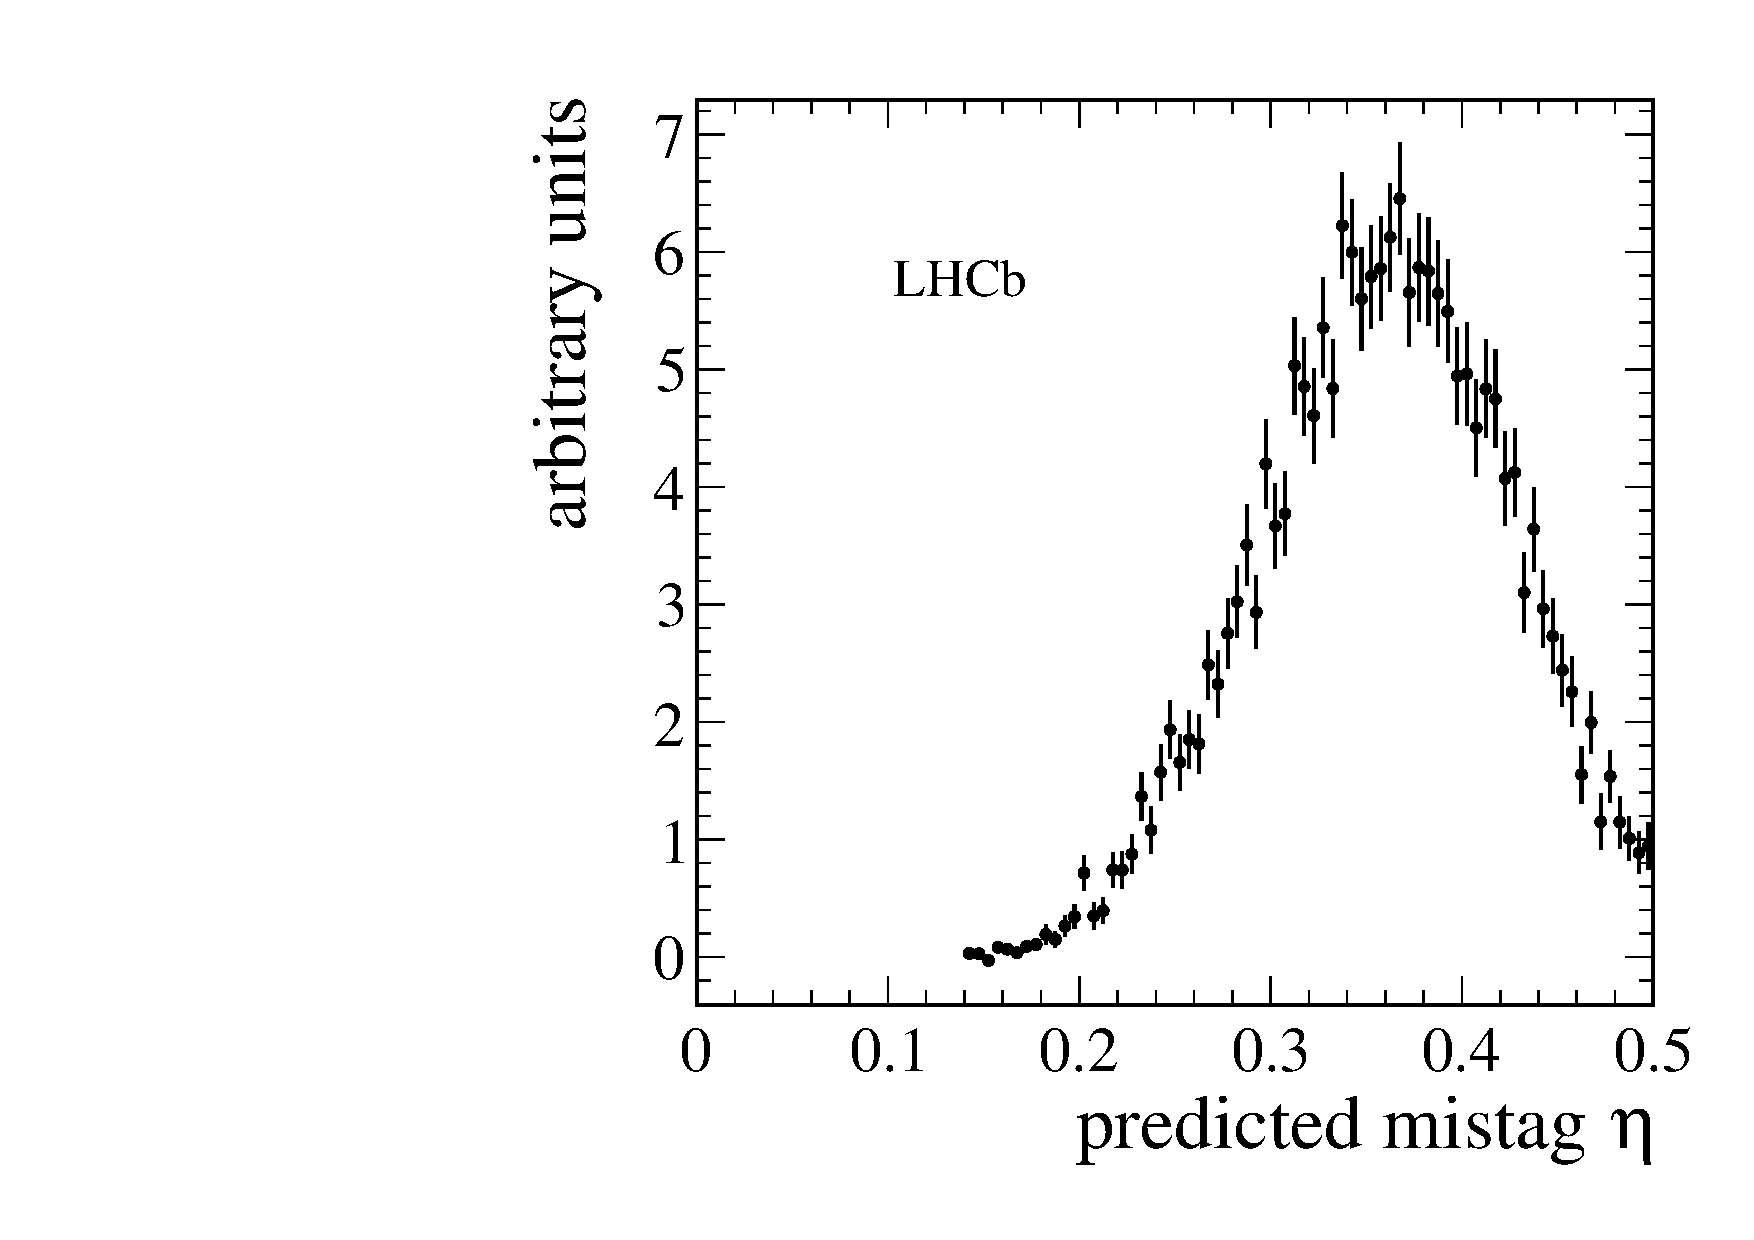
\includegraphics[width=0.26\textwidth]{04FlavourTagging/figs/OSelectronOpt/run1_tunings/OS_Electron_EtaDist.pdf}
  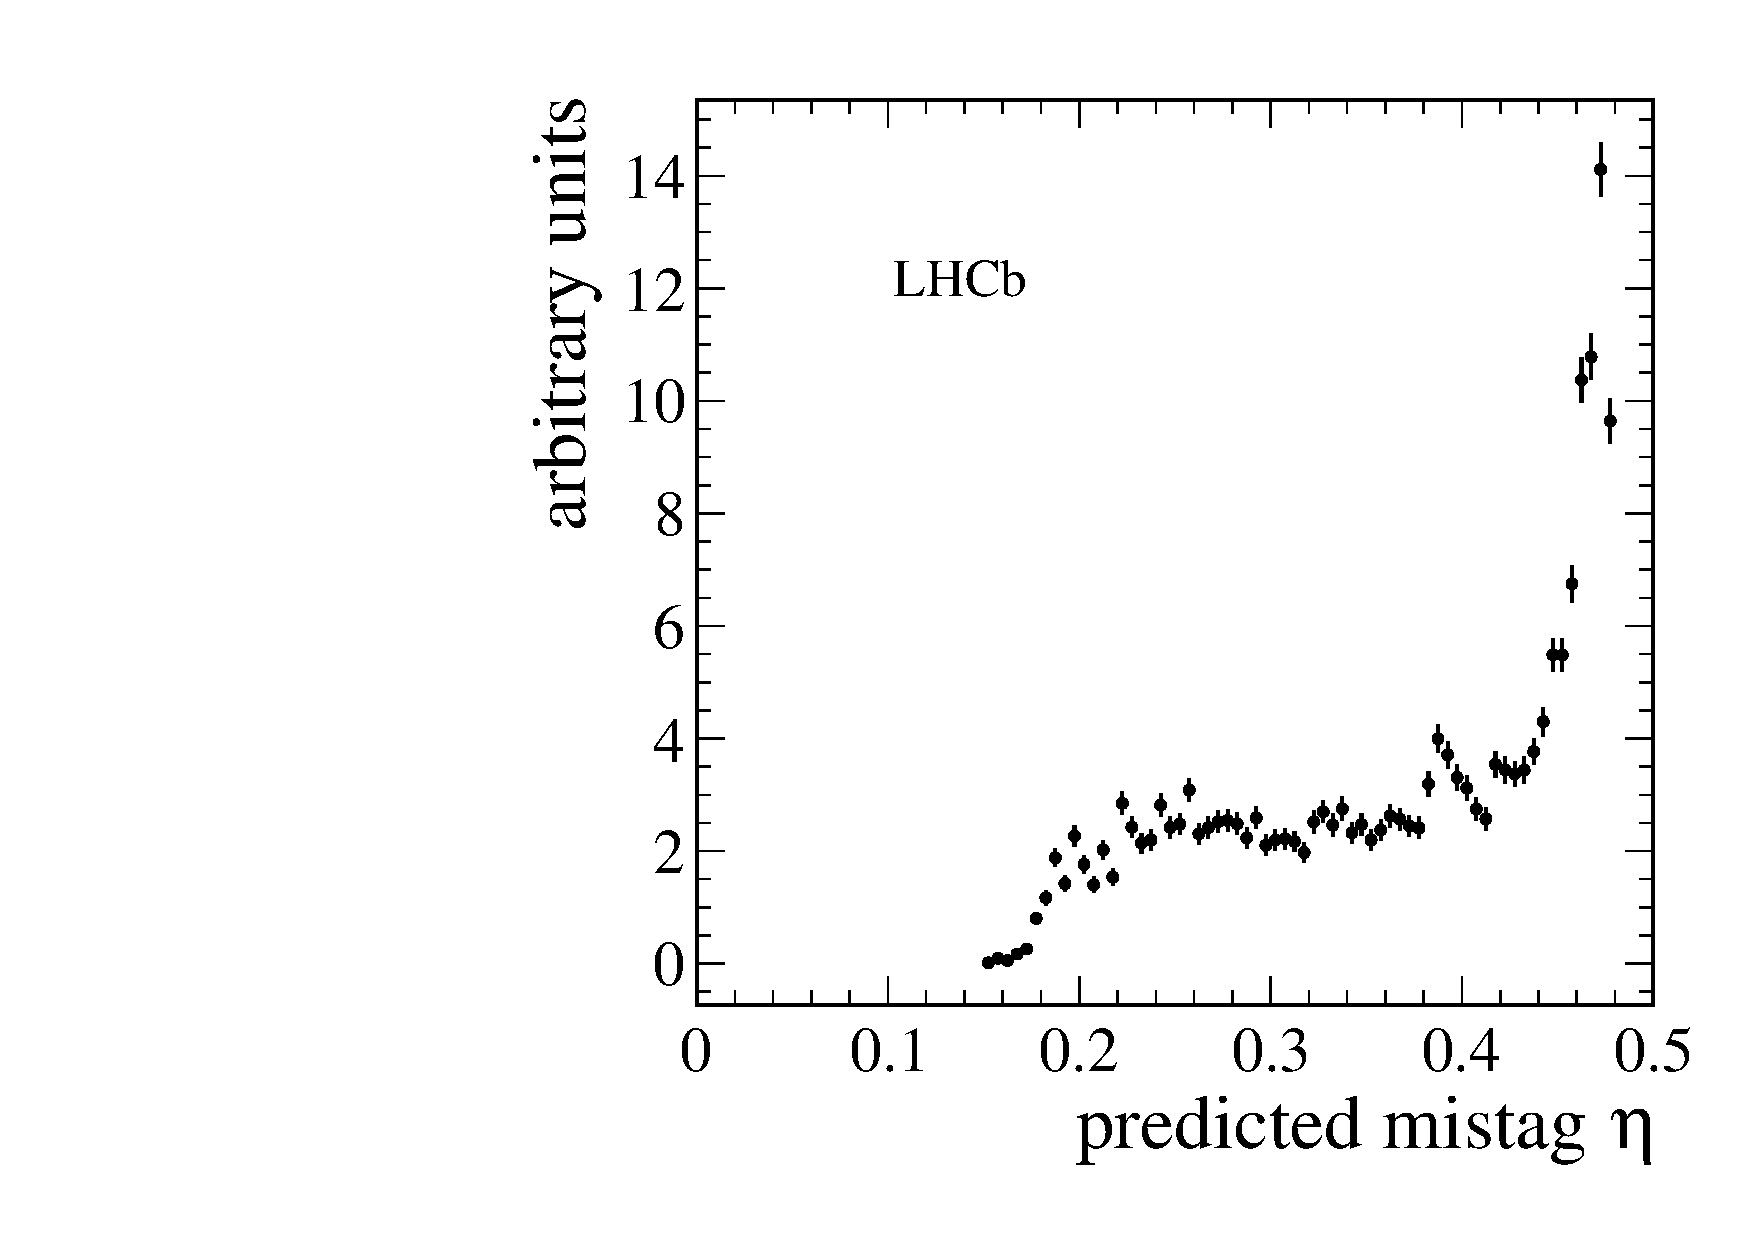
\includegraphics[width=0.26\textwidth]{04FlavourTagging/figs/OSelectronOpt/run2b2cc_tunings/OS_Electron_EtaDist.pdf}
  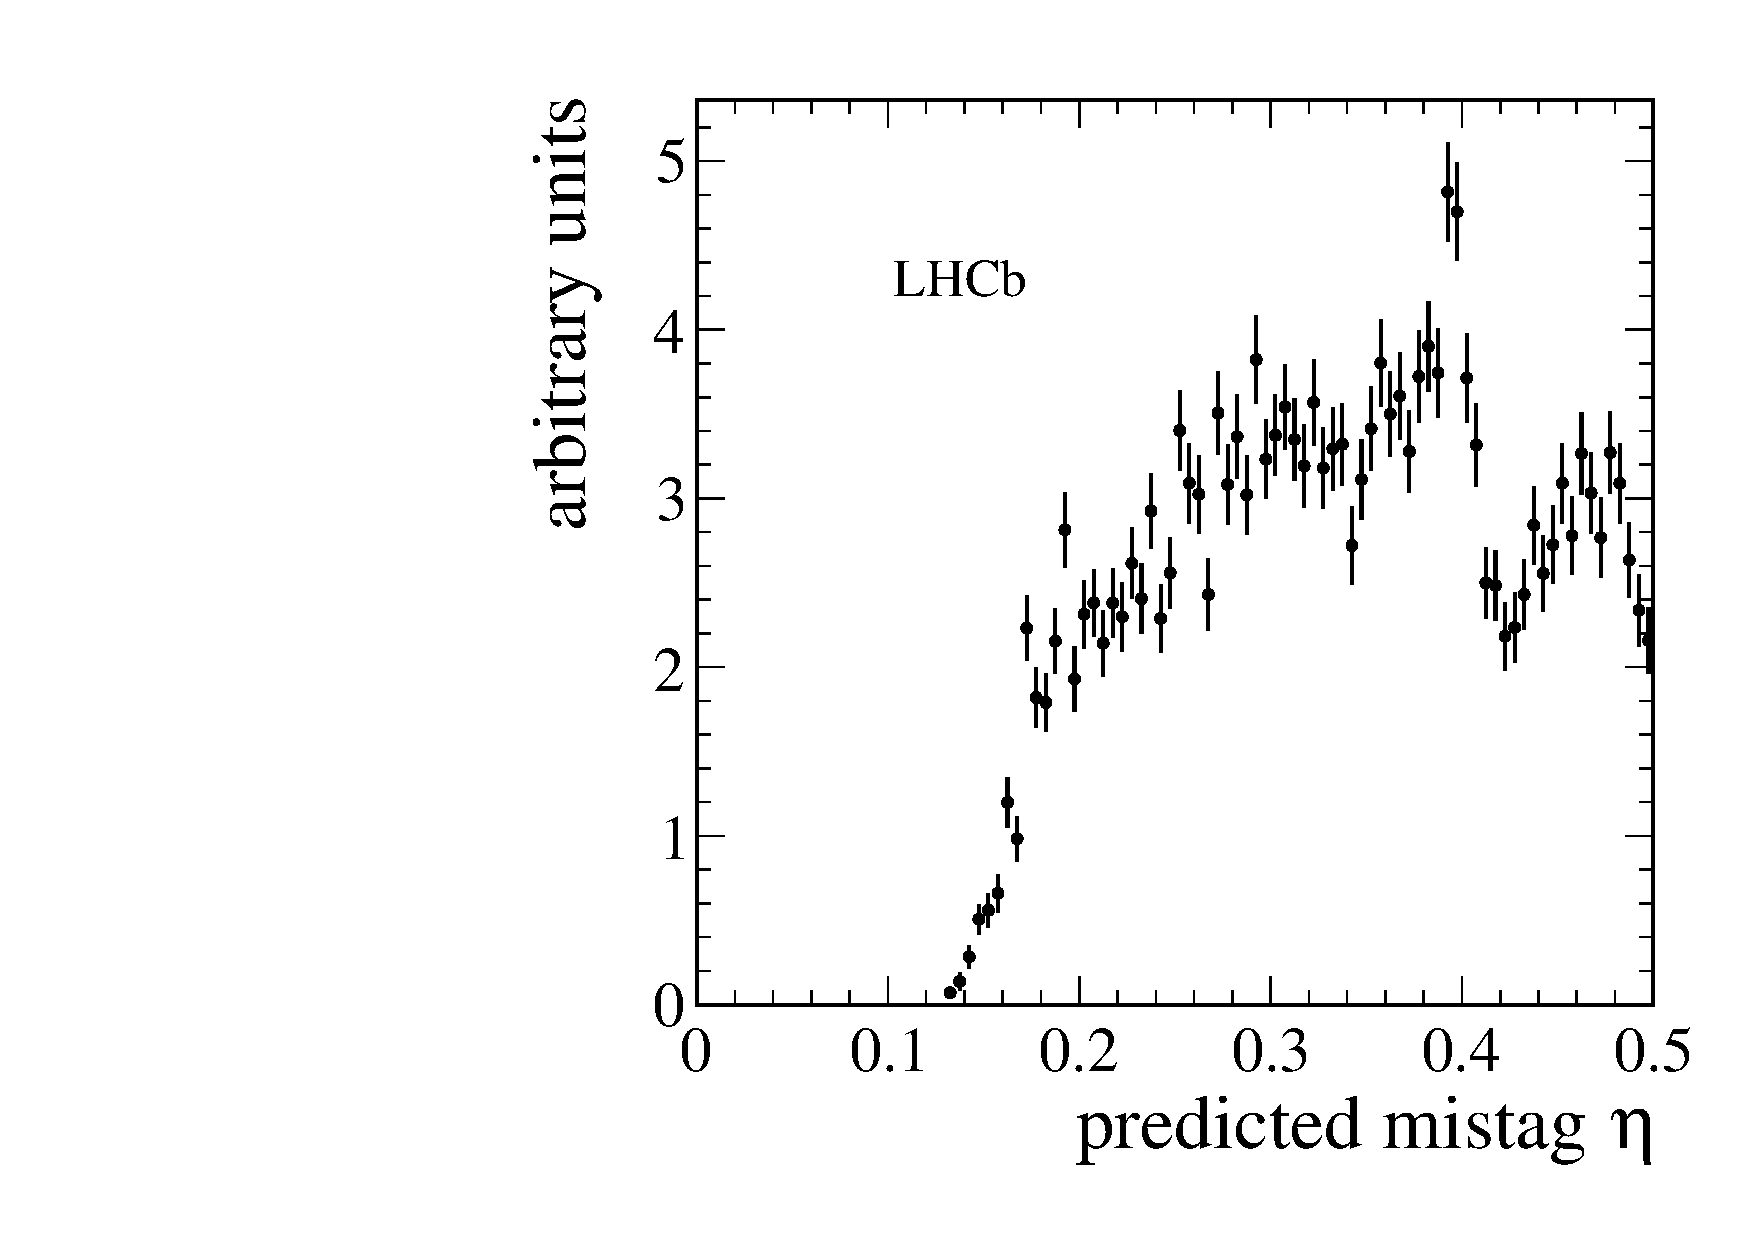
\includegraphics[width=0.26\textwidth]{04FlavourTagging/figs/OSelectronOpt/run2b2oc_tunings/OS_Electron_EtaDist.pdf}
  \caption{Mistag calibration results on \emph{sWeighted} Run 2 $B^0\to D^-\pi^+$ data for the \OSe~taggers. The results obtained with the Run 1 old (left), Run 2 B2CC (center), and Run 2 B2OC (right) tunings are shown.
The \emph{sWeighted} data sample is shown as black points. The green (yellow) band indicates the 68\% (95\%) C.L. interval for the fitted calibration functions. Bottom: distributions of the uncalibrated mistag $\eta$.}
  \label{fig:OSePerfCalib3}
\end{figure}


\begin{figure}[ht!]
  \centering
  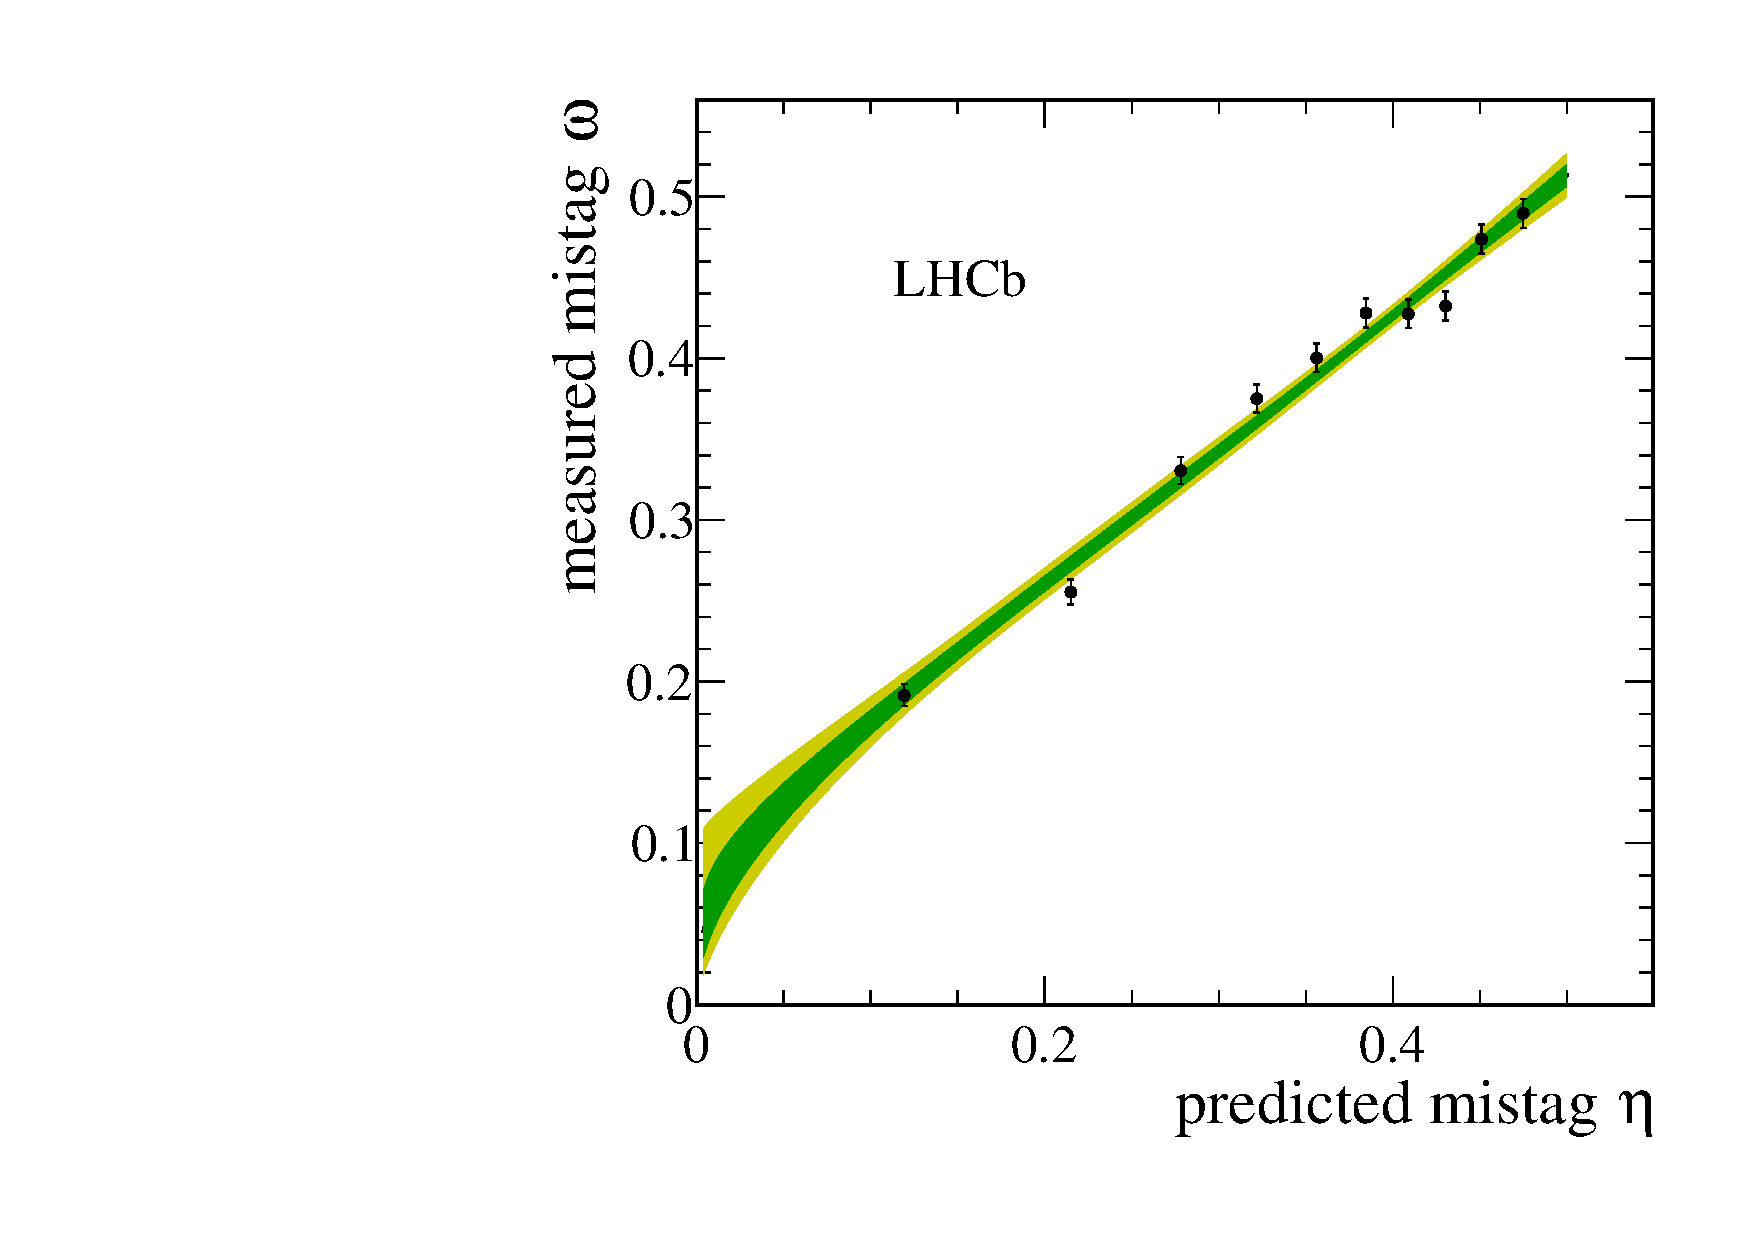
\includegraphics[width=0.26\textwidth]{04FlavourTagging/figs/OSelectronOpt/run1data_old/OS_Combination_Calibration.pdf}
  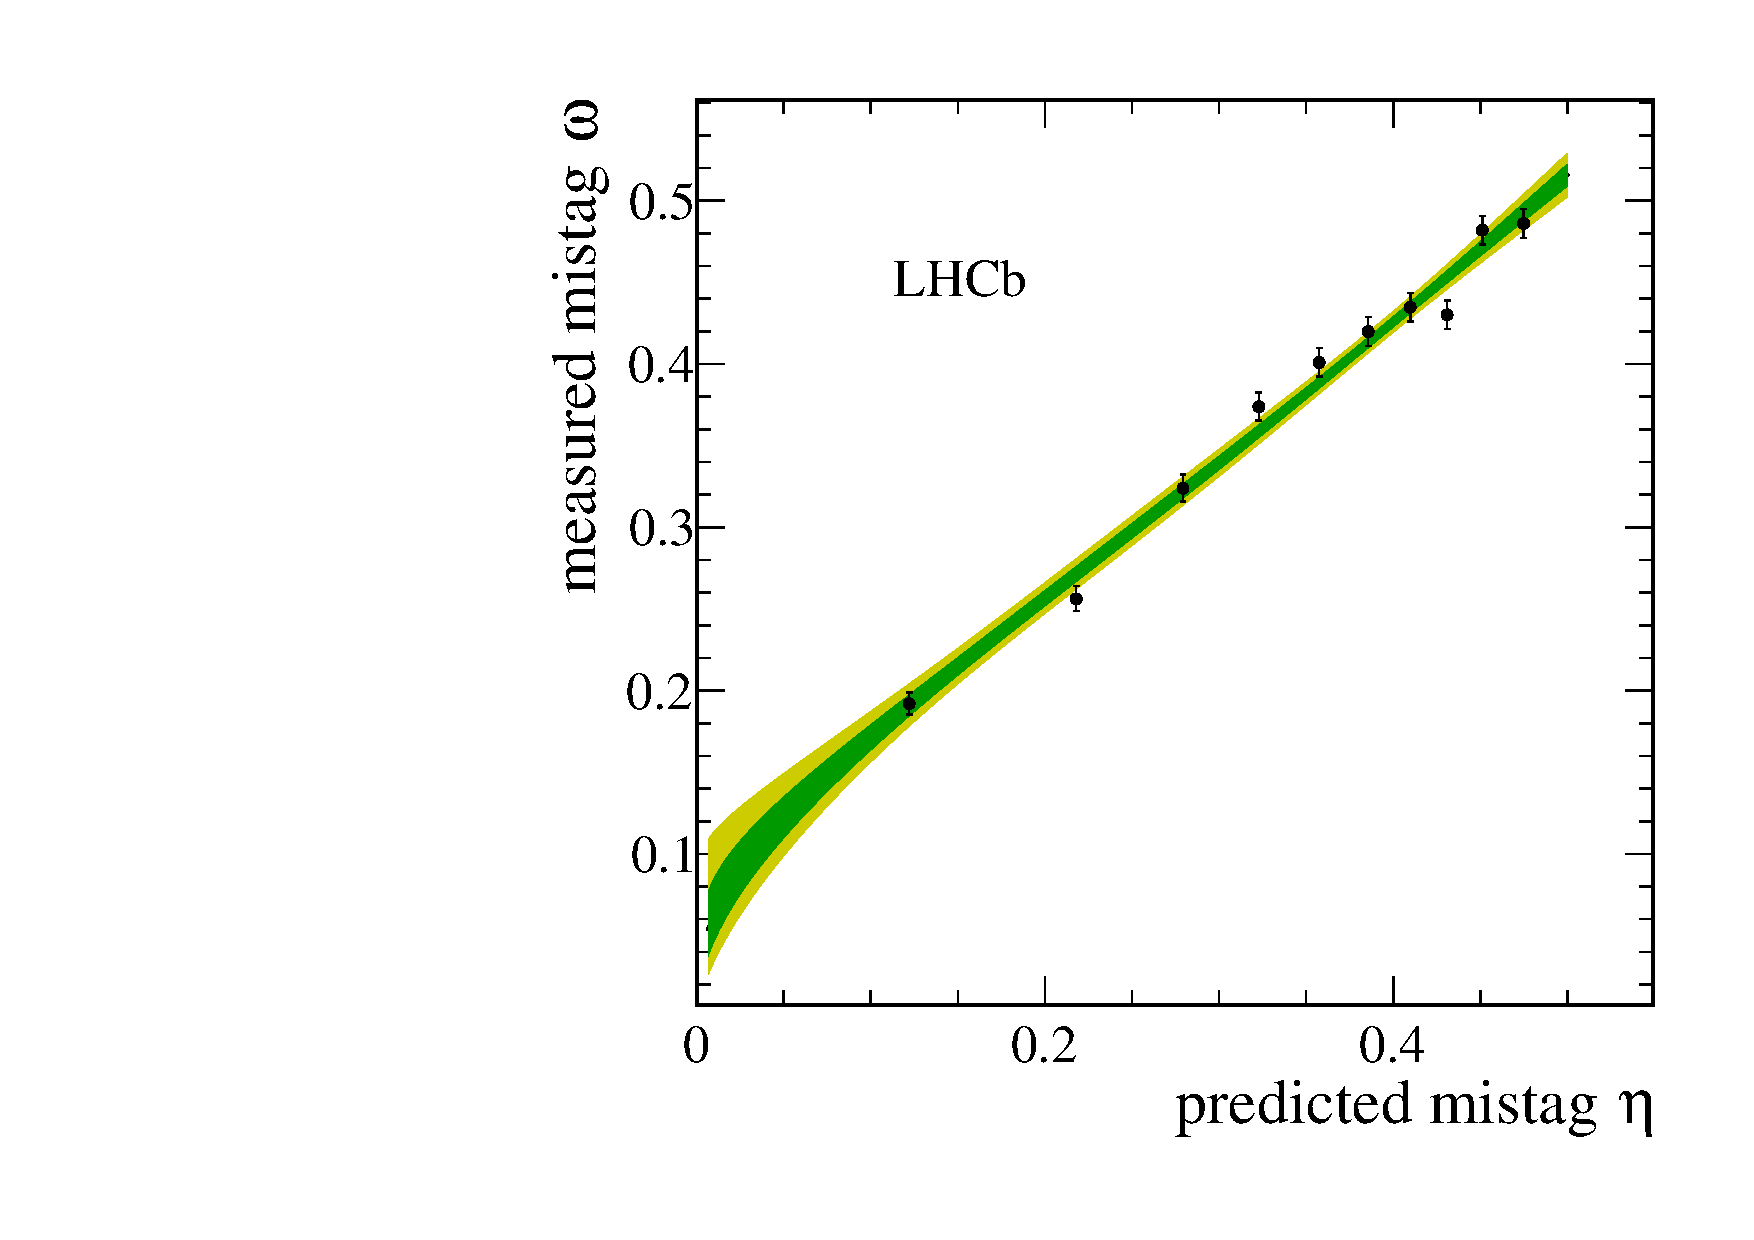
\includegraphics[width=0.26\textwidth]{04FlavourTagging/figs/OSelectronOpt/run1data_new/OS_Combination_Calibration.pdf} \\
  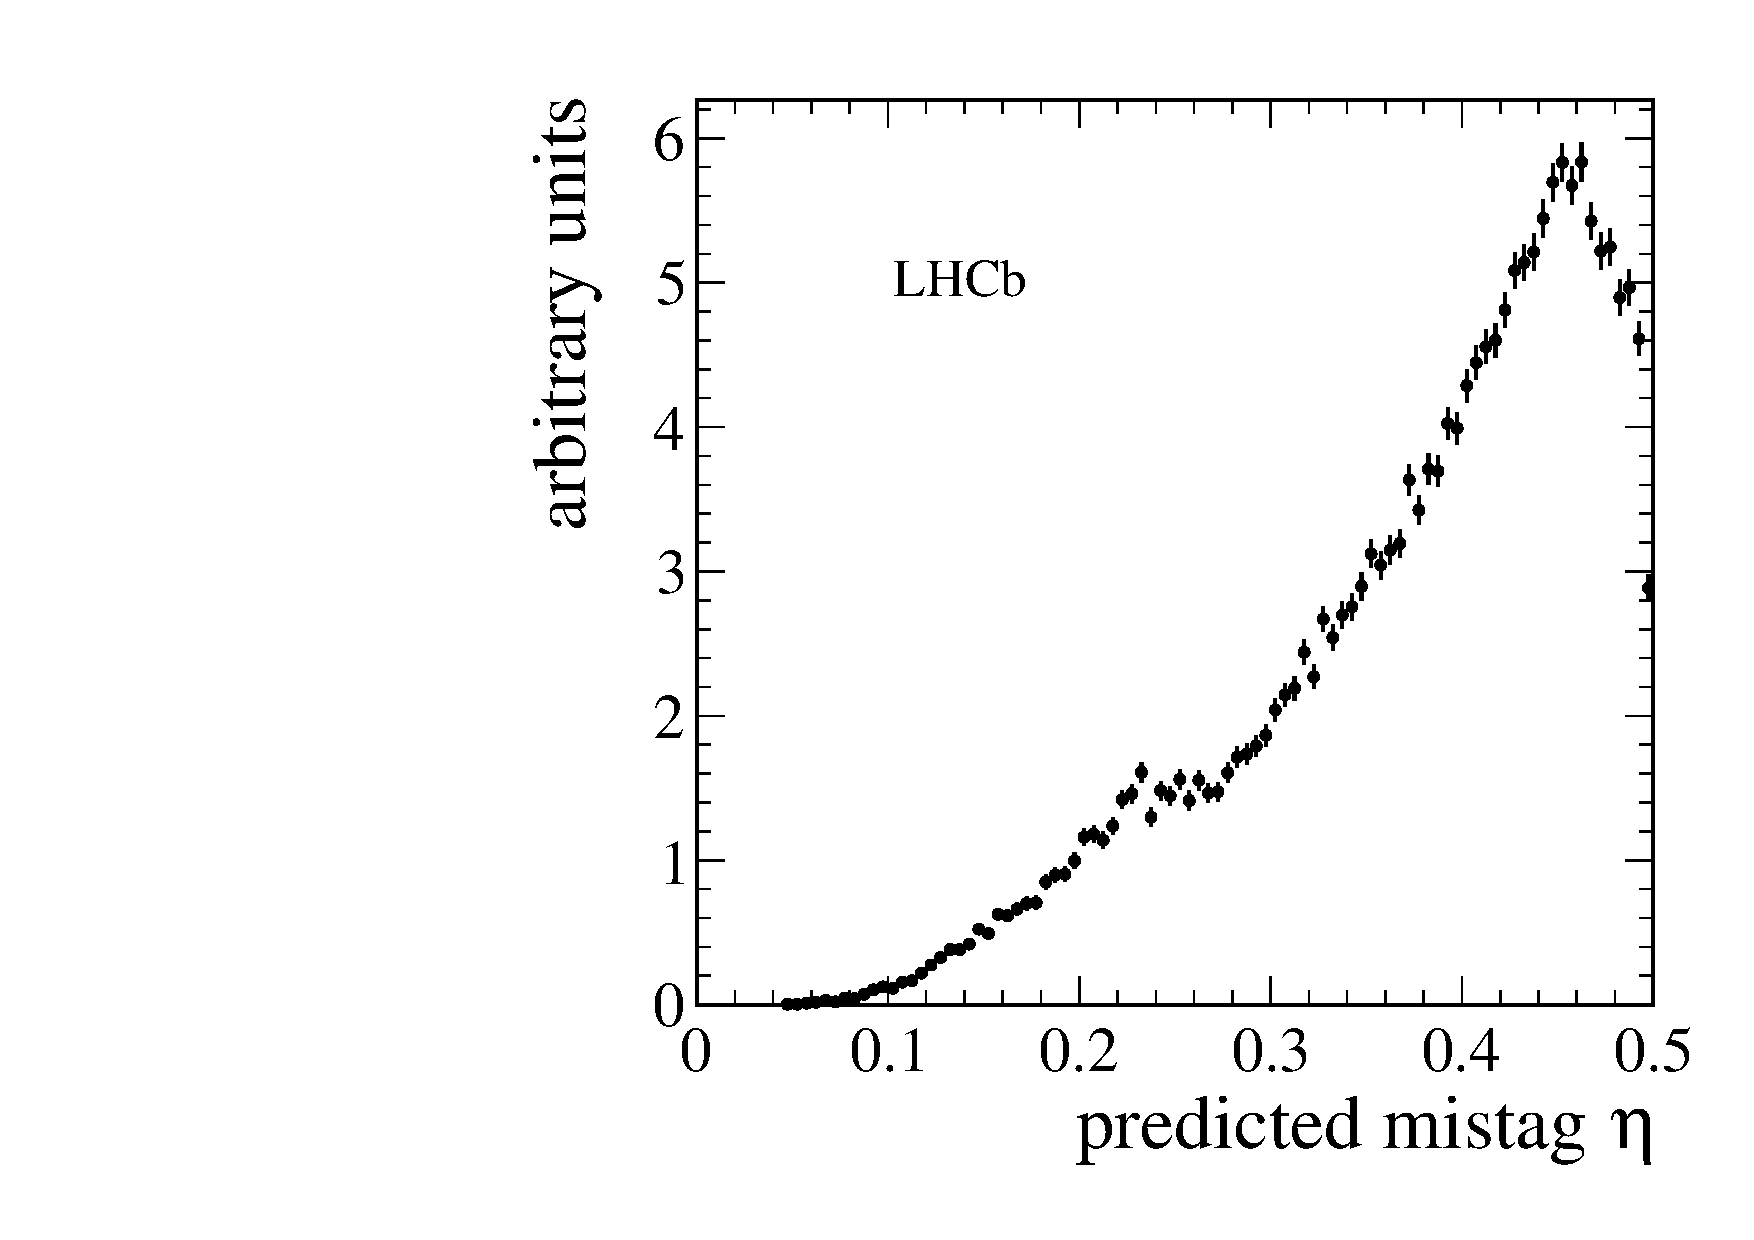
\includegraphics[width=0.26\textwidth]{04FlavourTagging/figs/OSelectronOpt/run1data_old/OS_Combination_EtaDist.pdf}
  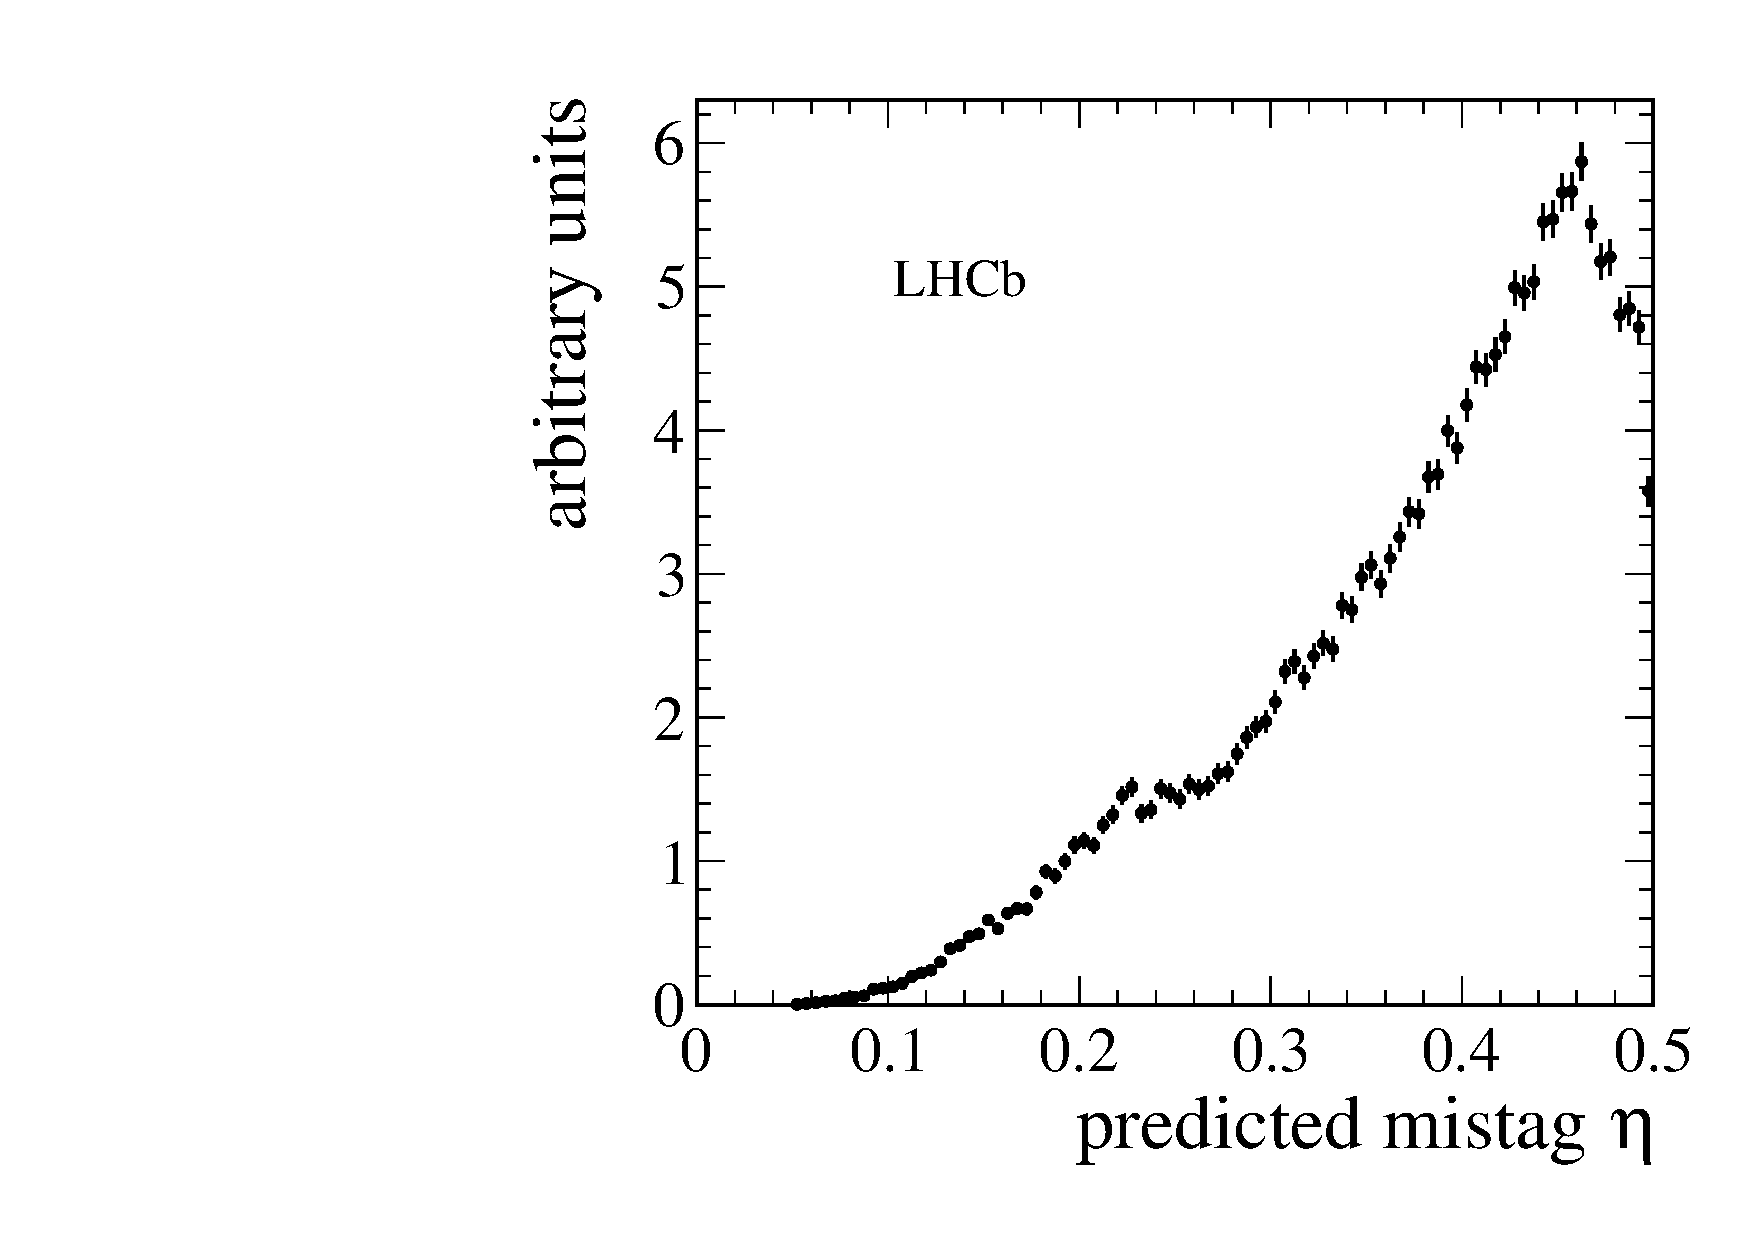
\includegraphics[width=0.26\textwidth]{04FlavourTagging/figs/OSelectronOpt/run1data_new/OS_Combination_EtaDist.pdf} 
  \vspace{-2mm}
  \caption{Top: mistag calibration results on \emph{sWeighted} Run 1 $B^0\to D^-\pi^+$ data for the combination of the OS taggers. The results obtained with the Run 1 old (left) and Run 1 new (right) tunings of \OSe~are shown. The \emph{sWeighted} data sample is shown as black points. The green (yellow) band indicates the 68\% (95\%) C.L. interval for the fitted calibration functions. Bottom: distributions of the uncalibrated mistag $\eta$.}
  \label{fig:OSePerfCalib2}
\end{figure}

\begin{figure}[hb!]
  \centering
  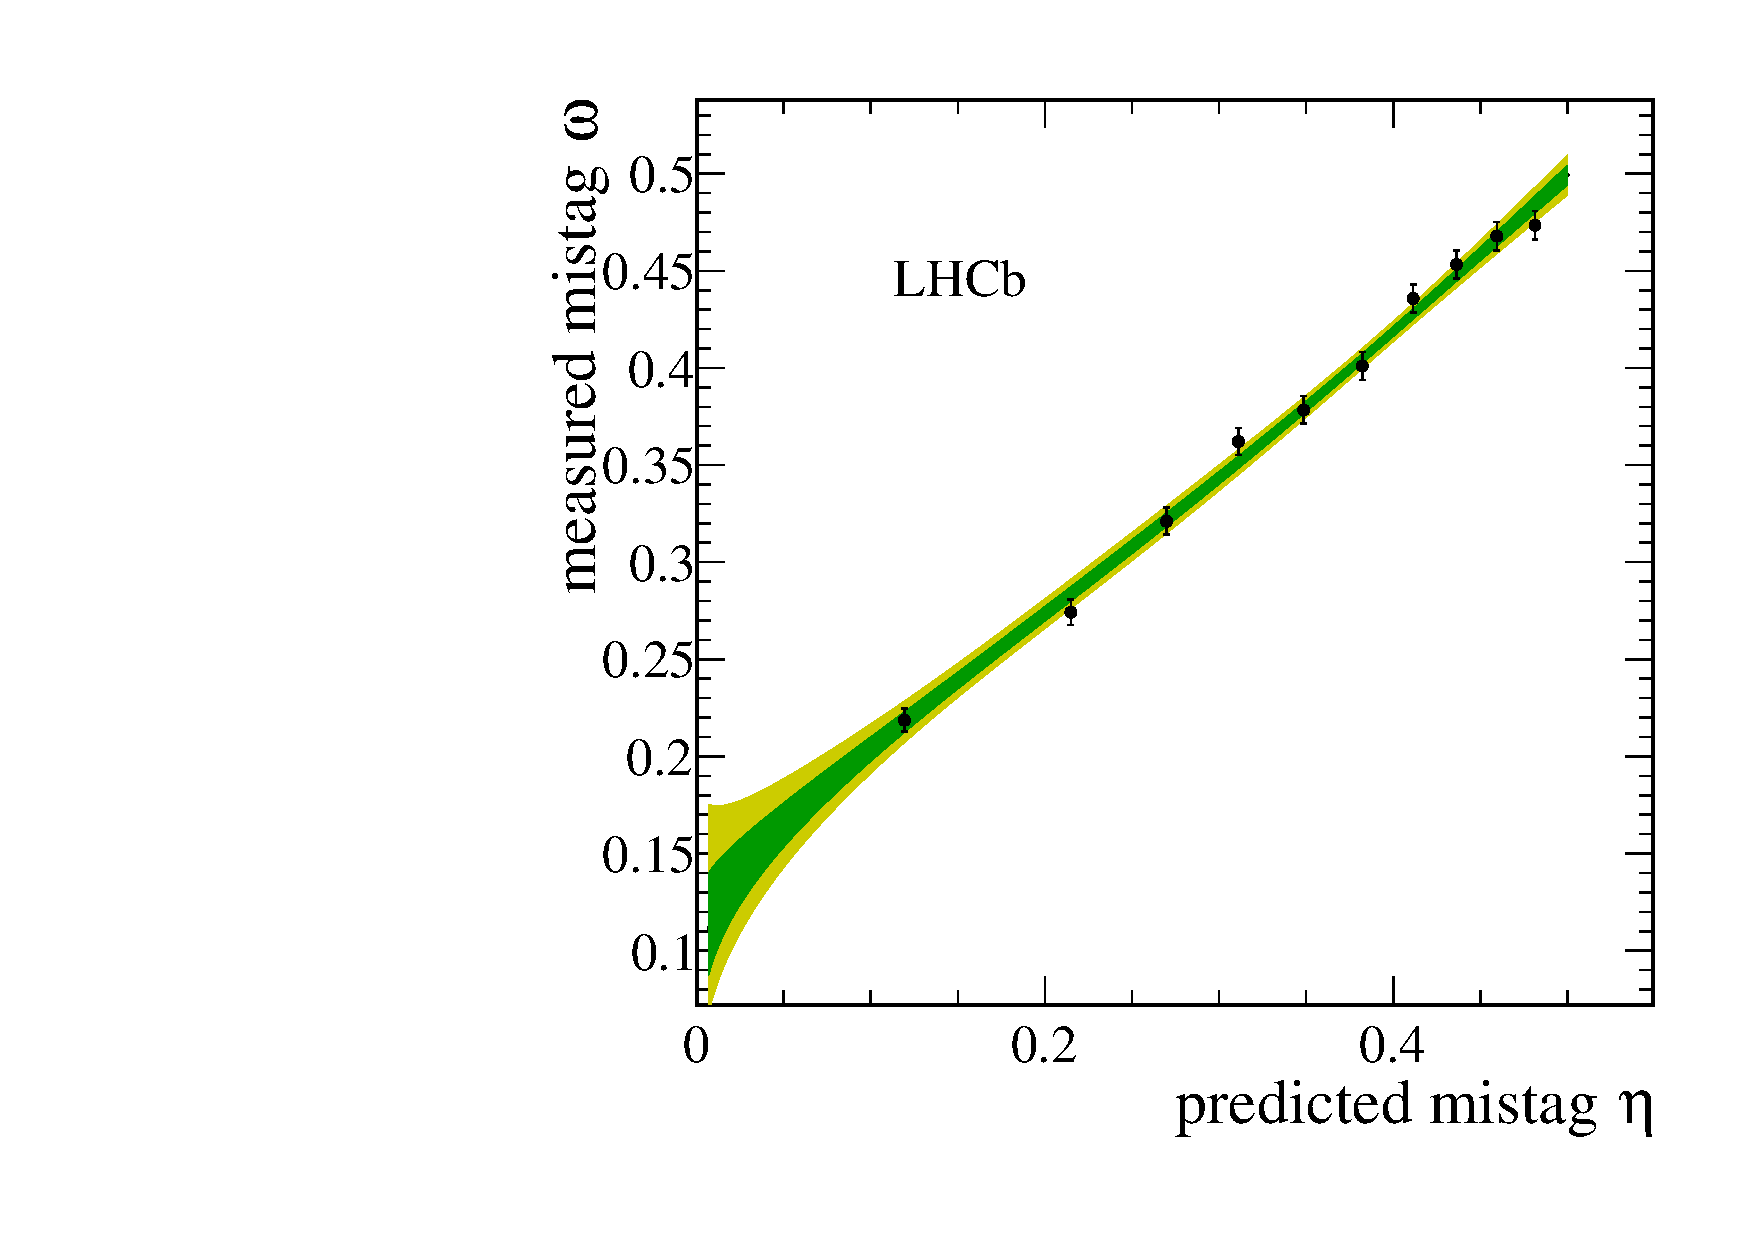
\includegraphics[width=0.26\textwidth]{04FlavourTagging/figs/OSelectronOpt/run1_tunings/OS_Combination_Calibration.pdf}
  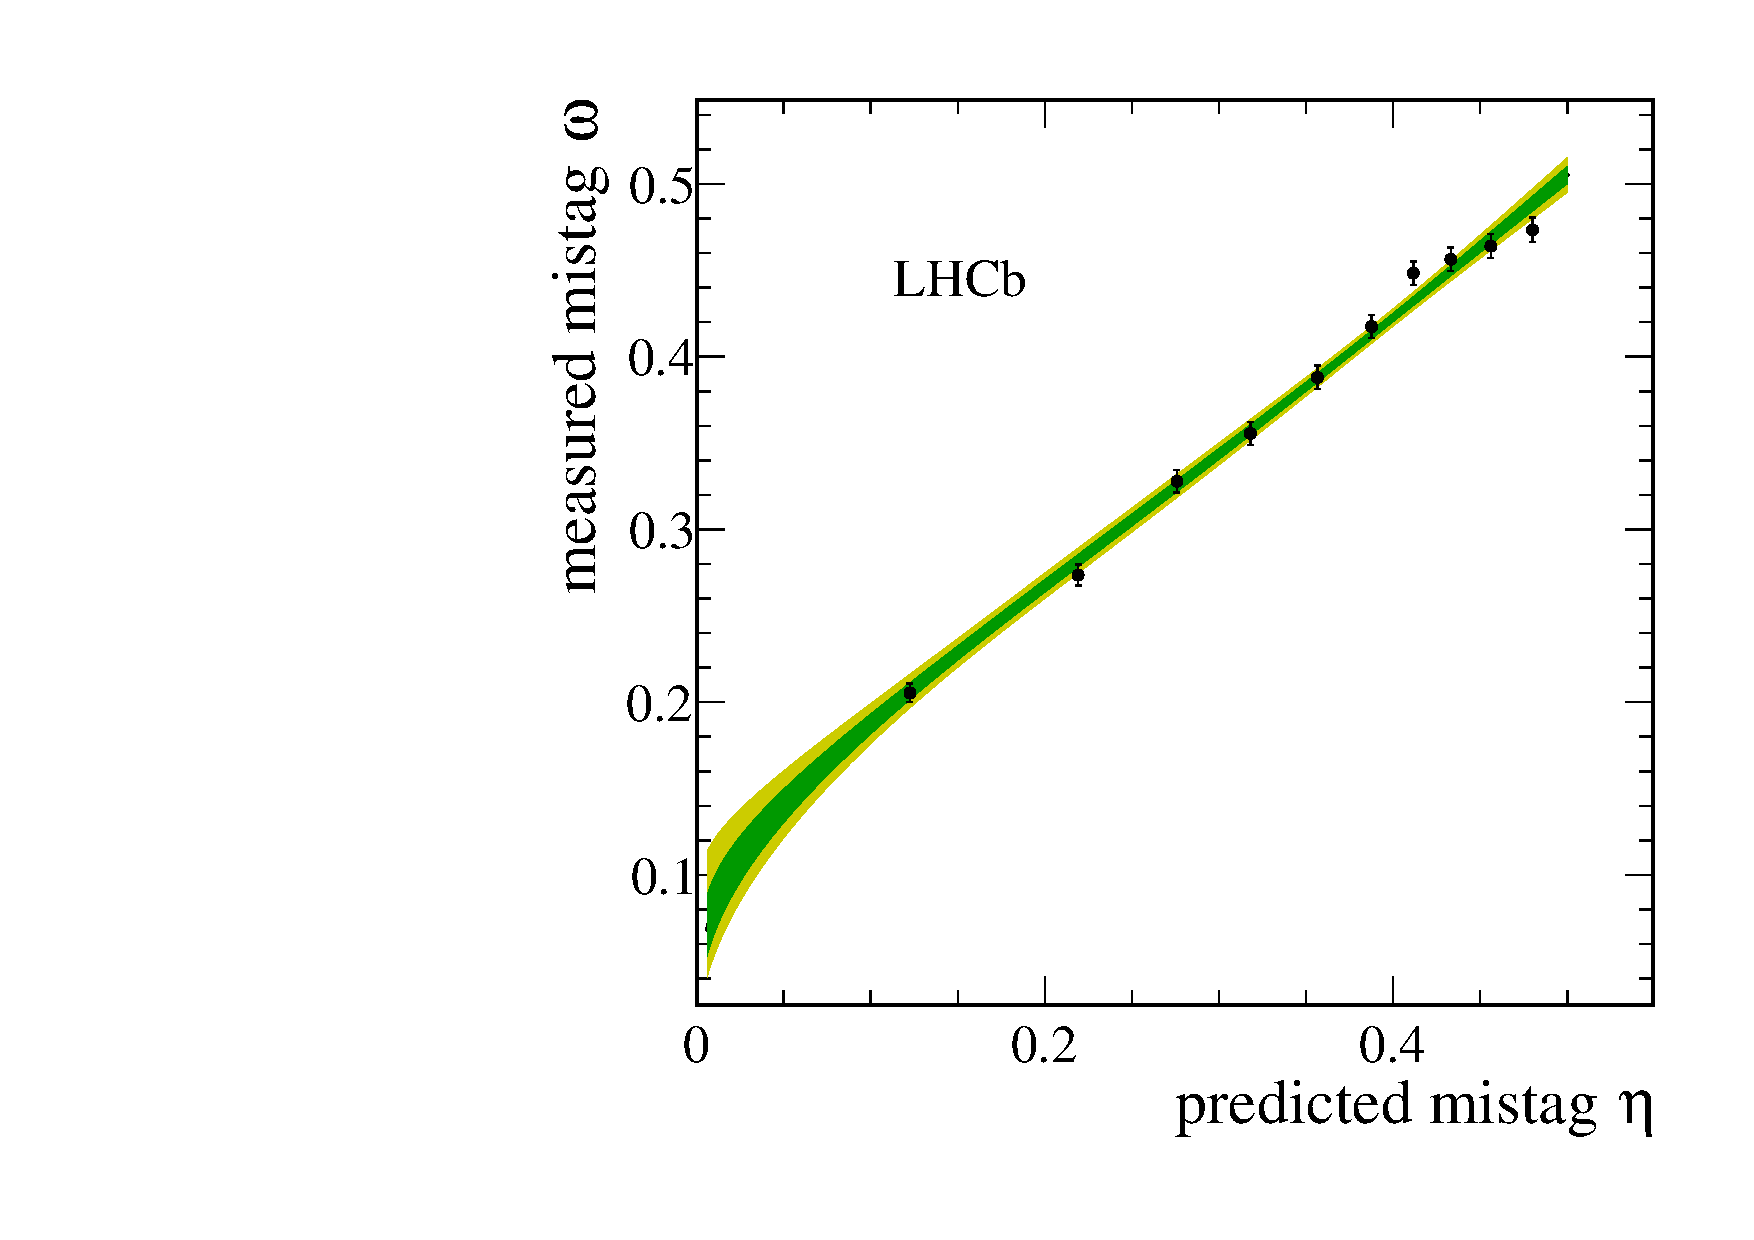
\includegraphics[width=0.26\textwidth]{04FlavourTagging/figs/OSelectronOpt/run2b2cc_tunings/OS_Combination_Calibration.pdf}
  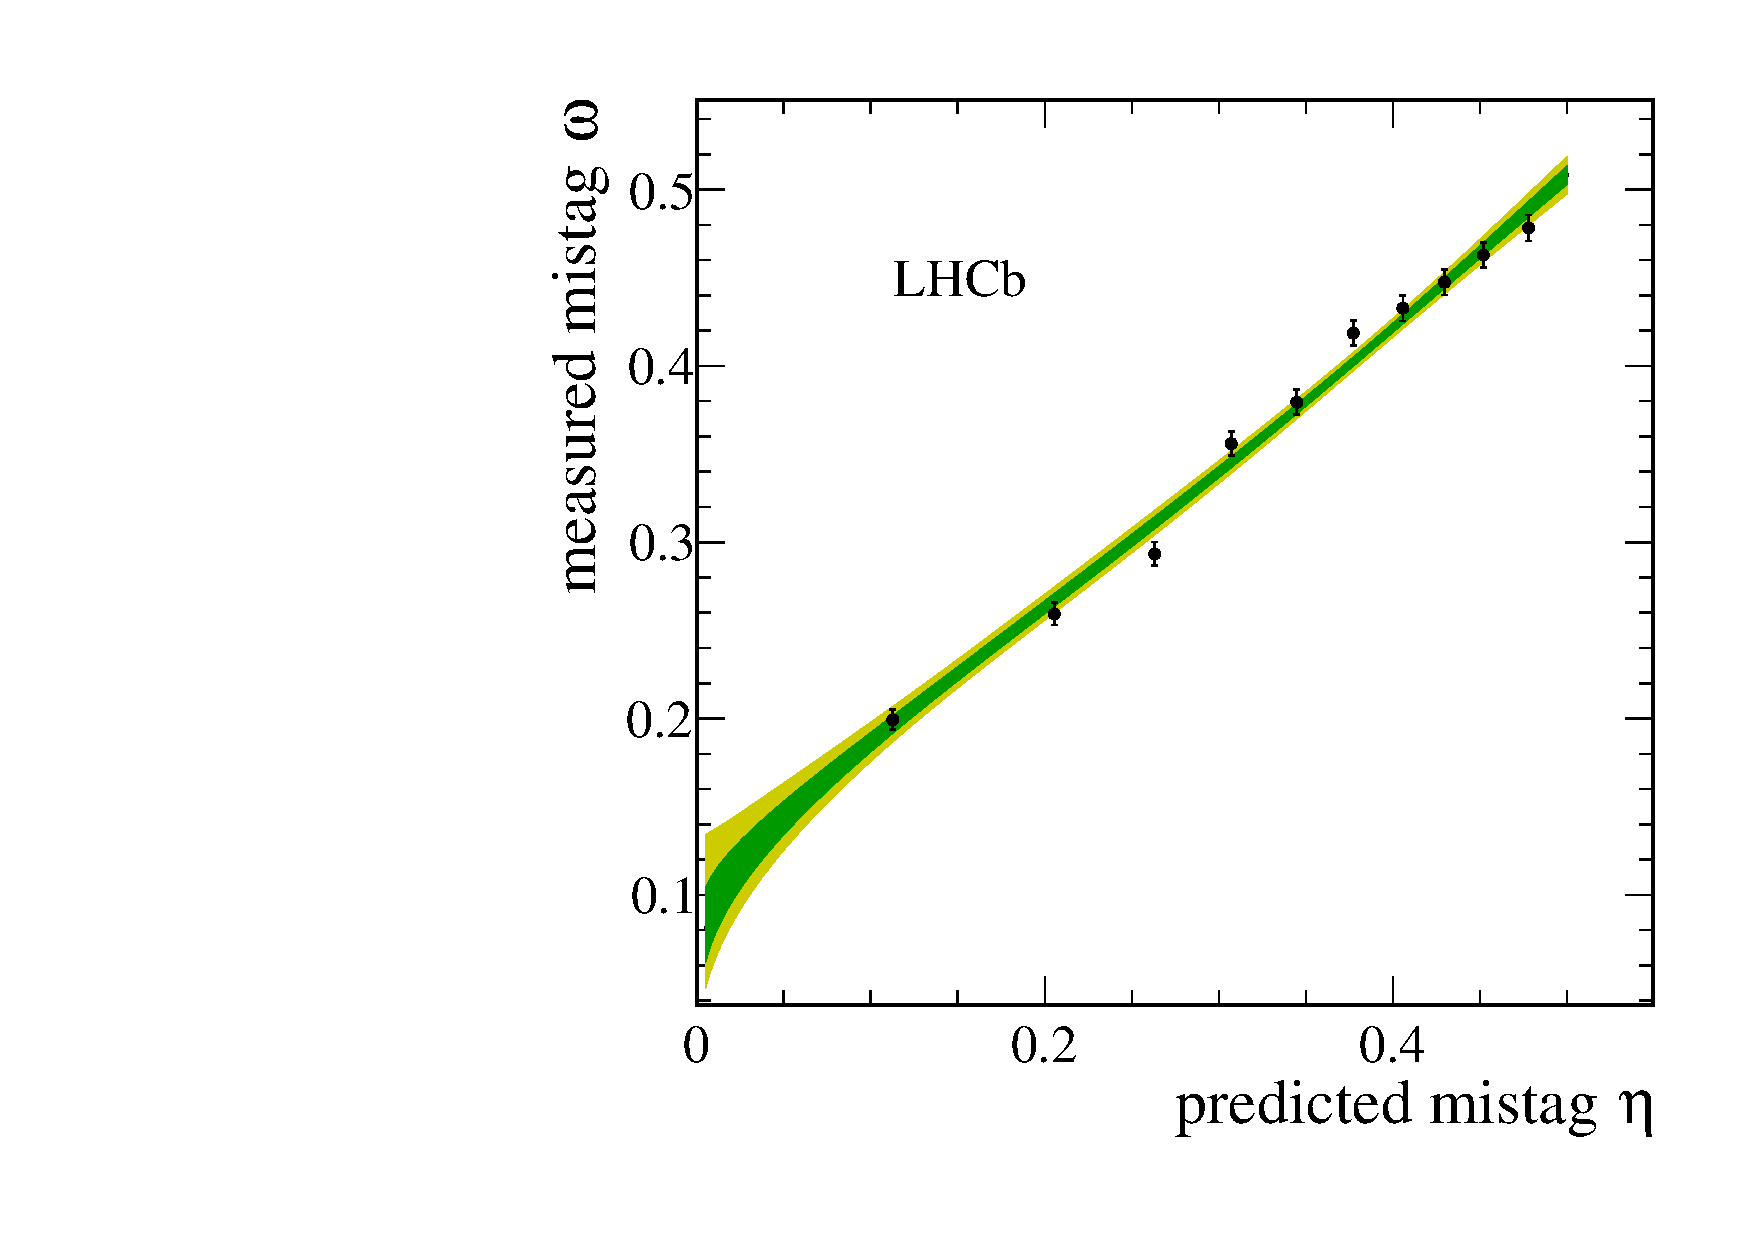
\includegraphics[width=0.26\textwidth]{04FlavourTagging/figs/OSelectronOpt/run2b2oc_tunings/OS_Combination_Calibration.pdf} \\
  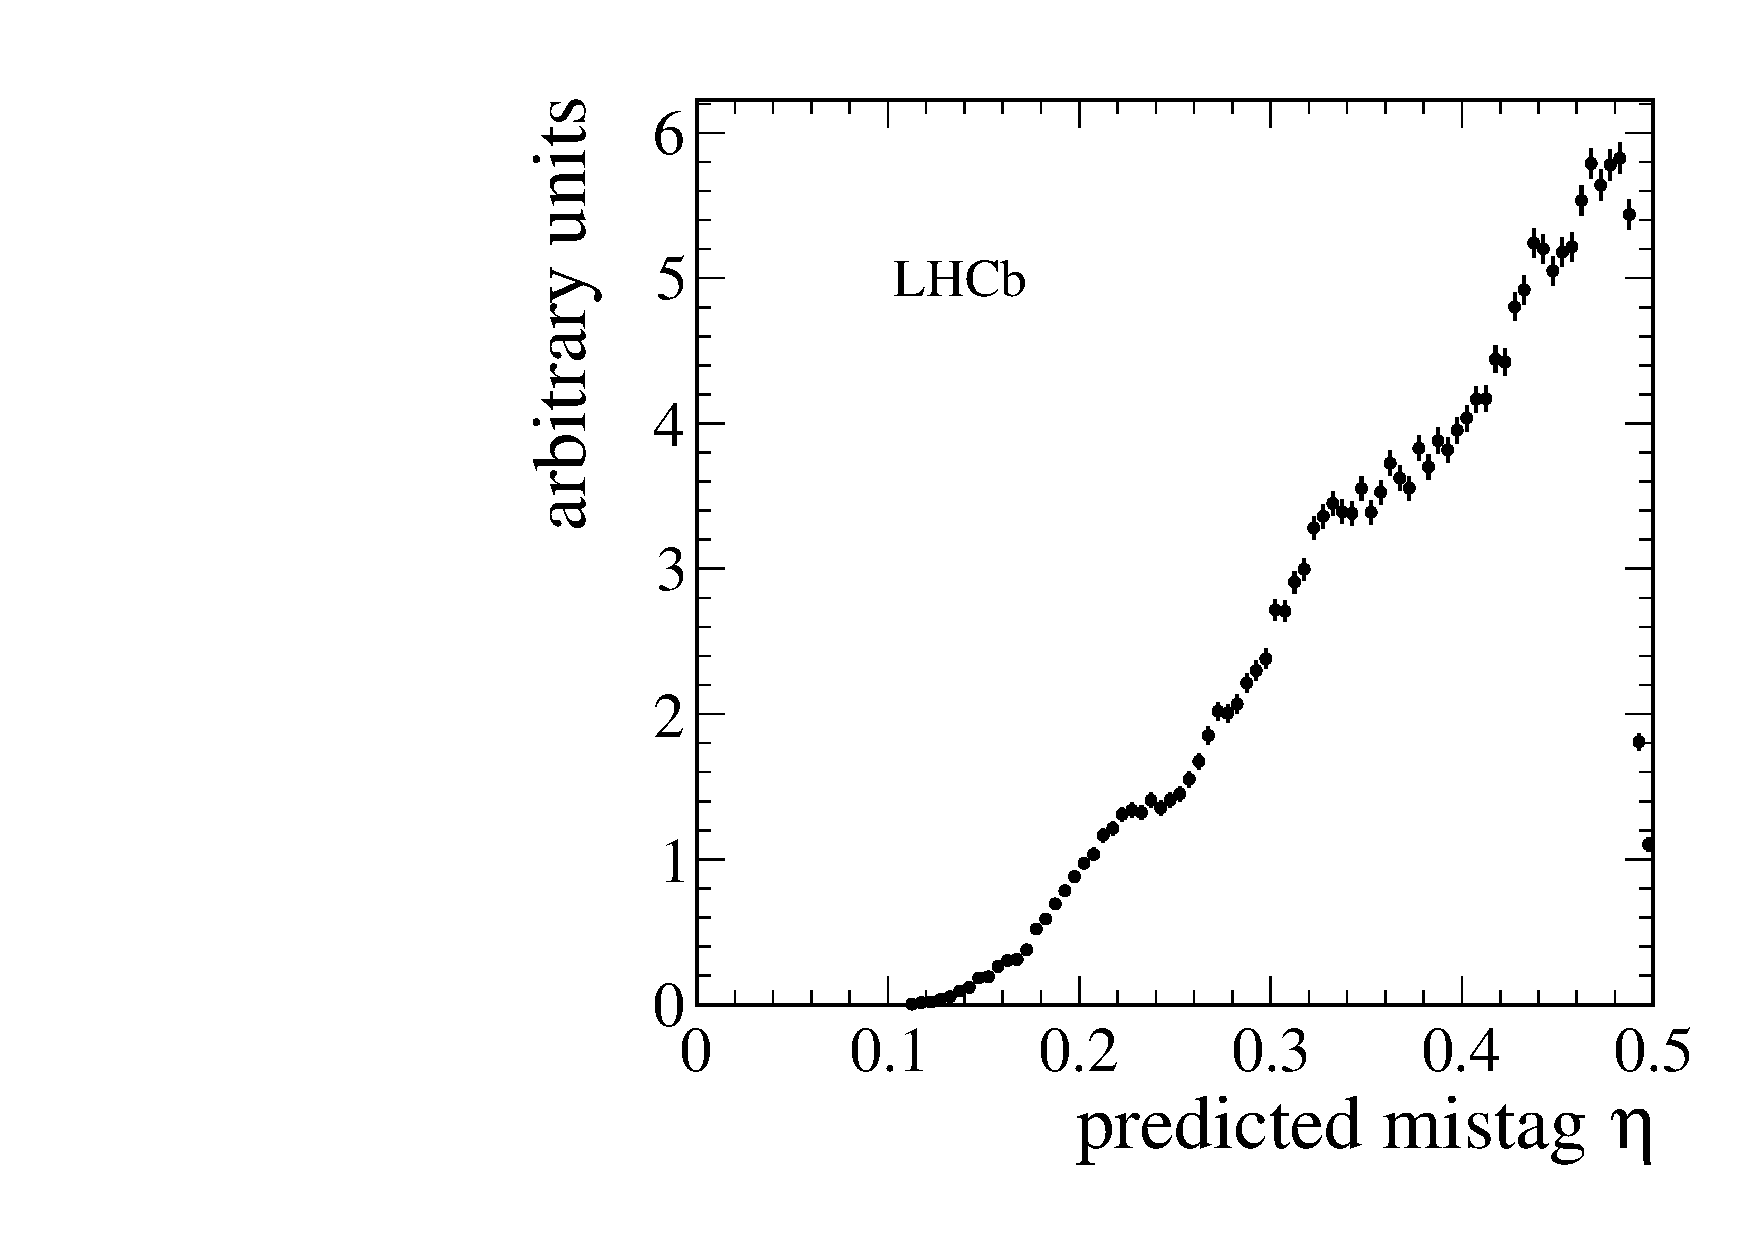
\includegraphics[width=0.26\textwidth]{04FlavourTagging/figs/OSelectronOpt/run1_tunings/OS_Combination_EtaDist.pdf}
  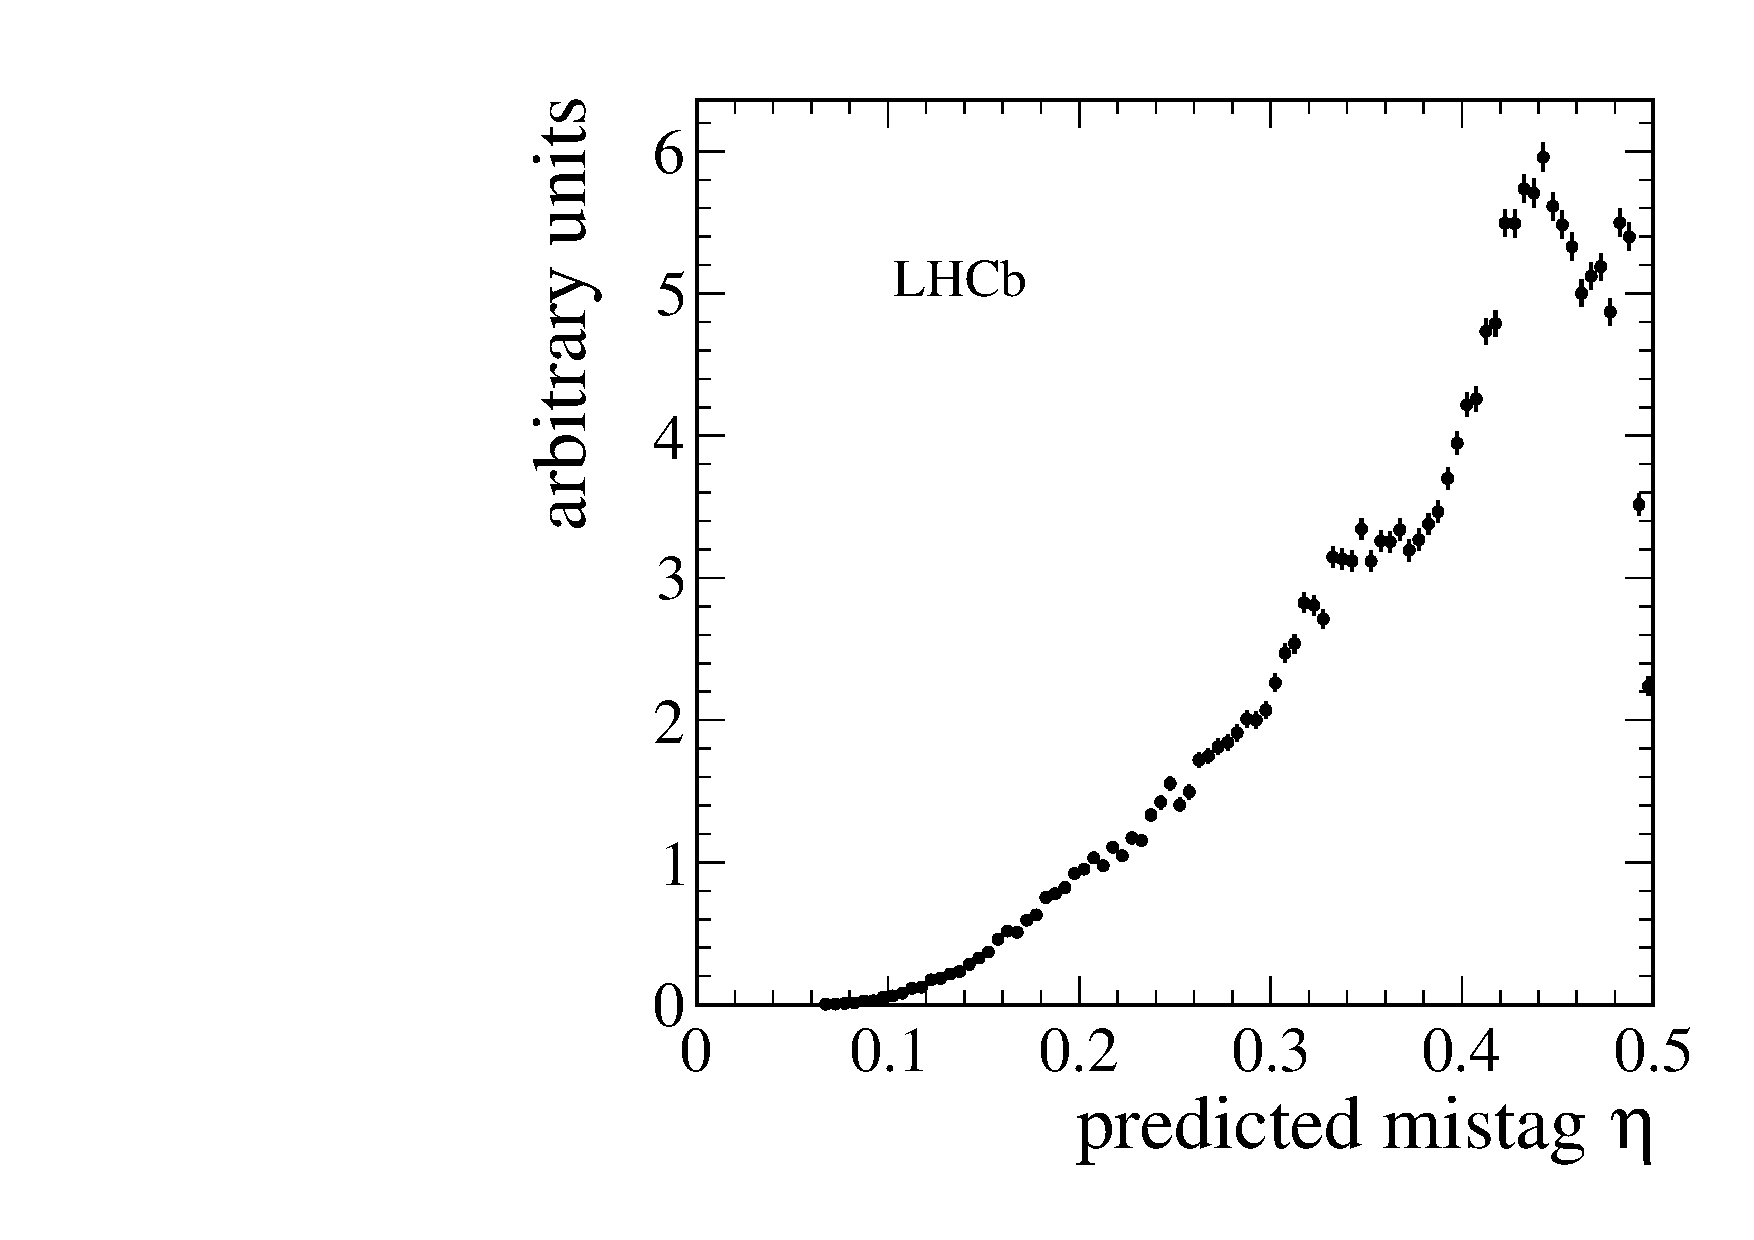
\includegraphics[width=0.26\textwidth]{04FlavourTagging/figs/OSelectronOpt/run2b2cc_tunings/OS_Combination_EtaDist.pdf}
  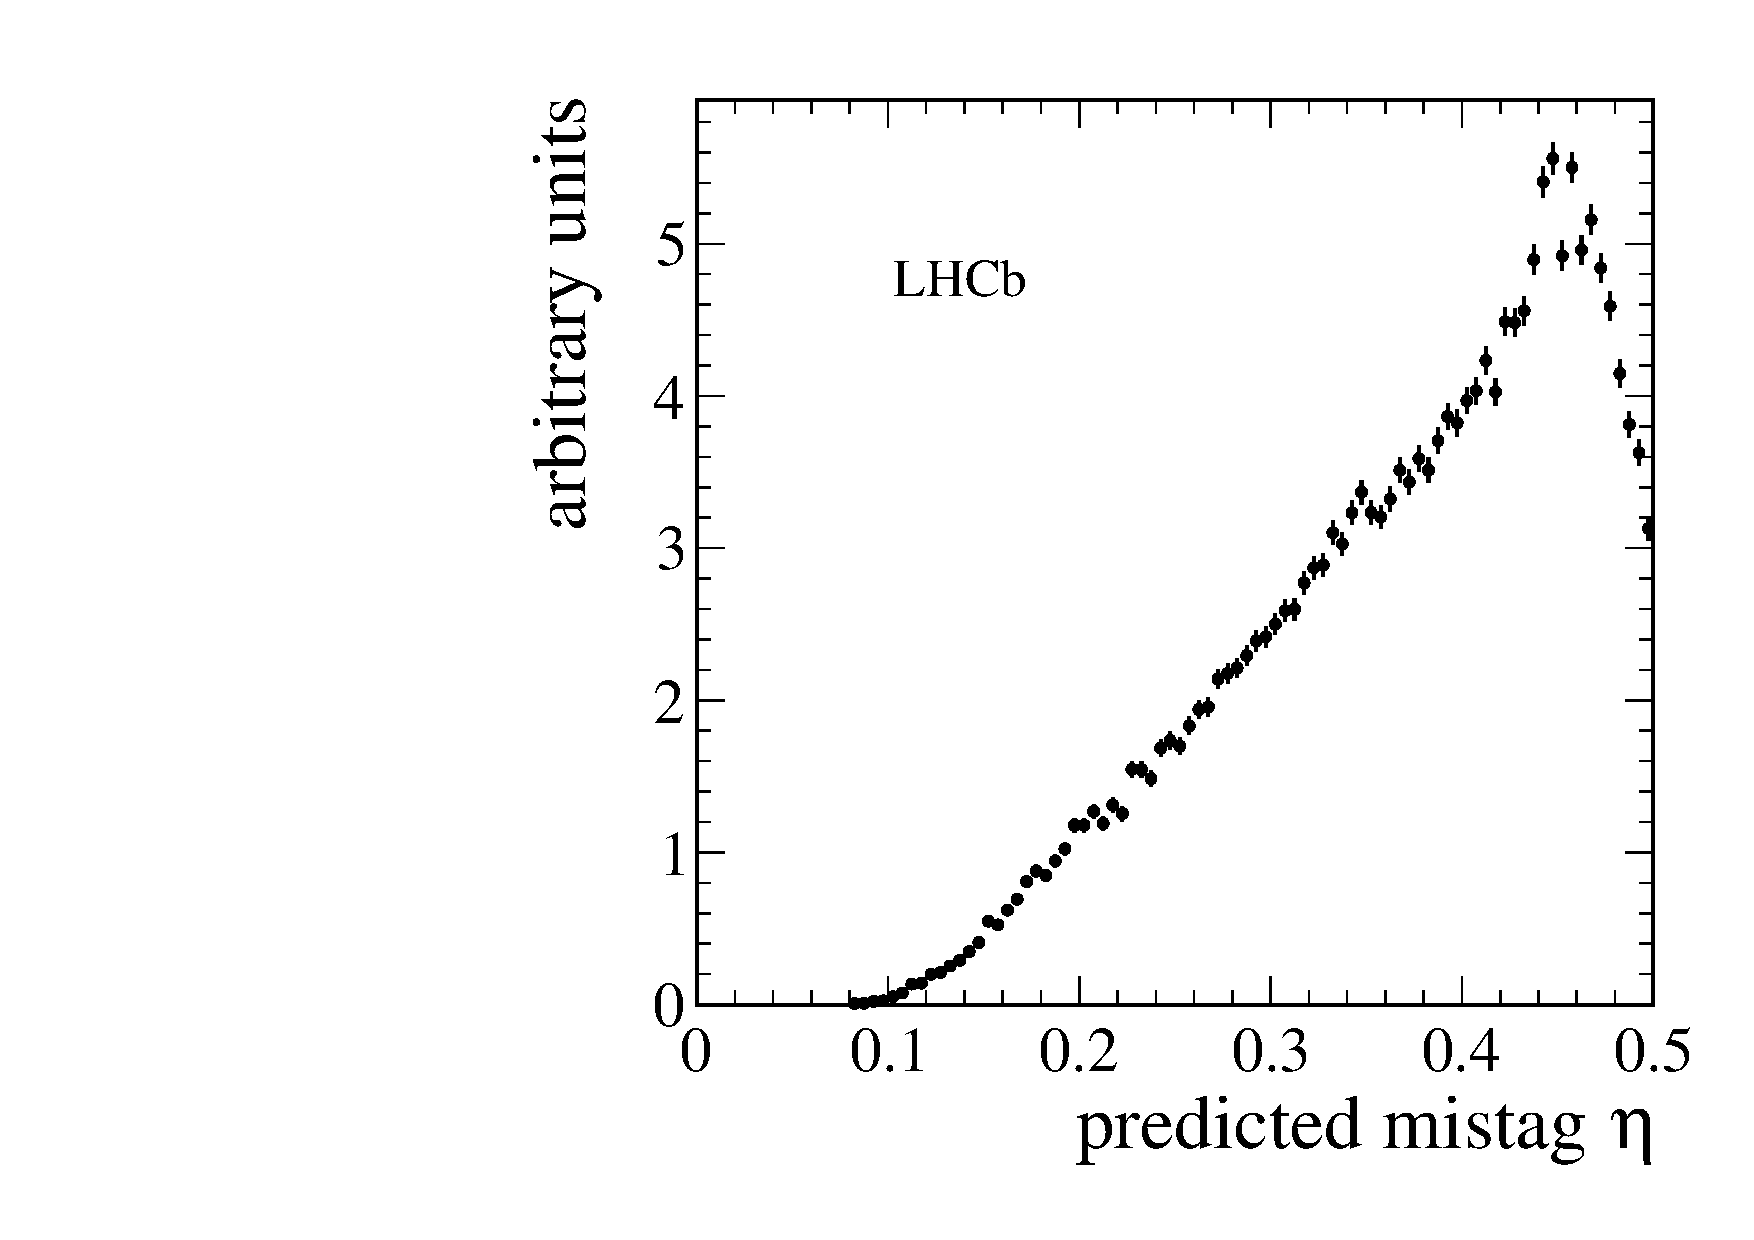
\includegraphics[width=0.26\textwidth]{04FlavourTagging/figs/OSelectronOpt/run2b2oc_tunings/OS_Combination_EtaDist.pdf}
  \vspace{-2mm}
  \caption{Mistag calibration results on \emph{sWeighted} Run 2 $B^0\to D^-\pi^+$ data for the combination of the OS taggers. The results obtained with the Run 1 old (left), Run 2 B2CC (center), and Run 2 B2OC (right) tunings of \OSe, \OSmu, and \OSK~are shown. The \emph{sWeighted} data sample is shown as black points. The green (yellow) band indicates the 68\% (95\%) C.L. interval for the fitted calibration functions. Bottom: distributions of the uncalibrated mistag $\eta$.}
  \label{fig:OSePerfCalib4}
\end{figure}

The performance is reported in Tables~\ref{tab:Bd2DpiperformanceRun1}~and~\ref{tab:Bd2DpiperformanceRun2}.
The Run 1 new tuning allows to gain a relative $~9\%$ in tagging power for the \OSe~tagger on Run 1 data; the corresponding, relative gain of the OS combination is $~3\%$.
The tagging power of \OSvtx~and \OSc, which were trained on Run 1 data, increases on Run 2 data compared to Run 1; 
for this reason, no specific optimisation for the Run 2 conditions is performed.
The tagging power of \OSe, \OSmu, and \OSK~with the Run 1 tunings is lower on Run 2 data compared to Run 1. 
However, compared to the Run 1 tunings, the Run 2 tunings show a relative improvement in tagging power of about $\sim 160\%$ for \OSe, and $\sim 6\%$ for \OSmu~and \OSK~on Run 2 data. This allows to recover similar performances as the ones obtained on Run 1 data with the Run 1 tunings, both for the individual taggers and their combination.
Moreover, the Run 2 B2CC and B2OC tunings show consistent tagging powers on Run 2 data, meaning that the optimisation is robust against the different kinematics of the adopted decays.

\begin{table}
\centering
\caption{Performance (tagging efficiency, average mistag and tagging power in $\%$) of the OS taggers on \emph{sWeighted} Run 1 $B^0\to D^-\pi^+$ data. The numbers for \OSe~and the OS combination are shown separately for the Run 1 old and Run 1 new tunings. The first uncertainty is statistical and the second comes from the calibration.}
\label{tab:Bd2DpiperformanceRun1}
%\resizebox{\textwidth}{!}{
\begin{tabular*}{\textwidth}{rlllll}
\toprule
\multicolumn{1}{c}{Tagger} & \multicolumn{1}{c}{$\etag$} & \multicolumn{1}{c}{$\avg{\mistag}$} & \multicolumn{1}{c}{$\effeff$} \\
\midrule
\OSvtx& $22.026\pm0.100$& $37.295\pm0.030\pm0.376$& $1.422\pm0.009\pm0.084$\\
\OSc& $4.632\pm0.050$& $34.026\pm0.049\pm0.824$& $0.473\pm0.006\pm0.049$\\
\hline
\OSe~Run 1 old& $3.028\pm0.041$& $30.570\pm0.113\pm0.963$& $0.457\pm0.008\pm0.045$\\
\OSe~Run 1 new& $4.337\pm0.049$& $33.089\pm0.085\pm0.777$& $0.496\pm0.007\pm0.046$\\
\hline
\OSmu~Run 1& $8.539\pm0.067$& $28.756\pm0.071\pm0.582$& $1.541\pm0.016\pm0.085$\\
\hline
\OSK~Run 1& $18.800\pm0.094$& $36.724\pm0.031\pm0.417$& $1.325\pm0.009\pm0.083$\\
\hline
\begin{tabular}{c} OS combination \\ Run 1 old \end{tabular}& $39.004\pm0.117$& $34.679\pm0.035\pm0.273$& $3.662\pm0.020\pm0.131$\\
\begin{tabular}{c} OS combination \\ Run 1 new \end{tabular}& $39.733\pm0.118$& $34.576\pm0.035\pm0.270$& $3.781\pm0.021\pm0.133$\\
\bottomrule
\end{tabular*}
%}
\end{table}

\begin{table}
\centering
\caption{Performance (tagging efficiency, average mistag and tagging power in $\%$) of the OS taggers on \emph{sWeighted} Run 2 $B^0\to D^-\pi^+$ data. The numbers for \OSe, \OSmu, \OSK, and the OS combination are shown separately for the Run 1, Run 2 B2CC, and Run 2 B2OC tunings. The first uncertainty is statistical and the second comes from the calibration.}
\label{tab:Bd2DpiperformanceRun2}
%\resizebox{\textwidth}{!}{
\begin{tabular*}{\textwidth}{rlllll}
\toprule
\multicolumn{1}{c}{Tagger} & \multicolumn{1}{c}{$\etag$} & \multicolumn{1}{c}{$\avg{\mistag}$} & \multicolumn{1}{c}{$\effeff$} \\
\midrule
\OSvtx& $20.834\pm0.075$& $36.139\pm0.029\pm0.301$& $1.601\pm0.009\pm0.070$\\ 
\OSc& $5.025\pm0.040$& $33.875\pm0.041\pm0.624$& $0.523\pm0.005\pm0.040$\\
\hline
\OSe~Run 1 old& $1.868\pm0.025$& $34.300\pm0.096\pm0.941$& $0.184\pm0.003\pm0.022$\\
\OSe~Run 2 B2CC& $4.451\pm0.038$& $33.352\pm0.081\pm0.608$& $0.493\pm0.006\pm0.036$\\
\OSe~Run 2 B2OC& $3.333\pm0.033$& $30.917\pm0.075\pm0.702$& $0.486\pm0.006\pm0.036$\\
\hline
\OSmu~Run 1& $8.343\pm0.051$& $30.357\pm0.042\pm0.466$& $1.288\pm0.010\pm0.061$\\
\OSmu~Run 2 B2CC& $9.151\pm0.053$& $30.837\pm0.041\pm0.432$& $1.344\pm0.010\pm0.061$\\
\OSmu~Run 2 B2OC& $8.040\pm0.050$& $29.174\pm0.043\pm0.463$& $1.395\pm0.010\pm0.062$\\
\hline
\OSK~Run 1& $15.737\pm0.067$& $35.902\pm0.030\pm0.357$& $1.251\pm0.008\pm0.063$\\
\OSK~Run 2 B2CC& $19.516\pm0.073$& $36.889\pm0.026\pm0.310$& $1.342\pm0.007\pm0.064$\\
\OSK~Run 2 B2OC& $15.793\pm0.067$& $35.565\pm0.030\pm0.348$& $1.316\pm0.008\pm0.063$\\
\hline
\begin{tabular}{c} OS combination \\ Run 1 old \end{tabular}& $36.239\pm0.088$& $35.285\pm0.024\pm0.227$& $3.139\pm0.013\pm0.097$\\
\begin{tabular}{c} OS combination \\ Run 2 B2CC \end{tabular}& $40.154\pm0.090$& $35.123\pm0.025\pm0.210$& $3.555\pm0.014\pm0.100$\\
\begin{tabular}{c} OS combination \\ Run 2 B2OC \end{tabular}& $36.555\pm0.089$& $34.225\pm0.026\pm0.220$& $3.638\pm0.015\pm0.102$\\
\bottomrule
\end{tabular*}
%}
\end{table}
